 \documentclass[oneside,11pt]{article}


\usepackage{soul}
\usepackage{natbib}
\usepackage{hyperref}
\usepackage{graphicx}             
\graphicspath{{./Figuras/}}

\usepackage{makecell}
\usepackage[margin=1.0in]{geometry}
\usepackage{float}                
\usepackage{amsmath}
\usepackage{amscd}
\usepackage{amsfonts}
\usepackage{amssymb}
\usepackage{bbm}
\usepackage{booktabs}
\usepackage{nameref}
\usepackage{multirow}
\usepackage[nokeyprefix]{refstyle}
\usepackage{rotating}
\usepackage{threeparttable}
\usepackage{lscape}
\usepackage{enumerate}
\usepackage{afterpage}
\usepackage{caption}
\usepackage{subcaption}
\usepackage{epstopdf}
\epstopdfDeclareGraphicsRule{.tiff}{png}{.png}{convert #1 \OutputFile}
\AppendGraphicsExtensions{.tiff}

\epstopdfDeclareGraphicsRule{.tif}{png}{.png}{convert #1 \OutputFile}
\AppendGraphicsExtensions{.tif}

\usepackage{tikz}
\usetikzlibrary{shapes.geometric, arrows}
\usetikzlibrary{calc}
\usetikzlibrary{matrix}

\tikzset{ 
    table/.style={
        matrix of nodes,
        row sep=-\pgflinewidth,
        column sep=-\pgflinewidth,
        nodes={
            rectangle,
            draw=black,
            align=center
        },
        minimum height=1.5em,
        text depth=0.5ex,
        text height=2ex,
        nodes in empty cells,
%%
        every even row/.style={
            nodes={fill=gray!20}
        },
        column 1/.style={
            nodes={text width=2em,font=\bfseries}
        },
        row 1/.style={
            nodes={
                fill=black,
                text=white,
                font=\bfseries
            }
        }
    }
}


\usepackage{colortbl}

\newtheorem{theorem}{Theorem}
\newtheorem{claim}[theorem]{Claim}



%%% HELPER CODE FOR DEALING WITH EXTERNAL REFERENCES
\usepackage{xr}
\makeatletter
\newcommand*{\addFileDependency}[1]{
  \typeout{(#1)}
  \@addtofilelist{#1}
  \IfFileExists{#1}{}{\typeout{No file #1.}}
}
\makeatother


\newcommand*{\myexternaldocument}[1]{
    \externaldocument{#1}
    \addFileDependency{#1.tex}
    \addFileDependency{#1.aux}
}

%\myexternaldocument{OA}

%%%%%%%%%%%%%%%%%%%%%%%%%%%%%%%% DOCUMENT
\begin{document}


\title{The limits of self-commitment and private paternalism \thanks{We want to thank Mauricio Romero and Anett John for advice and encouragement. Ricardo Olivares, Gerardo Melendez, and Alonso de Gortari provided excellent research assistance and Erick Molina helped with formatting. Jose Maria Barrero, Andrei Gomberg, Emilio Gutierrez, David Laibson, Aprajit Mahajan, Matt Rabin, Charlie Sprenger, and seminar participants at ITAM provided valuable feedback.}}
\author{Craig McIntosh \and Isaac Meza \and Joyce Sadka \and Enrique Seira \and Francis J.\ DiTraglia   \thanks{Seira: ITAM/MSU, \url{enrique.seira@gmail.com} (corresponding author); McIntosh:  University of California San Diego, \url{ctmcintosh@ucsd.edu}; Meza: Harvard University, \url{isaacmezalopez@g.harvard.edu}; Sadka: ITAM, \url{jsadka@itam.mx}; DiTraglia: Oxford, \url{francis.ditraglia@economics.ox.ac.uk}} }
\date{This draft:  \today \\[2 cm]}

%\vspace{.5in}


\maketitle
\thispagestyle{empty}
\begin{abstract}

%Many firms provide commitment devices that restrict individuals' choice, but shroud this. Shrouding suggests low demand for commitment. We show that private paternalism is beneficial in the pawnbroker context we study. 

In the context of pawnbroker lending, we show that forcing people into commitment contracts with financial penalties for not paying on time \textit{decreases} their (fee-including) financial cost by 9.4\%, increases the likelihood of recovering their pawn by 26\%, and increases the likelihood of repeat business by almost 100\%. Using machine learning methods for estimating heterogeneous treatment effects, we find that more than {70}\% clients would reduce their financing cost with the commitment contract, however only 10\% choose it. Those that \textit{don't} choose it are predicted to be the ones who would benefit more. Relying on personal promises instead of fees as commitment triples take-up but has no effects on outcomes.

%and one of the most understudied. In our context more than on half of borrowers default and lose their pawn and whatever they have paid towards recovering it. Compared to the status quo pay-at-anytime 3-month contracts, forcing borrowers to pay monthly and charge a penalty if they didn't --i.e. a commitment contract-- increased recovery of pawn by about 30\% and financial costs by 10\%. However when offered a choice between the two contracts only 10\% took the monthly payment one. A pecuniary commitment seems necessary. In an alternative arm, we made them promise to pay but removed the pecuniary penalty. This increased take up to 31\%, but had zero effect on financing cost or default. The forcing contract may be better than choice for naive present biased consumers.

\end{abstract}

\vspace{.3in}

\textbf{Keywords: } Private paternalism, choice, present bias, naivete, overconfidence, commitment, heterogeneous treatment effects.

\textbf{JEL codes:} G41, C93, O16, G21

\newpage

\pagenumbering{arabic}
\etocdepthtag.toc{mtchapter}
\etocsettagdepth{mtchapter}{subsection}
\etocsettagdepth{mtappendix}{none}


%NO MORAL HAZARD IN THE CONTRACT SINCE FULLY COLLATERALIZED
%DOUBLE FAILURE: DEMAND LOW, AND DOES NOT WORK BY PEOPLE WHO TAKE IT.
%PENALIZES THEM EVEN MORE ON SOMETHING THEY WERE ALREADY PENALIZED 
%PROPENSITY TO CHOSE.
%PULLING PUNISHMENT FORWARD --CHARGING RIGHT WHEN I MESS UP.
%MAYBE ONLY IMPATIENT AND NAIVE END IN PAWNSHOPS
%1) SELECT A RANDOM SAMPLE OF NEIGHBORHOODS, EXTERNAL VALIDITY, THE ONES THEY GO ARE NAIF AND
%HYPERBOLIC
%2) ASK TO CHOSE AMONG ALL CONTRACTS
%3) CLASSIFY SOPHISTICATION AT BASELINE
%4) HOW TO GET AT SHOCKS.  --BUT DOES NOT SQUARE WITH WHY CHARGING THEM FEES WORKE.
%do shocks vary across strata, predict shocks.
%DEEP BEHAVIORAL PAPER -- CAN WE REALLY PREDICT?



\section{Introduction}

Restrictions of choice are often surreptitiously imposed on consumers. Firms limit their worker's freedom by requiring time-consuming progress reports,  schools impose deadlines and pop quizzes, and loan contracts often require monthly repayment. As pointed out by \cite{Laibson2018}, although these choice-restricting mechanisms may be beneficial to firms and clients, they are often disliked by the latter, and therefore ‘shrouded’ by firms, i.e. not advertised but nonetheless embedded in products. \cite{Laibson2018} coins the term ``private paternalism'' for cases when restrictions on the freedom of choice is implemented by a firm in a way that advances a client's interests. 

Although the examples above are plausible, substantiating a case for private paternalism is not easy. It involves comparing the causal effect of forcing a certain product characteristic versus the effect of letting people choose on that characteristic. This is not an easy task because a given person wither has or does not have choice, and because choice induces selection, potentially biasing causal estimates. A large behavioral literature has illustrated that allocating borrowers to a commitment-savings product increase savings \citep{thaler2004save, prina2015banking, brune2016facilitating, callen2019headwaters, Pascaline, Ashraf}, but this literature does not show that commitment would not be chosen by those that would benefit from it, that is, that the Treatment Effect on the Untreated (TuT) is positive. In fact, selection on gains has such wide acceptance that economists often impose it in their models \hl{CITES}. In microfinance, a context close to ours, \citep{Murdoch} claim that there exists positive selection, citing a positive correlation between displaying present biased preferences in surveys and selecting into microfinance as evidence of borrowers' actually demanding the discipline imposed by frequent payments. However, they are unable to show that borrowers indeed benefit or that they indeed positively select based on treatment effects.

%Many people have a difficult time accumulating and retaining capital unless they are provided a structure within which to do so.  The behavioral lens on intertemporal financial services has provided critical insights on this problem, suggesting that saving from cash-in-hand is challenging \citep{Ashraf, Pascaline}, that credit may be preferred to savings as a way of accumulating capital simply because credit repayment contracts provide more structure \cite{Murdoch}, and even that the absence of structured financial contracts may be a key barrier preventing the poor from climbing out of poverty \citep{bertrand2004behavioral, collins2009portfolios}.  A large behavioral literature has illustrated that the addition of commitment-style product features improves the ability to accumulate savings \citep{thaler2004save, prina2015banking, brune2016facilitating, callen2019headwaters} and to retire debt \citep{Bertrand, heidhues2010exploiting}.  As a consequence, credit markets featuring limited-liability loans such as small-business financing or microfinance typically take a highly structured approach to credit contracts with frequent repayments and reminders as a way of inducing repayment.  As pointed out by \cite{Laibson2018}, because many of these forms of commitment may be desirable to principals but not demanded by agents (or by the right agents), these mechanisms are often ‘shrouded’, meaning that commitment is embedded in products in ways that are not advertised to clients as such.

This paper studies the benefits of restricting choice in the context of pawnbroker lending. Pawn loans are one of the oldest, most understudied, and most prevalent forms of borrowing \citep{carter2012pawnshops}. There are more than 11,000 pawn shops across the US, with 30 million clients and \$14 billion yearly revenues (in China it is a 43 billion dollar industry).\footnote{\url{https://tinyurl.com/ybm56dpe}, \url{https://tinyurl.com/y9zdcgws}, \url{https://tinyurl.com/y59ptdam}.} Our partner pawn lender (henceforth Lender $P$) alone served more than 1 million clients in the last 3 years with more than 4 million contracts.\footnote{For comparison there were 2.3 million micro-finance clients in Mexico in 2009 (\cite{Pedroza:2010}).} Pawnshop lending presents an inverted lending case: since these loans are over-capitalized, the principal in the lending contract stands to gain the most when agents default. 

Our collaborating pawn lender (henceforth Lender P) gave 70\% of the value of the pawn in credit, and charged a monthly interest rate of 7\% for loans of a three-month duration, with a flexible no-reminders contract typical of the industry that can be paid back anytime before the loan comes due at no penalty. This combination of features, and the fact that the gold pawn is highly liquid, means that the lender makes 90\% more profit over three months for a borrower who defaults than one who repays (30\% of collateral value recovered under default, 15.8\% of collateral value paid in interest if loan fully repaid). While an older literature considers the exploitative potential in over-collateralization and underpricing of collateral \citep{basu1984implicit}, the implication of such contracts has not been analyzed in the behavioral literature.  %When the lender desires default, the repayment-inducing features of commitment-style repayment contracts become undesirable and there may be incentives for the principal to create contracts with no structure, no reminders, and simple balloon payments. 
To repurpose the language of \cite{Laibson2018}, we suggest that pawn contracts effectively shroud their \textit{lack} of commitment features to induce default in a manner not obvious to borrowers. Given that pawnshops, moneylenders, and paycheck lending institutions are likely to face client pools disproportionately made up of impatient and time-inconsistent individuals, the design of such contracts may have serious consequences for the financial lives of the poor.

%clients lose their pawn, and among those that recover it almost all of them pay in the last days, just before the loan elapses.\footnote{In the US default is also high at 15\% (\url{https://tinyurl.com/yc2x5bjf}).}

%In this paper we examine pawn contracts, an understudied form of credit despite their relative ubiquity \citep{carter2012pawnshops}, and a major vehicle through which poor households may dis-accumulate savings.  There are more than 11,000 pawn shops across the US, with 30 million clients and \$14 billion yearly revenues.  In China it is a 43 billion dollar industry.\footnote{\url{https://tinyurl.com/ybm56dpe}, \url{https://tinyurl.com/y9zdcgws}, \url{https://tinyurl.com/y59ptdam}.} Our partner, a Mexican pawn lender (henceforth Lender $P$) alone served more than 1 million clients in the last 3 years with more than 4 million contracts.  

Against this backdrop, we implement a multi-arm randomized control trial covering close to 10,000 pawnshop clients in 6 branches of Lender $P$ in Mexico City, using a design built to test the demand for and impact of payment structure in pawn repayment contracts. Our control arm illustrates the costs of the status quo contract; fully 57\% of borrowers default and so lose their pawn.\footnote{These high default rates are not uncommon, in the US default is also high at 15\% (\url{https://tinyurl.com/yc2x5bjf}).} We then implement a `commitment choice’ arm, in which borrowers are able at the time of taking a loan to opt in to a structured repayment contract, in which they are asked to make three monthly payments rather than one balloon payment at the end, with each monthly payment including the accrued interest at that time, and borrowers levied a nominal fee of 2\% of that month's payment in case of delinquency as a reminder/reinforcement of the importance of these interim payments. In addition, we include a `forced commitment’ arm, in which all borrowers are required to repay using the monthly payment structure. 

The combination of voluntary and forced commitment within the RCT allows us to address several key questions.  First, does using more structured repayment contracts help pawnshop borrowers to save on financing cost. Second, do borrowers recognize this benefit, demanding commitment in sufficient numbers?  Finally, and most uniquely, because we incorporate the forced commitment arm, we are able to ask whether the \textit{right} borrowers voluntarily demand commitment, gaining point identification for the Treatment on the Treated (ToT) and the Treatment on the Untreated (TuT), using the control, choice, and forced arms. 
	
Our results suggest that the structure of the commitment is strongly effective in preventing default, with the average individual in the forced arm paying financing costs inclusive of fees that are \hl{20\%} lower than the control, while default decreases by 6.5 percentage points (15\% of the mean). In terms of Annual Percentage Rates, the financial cost of borrowing is reduced by 34 percentage points. That is, imposing commitment structure it is possible to save borrowers money by charging them fees! These results are robust qualitatively to including transport costs of going to the branch plus losing a day's wage for each visit, using the subjective instead of the gold value of the pawn, and imputing some adjustment for liquidity lost by requiring monthly payments. 

The monthly payment contract seems to be achieving these cost savings by speeding up payments and by generating an early bifurcation of borrowers into those that will recover the pawn and those that will not, saving the later payments towards recovery. In the treatment group, the first payment occurs 13 days earlier, the fraction recovering on the first visit by is 7.9 percentage point higher. Commitment contract decreases fraction of borrowers making a payment and not recovering by 7 percentage points. \hl{Treatment effects are concentrated in the intensive margin as treatment does not affect the fraction of clients who pay a positive amount towards pawn recovery. That is, the commitment contract induces people who would otherwise pay something towards recovery, to pay more and faster, making them more likely to recover their pawn at a lower financial cost.} 

In spite of a large average treatment effect documenting financial cost savings, given the opportunity in the choice arm, only 11\% of borrowers actually choose commitment. If the effect of commitment were homogeneous, this would be enough to conclude that the 89\%
who did not choose it would have been financially better off if they had. However, we test and reject the null hypothesis of homogeneous treatment effects using the method of \cite{chernozhukov2018generic}. Can the borrowers who did not choose commitment be those who simply don’t need it? We address this question by sequentially imposing more structure in the problem. 

\hl{We start by bounding the distribution of treatment effects $Y_{1i}-Y_{0i}$ using the two marginal distribution } in the treatment and control arms as in \cite{fan2010sharp}. We find that at least 30\% of individual borrowers benefit from commitment, implying many borrowers did not demand even though the treatment effect would be positive for them. Then, we impose the mild exclusion restriction that the effect of the contract does not depend on how they got it, that is: choosing a contract has the same treatment effect as being assigned to the contract.\footnote{This is a frequently used assumption even if often implicit. For instance, a significant literature uses schooling compulsory laws to estimate the return of one more year of school, and then often interprets that schooling, in general, has this return.} We show that in this case our 3-armed experiment point identifies the TuT. We then estimate that the financial cost savings of the TuT is large, at \$356 pesos, equivalent to 24 percentage point savings in APR. That is, on average borrowers that did \textit{not} choose the frequent payment contract would have benefited from having that contract.\footnote{We estimate a positive ToT that is larger than the TuT, but it is imprecise\footnote{This results from the smaller sample size, given that few chose the monthly payment contract.}, and the hypothesis of ToT=TuT is rejeted only with 13 percent confidence for the APR and 12 percent confidence for default.}  We also estimate that those that would not choose if given the opportunity would have lower status-quo outcomes (i.e. the average selection bias is negative). Finally, assuming the exclusion restriction for subsets of observable characteristics splits generated by a causal forest allows us to establish that \hl{70\%} of would-be non-choosers would save on financial cost by being assigned to frequent payments. That is, the benefits of imposing a monthly payment are distributed broadly. \hl{TuT benefits are particularly large for XXX CHARACTERISTICS, and ToT benefits for those with XXX.} 

\textcolor{brown}{In a final step, we use the Causal Random Forest algorithm of \cite{atheygrf} to estimate individual-level treatment effects for the forced versus control arm, and show the benefits of forcing to be significantly negatively correlated with the propensity to choose commitment estimated from the choice arm.  93\% of those who did not opt for the commitment contract would have been better off with it, while only 1\% of those who chose commitment would have been better off without it.} \textcolor{blue}{Targeting frequent payment products to those that benefit the most is a policy that should be explored. In this context we calculate \hl{XXX}.}

%however those most economically vulnerable, and those most overconfident about their probability of repayment, experience larger gains.

%\footnote{As in \cite{Rabin2018} we contrast subjects' \textit{own predictions} of their behavior with their actual behavior, but we do it in a natural setting.}  

%Borrowers assigned to the forced commitment contract are 5 percentage points (100\% of the mean) more likely than the control group to ask for another loan in the future, suggesting that they liked the commitment contract after experiencing it.  However, when offered the choice of commitment, very few borrowers elect to commit voluntarily.  Only 10\% of the choice arm takes up the contract, and none of the core study outcomes are significantly improved by the ability to choose commitment.  

%This is not the first paper to find low demand for commitment, however it is the first we know of that can compare choice versus forcing with a money-metric outcome such as loan repayment. 

%Most importantly, our multi-arm design allows us to show that the \textit{wrong} people choose commitment when offered it.   We illustrate this point in three distinct ways.  First, we use a Random Forest algorithm \citep{atheygrf} to estimate individual-level treatment effects for the forced versus control arm, and show the benefits of forcing to be significantly negatively correlated with the propensity to choose commitment estimated from the choice arm.  93\% of those who did not opt for the commitment contract would have been better off with it, while only 1\% of those who chose commitment would have been better off without it.  Second, a Boosted Classification Algorithm arrives at a similar answer, showing that the borrowers naturally cluster into two groups, one of which is likely to choose commitment and does not benefit from it, and the other the reverse.  Finally, estimating LATEs on compliers and non-compliers alike we show that the estimated treatment effect on non-compliers is larger than the treatment effect on compliers.  That is, those choosing commitment benefit less from commitment than those not choosing it.  Hence our results show clearly that a paternalistic policy forcing borrowers into a more rigid and structured repayment regimen is uniquely beneficial to them.  While this perverse relationship between choice and benefits from commitment echo closely the findings of \cite{Sprenger} we are the first to be able to examine this relationship using a high-stakes, money-metric outcome in a natural field environment.


What explains the persistence of a contract so contrary to borrowers’ interests?  First, we show substantial levels of over-optimism among borrowers.  Those most likely to benefit from the commitment contract and \textit{not} choose it are the individuals who most systematically over-estimate their own probability of repayment at the time of taking the loan.\footnote{More generally \hl{demand for commitment is higher among those with XXX characteristics.}}  Second, the existence of commitment-style repayment contracts in pawnshop lending is novel in Mexico. The dramatic improvements in borrower income arising from the commitment contract come directly from the pockets of lenders, reinforcing that the pawn industry as a whole has a strong interest in retaining the status quo.

Does learning eventually overcome the low demand for commitment? For learning to happen clients would need to experiment the frequent payment contract, and this was not the typical contract in the industry. But even if the contract was experienced, borrower may fail to learn or learn only slowly. We find that those who are forced to the monthly payment product are 6.7 percentage points more likely to become repeat costumers than those assigned to the status-quo contract. One way to interpret this is that that having experienced the frequent payment contract (and the lower financial cost of borrowing that come with it), they want to borrow more.\footnote{A second intepretation is that the iliquidity created by the monthly payment contract makes them want obtain second loan to pay the first one. This second explanation is unlikely since borrowers obtain a second loan not within the first 90 days of the first loan when payments are due; moreover, the correlation is also present conditional on having paid down the first loan. Borrowers tend to pledge a different piece for the second loan, so that recovery of the first pawn is also an unlikely explanation.} However, a stronger test of liking the monthly payment contract is whether conditional on coming again, they would choose frequent payments. We test this and we cannot reject that demand is not higher after experiencing the monthly payment contract, however sample sizes are small and \hl{the minimum detectable effect is XXX.}

%While forcing individuals into commitment does not cause them to demand it in subsequent loans, \textcolor{red}{in Table \ref{iv_pf}} we show observational evidence of `learning by not doing’:  individuals offered commitment who elect not to take it and subsequently default \textit{do} learn about the benefits of commitment, demanding commitment loans at higher rates on subsequent pawn contracts when given the choice.  Finally, while we are working with a lender who has a social mission and is interested in understanding how to help borrowers, there is no free lunch.  The dramatic improvements in borrower income arising from the commitment contract come directly from the pockets of lenders, reinforcing that the pawn industry as a whole has a strong interest in retaining the status quo.

Our results suggest that pawn lending markets capture borrower wealth in ways not well summarized by interest rates. By overcollateralizing and then structuring loan contracts in a manner encouraging of default, lenders are able to extract substantial value independent of the interest charged.  Further, the `nudge’ approach generally favored by the behavioral literature (voluntary commitment) may not be adequate. We hesitate to give precise policy recommendations since we don't have good measures of welfare. Even though the monthly payment contract dramatically reduces financial cost, it could potentially generate lower (or higher) anxiety. Moreover, frequent payment requirements may decrease welfare of highly impatient borrowers.\footnote{The paper presents an back of the envelope exercise that suggests annual discount rates of 4000 are necessary to nullify the reductions in financial cost we estimate. \hl{Note also that since the fee for skipping payment is 2\%, the iliquidity imposed by the contract is bounded.}} %Second, given the non-standard nature of the finding, it is likely that we would have to adopt and estimate a particular behavioral model of demand for commitment, which we don't need to do to make the point that TuT is positive.

%we estimate that over 50\% of the borrowers in our study are naïve hyperbolics in the sense that they would benefit from commitment but will not choose it.  While our results are driven by the intersection of overcollateralization and a potential selection of the borrower pool towards myopia and short-term financial thinking, these attributes are likely to be present in many types of pro-poor financial markets where individuals lack the credit histories to be able to leverage short-term credit without collateral. This suggests that regulators of such markets should include what is paid through equilibrium default as part of the financing cost (not done now), and to consider imposing structured lending products that tilt the scales towards allowing borrowers to repay.  While commitment-style repayment contracts decrease effective liquidity by requiring faster repayment of a given loan, the improvement in expected borrower returns are so substantial as to prove welfare improving at all but the most astronomical discount rates.  

Our paper speaks to several strands of the literature.   %First, they suggest consequential ways in which different financial services draw client pools with distinct behavioral biases. 
First, to research in microfinance studying the effect of payment frequency.  While research in microfinance markets has not found the same benefits from providing a more regularized repayment environment \citep{Pande}, those experiments are performed on top of highly structured contracts and among borrower pools who may have selected into that type of lending precisely because it provides structure. This may explain why there is almost no default in the control group in \citep{Pande}. Second, we broaden the analysis of the extent to which voluntary commitment mechanisms are taken up and effective.  Like our study, commitment demand has been found to be low in a number of contexts (\cite{Ashraf}, \cite{Gine}, \cite{Ted}, \cite{Royer}, \cite{Sprenger}). Other papers have found more robust demand for commitment (\cite{Kremer},  \cite{Casaburi}, \cite{Alcohol}, \cite{AprajitP&P}, \cite{Pascaline}). But unlike all these papers we can point identify the benefit the non-takers would have had if they had taken up and the benefit for the takers, and thus can talk more rigorously about private paternalism in this context.

%Finally, we provide only the second case in the literature, and the first in the analysis of financial products, to illustrate the perverse result that those who opt into commitment are precisely the individuals who do not need it \citep{Sprenger}.

Two recent papers that shed some light into private paternalism. In the context of food choice, \cite{Sprenger} elicit dynamic inconsistencies, and then find that demand for commitment is negatively correlated with such inconsistency. In the context of school choice, \cite{Walters} finds that students that select into more effective schools have smaller treatment effects from attending than those that select out. Besides being very different contexts from ours, we rely on very different methods. In contrast to \cite{Sprenger} we will directly point identify the TuT, obviating the need for elicitation of preferences to test for negative selection. In contrast to \cite{Walters} we use randomization while he needs a structural model and distance to school as an instrument. \hl{FRANK, can I say something more precise than ``a structural model''?}

Methodologically we contribute to the large literature on treatment effect heterogeneity by showing how an experimental design with two forcing arms and one choice arm allows for identification of the ToT, the TuT and other important parameters under minimal assumptions. \cite{aronow2013beyond} and \cite{angrist2013extrapolate} assume no selection on gains to estimate \hl{XXX}. \cite{Walters} achieve identification of the TuT by using parametric model and a distance instrument, which requires the model to be correct and the instrument to be valid. TUT and ATE implied by LATE-and-re-weight differ sharply from his model-based estimates. The method of 
\cite{heckman2007econometric} and \cite{cornelissen2018benefits} require the availability of instrumental variable with rich support, and separability of observed and unobserved determinants of treatment effects. 


The remainder of the paper is structured as follows:  section \ref{context} provides context and defines our main outcome variables. Section \ref{Experiment} describes the experiment, data sources, and shows pre-treatment balance across arms. Section \hl{???} estimates the effect of forcing clients into the fee-commitment contract, while Section \hl{???} studies the effects of choice. Section \ref{conclusion} concludes.




%\section{Old Introduction}

%Many institutions ---firms, schools, financial contracts--- restrict choice using built-in commitment mechanisms which help workers, students, borrowers overcome self-control problems. For instance, ``[mortgages restrict choice] with a fixed repayment stream and mandatory principal repayment'' \citep{Laibson2018}.\footnote{\cite{Laibson2018} also mentions that ``Firms do limit their workers' freedom with intermediate deadlines, progress reports, production targets'', and schools with ``pop quizzes, classroom attendance requirements, cold calling, graded problem sets, deadlines''.} At the same time  these same firms shroud and don't market these commitment features, presumably because students, workers and borrowers don't welcome these restrictions. \cite{Laibson2018} argues that this presents an important puzzle: clients that would benefit from commitment underestimate its value and thus have low demand for it. In such a case private paternalism may be beneficial.\footnote{Laibson defines paternalism as a policy that advances an individual's interests by restricting his or her freedom, and private paternalism as paternalism implemented by private institutions. %In this paper we will study the effect of restricting freedom of contract choice on two outcomes: pawn recovery and financing cost, not overall welfare.
%We want to clarify that we are using the word ``paternalism'' in a restricted sense, meaning only that a large majority of clients would incur in lower financial costs from being forced into installment contracts instead of letting them choose. We are not making claims about overall welfare which is a slippery concept if we take into account the possibility of biased beliefs and preferences.} 

%This paper studies the benefits of restricting choice in the context of pawnbroker lending. Pawn loans are one of the oldest, most understudied, and most prevalent forms of borrowing. There are more than 11,000 pawn shops across the US, with 30 million clients and \$14 billion yearly revenues. In China it is a 43 billion dollar industry.\footnote{\url{https://tinyurl.com/ybm56dpe}, \url{https://tinyurl.com/y9zdcgws}, \url{https://tinyurl.com/y59ptdam}.} Our partner pawn lender (henceforth Lender $P$) alone served more than 1 million clients in the last 3 years with more than 4 million contracts. The key characteristic of pawn loans is that the borrower leaves personal property (a pawn) as collateral in exchange for an immediate cash loan of a smaller value. In our case Lender $P$ only accepts gold jewelry as collateral and approves all pawns, giving cash the equivalent of 70\% of the pawn's appraised value. The contract stipulates a 7\% monthly interest rate charged daily, a loan term of 90 days, and the flexibility to pay back the loan at anytime before the loan is due. In spite of this flexibility ---or perhaps because of it--- 60\% of clients lose their pawn\footnote{In the US default is also high at 15\% (\url{https://tinyurl.com/yc2x5bjf}).}, and among those that recover it almost all of them pay in the days just before the loan elapses.

% About 85\% of borrower lose their pawn\footnote{https://nationalpawnbrokers.org/2017/06/19/pawnbroking-around-the-world/}

%different prices: https://priceonomics.com/the-economics-of-pawn-shops/

% pawnshops help the poor https://tinyurl.com/y9qr43j8
%, with annual percentage rates above or close to 200\%.  

% Limite statustics and knowledge of pawnshops. World bank mentions them in passing: https://tinyurl.com/ydgob8pv

%Borrowers typically turn to these loans when in desperate need to pay for an emergency. The vulnerability of these borrowers has sparked regulator's interest.\footnote{In 2013 Mexico's Consumer Protection Bureau (Profeco) is concerned about abuse. It forced Pawnshops to be more transparent in their pricing, register their contracts with them and issued regulation to protect clients. Congress has enacted laws in this regard. \url{http://www.diputados.gob.mx/LeyesBiblio/ref/lfpc.htm}.} One concern is that borrowers selecting into these loans may exhibit particularly strong behavioral biases. 
%Using a survey conducted by us in branches of Lender $P$, we indeed document some evidence consistent with these concerns: while pawnshop clients predict they will recover their pawn with 93\% probability on average, in reality only 40\% of them do, suggesting naivete. 
%Even conditional on paying a positive amount towards pawn recovery, 53\% lose their pawn and their payment. In our survey 69\% report self-control problems saying they often fall into temptation spending. %, but only gr{15\%} show inter-temporal inconsistencies in a classical present-bias question, a similar number to \cite{Ashaf}. %and {19\%} do not normally budget monthly expenses. 
%While this is suggestive of a present bias problem or overconfidence to save and pay, at the same time our subjects are experienced and not wholly uneducated, 66\% have completed at least high school and 90\% have pawned before. %and {38\%} have participated in a Rosca.

%We implemented a large randomized control trial with close to 10,000 pawnshop clients in 6 branches of Lender $P$ in Mexico City. We answer five main questions using this experiment. First, would clients benefit  ---in terms of recovering their pawn and in terms of incurring in lower financing costs---  from having a frequent (monthly) payment commitment contract \textit{forced} on them, instead of the current 3-month pay-when-you-want contract? That is, we are asking whether \textit{charging} them a 2\% late payment fee for not paying a monthly installment on time can actually \textit{decrease} total (fee-inclusive) financing cost. Second, would there be demand for such an installment contract vis-a-vis the status quo one if given the choice? Note that any payment profile implemented in the commitment contract can be replicated by the borrower under the status quo contract, but the former provides commitment. Third, would clients who benefit from commitment the most (e.g. the present biased or overconfident) demand it more? Fourth, are late payment fees key to provide commitment or would a non-pecuniary but salient personal promise to pay provide a cost-reducing mix of commitment vs flexibility? Promises change behavior significantly in laboratory settings, but we know little about their effect in natural environments.\footnote{%Some papers in this space are \cite{PromisesPartnerships}, \cite{Vanberg}, \cite{Belot2010}, \cite{WhyDoPromises}, \cite{FurtherPromises}, \cite{Ismayilov2017}. 
%There is some actual policy around using promises for loans: the government Mexico has created a program called ``Loans on your word'' for uncollateralized borrowing (\url{http://tiny.cc/yfmnmz}), but unfortunately there is little information about them.} Finally, is \textit{giving choice} among contracts better than forcing clients into payment-commitment contracts in terms of minimizing financing costs incurred and the likelihood of recovering their pawn? Or on the contrary, is it better to force the installment contract paternalistically?

%The experiment involved 5 arms, with randomization happening at the branch-day level. It is described in detail in Section \ref{Experiment}. Here let us briefly explain the main 3 arms. The first one involves a group of clients that were given only the status quo flexible payments contract (henceforth the \textit{status-quo forcing group}). The second arm (\textit{Forced Commitment group}) was given a monthly payment commitment contract, which stipulated that clients had to pay 1/3 of their loan plus accumulated interest in each of the 3 months of the term length. Failing to do this would result in a fee of 2\% of the amount due that month. A third group (\textit{Commitment Choice group}) gave clients a choice between these two contracts. 

%Results are striking. First, we find that forcing clients into frequent payment commitment contracts causes them on average to save on financing cost and to recover their pawn more. The effects are large: financing cost decreases by 9.4\% on average (from \$3157 to \$2860 MXN), while the likelihood of recovering their pawn increases by 26\% (from 43\% to 55\%). Results are robust qualitatively to including transport costs of going to the branch plus losing a day's wage for each visit. Importantly, the benefits are distributed broadly: almost the whole distribution of treatment effects shows cost savings; however those most economically vulnerable, and notably, those we classify as overconfident, experience larger gains. %The commitment contract also causes payments to start 8 days earlier and be 16\% more frequent, compared to the control group. 
%Treatment effects are concentrated in the intensive margin as treatment does not affect the fraction of clients who pay a positive amount towards pawn recovery. That is, the fee-commitment contract induces people who would otherwise pay something towards recovery, to pay more and faster and thus recover their pawn more at a cheaper financial cost. Finally, borrowers assigned to the forced fee-commitment contract are 5 percentage points (100\% of the mean) more likely than the control group to ask for another loan in the future, suggesting that they liked the commitment contract after experiencing it.

%From this first comparison we conclude that penalizing borrowers for delinquency in a contract which has already has large penalties from default actually helps borrowers. In fact, we find that borrowers assigned to the forced fee-commitment contract are 5pp more likely to be repeat customer, suggesting that they themselves liked the the commitment contract more after experiencing it.\footnote{As it is well known, \textit{naivete} facilitates their exploitation by firms. \cite{Laibson2018} conjectures that this exploitation may be limited if consumers use experienced utility to choose among firms or contracts.}

%Second, in spite of these estimated benefits for almost all clients, actual demand for the fee-commitment contract is low. Only 10\% of the group offered a choice between the monthly payment fee-commitment contract and the status-quo one chose the former. This is not likely driven by misunderstanding the (already simple) contract.\footnote{We posted two project assistants in each of the experimental branches every day for all branch opening hours to carefully explain the contracts; material was developed to explain the differences among the two contracts, and subjects spelled back to our team the loan differences. Furthermore take up is systematically predicted by baseline covariates, making it less likely that these are just random mistakes.} We show further that clients that most benefit from the contract (those who are overconfident about recovering) are \textit{less} likely to demand it, echoing a result by \cite{Sprenger} for grocery purchases and \cite{Walters} for schools. %is Low demand for commitment is consistent with a large literature (\cite{Laibson2015}, \cite{Laibson2018}, \cite{John}, \cite{Ted}, \cite{Rabin2018}). 
%\footnote{\cite{Alcohol} and \cite{Kremer} are some of the few instances of high demand for commitment. \cite{Alcohol} speculates that this difference may be explained by their subjects having more experience with their self control problem. Close to ninety percent of our subjects claim to have pawned before. We find that experience does not predict positive take up in our sample.} 
%\cite{Laibson2015} shows that the lost flexibility resulting from a commitment contract can severely limit take-up when agents are naive about their self control, even though commitment could be welfare improving for them. 
%Owing to this low take-up, we estimate zero average treatment effects of the \textit{Commitment Choice} arm on financial cost and on pawn recovery throughout the quantile distribution.

 %Using boosting we can predict who takes up with 92\% accuracy. This fact shows that the choice among contracts is not purely random.

%Third, combining the forcing and the choice arms ---a unique feature of our experiment--- allows us to estimate the counterfactuals to answer the question of how much money is left on the table by giving choice to clients. We calculate that about {80}\% of clients in the Commitment Choice group chose contracts that induced \textit{higher} financial cost. On average they spend an extra \${238} MXN, close to {11}\% of the average loan value. In particular {92}\% of those that chose the status-quo contract would have been better in the fee-commitment contract, while only {8}\% of those who chose the fee-commitment contract would have been better in the status-quo one. This suggests that forcing clients into commitment contacts ---private paternalism--- may be beneficial for the overwhelming majority of clients. After seeing our results Lender $P$ introduced frequent payment contracts in their loans portfolio.

%Inspired by a significant lab experiment literature on the effects of promises on behavior, and by research showing that a small fee could drastically reduce demand for commitment of (partly) naive present-biased borrowers (\cite{Laibson2015}), we implemented a ``psychological commitment'' product in the form of a salient promise to pay.  \cite{PromisesPartnerships}, \cite{FurtherPromises}, \cite{Vanberg}, and \cite{Ismayilov2017} find that the ability to make a promise about behaving a certain way makes the individual more likely to adhere to the promised behavior. %and also induces trusting behavior by the recipients of the promise. 

%To measure the causal effect of promises we implemented two other treatment arms. A \textit{promise-forcing} arm exactly analogous to our \textit{Forced Commitment arm} except that instead of telling them that there was a fee if they didn't pay on time, we made borrowers promise that they would pay one third of the amount in each of the 3 months, and told them that if they didn't they would have broken their promise and not kept their word. Because salience is key we made them sign a (legally non-binding) personal promise and emphasized that we were counting on them to keep their promise. A final arm (\textit{promise-choice arm}) gave clients the opportunity to choose between the \textit{Promise} contract and the \textit{Status-quo} contract.

%We document three main results in the promise arms. First, demand for the Soft Commitment contract is three times larger than for the fee-commitment contract, with {31}\% take-up. This difference shows that clients are indeed taking into account the contractual parameters when they choose, and that the fee commitment was probably too strong from their point of view. Second, in spite of this much higher take-up, the \textit{Promise-choice arm} had no effect on outcomes on average, or even for those who selected into promising. Third, being forced in to the \textit{Promise} contract also had zero effects on average and throughout the distribution on financing cost and pawn recovery. %\footnote{There is a decrease in financial cost in the 50th and 75th quantiles in the forced Soft Commitment arm however.} Promises did not provide enough commitment so as to be reflected in behavior. This is one of the first  experiments using promises in the field, and results are in striking contrast with those in the lab.

%This paper contributes to several strands of literature. First, we focus on an important new context: pawnshop borrowing. Pawnshop borrowing is extremely prevalent in developing countries and very worrisome to regulators, yet severely understudied.\footnote{The World Bank's CGAP recognizes the importance of pawnshop borrowing worldwide but provides no statistics or analysis on it (\url{https://tinyurl.com/ydgob8pv}). We could not find peer-reviewed papers about it either.} It is different from microfinance in that it deals with emergency loans, and not loans for productive investment. Because of this, it may draw on a more vulnerable (and potentially more unsophisticated) population, and because it is not typically used for productive investment, the trade-off between loan rigidity and investment found for microfinance \citep{Field} may not be there. 

%Second, a significant literature has shown that demand for commitment exists. But while it is low in some contexts (\cite{Ashraf}, \cite{Gine}, \cite{Ted}, \cite{Royer}, \cite{Sprenger}), it is high in others (\cite{Kremer},  \cite{Casaburi}, \cite{Alcohol}, \cite{AprajitP&P}, \cite{Pascaline}). We add to this literature by adding evidence from another market. Demand for commitment  is low, and very small fees\footnote{For instance our fees are 16 times smaller than than those of \cite{John} as a fraction of the loan/goal, and 5 times smaller converting peso values using exchange rates.} are enough to drastically reduce demand for commitment, even when commitment is cost-reducing. Softer commitment contracts in the form of promises do increase demand but did not change outcomes. %We also show that softer commitments in the form of non-pecuniary personal promises elicit higher demand but do not affect behavior or financing costs. 

%Third, and most importantly, we study both causal effects and selection into frequent payment commitment loan contracts at the same time and for the same population in a single experiment. We know of no other experiment in the credit market which simultaneously combines forcing and choice arms. This feature, when paired with new machine learning methods to estimate heterogeneous treatment effects \citep{atheygrf}, allows us to show whether there is positive or negative selection into beneficial contracts, and whether pawnshop clients forego money by not demanding commitment. In consonance with what \cite{Walters} finds in the school choice context, we find that it is \textit{not} those who benefit most from the contract that demand it more.  \cite{Sprenger} find similar result in the context of grocery purchases. In contrast to \cite{Sprenger}, our context allows us to focus on money savings instead of estimated utility to proxy for benefits of commitment, a narrower but more transparent measure. This allows us to measure effects on cost outcomes beyond take up.\footnote{\cite{John} and \cite{Ted} show that the extent of commitment needed is underestimated. In contrast to them, we infer subjects underestimation of the value of commitment from their forgone treatment savings, instead of from subjects failing to reach a goal.} 

%Third, in consonance with \cite{Sprenger} and \cite{Walters} but in our very different context, we find that people who most need commitment (in our case the overconfident, as they have the larger treatment effects) are also the ones less likely to demand it when given choice. 

%Fourth, we provide new evidence on the payment frequency debate. The literature has found null effects on installment frequency loan default \cite{Pande}. This result is at odds with the prevalence of frequent payment contracts in markets. We find strong effects of payment frequency on decreased default.\footnote{There are many differences in context between the papers which may explain the different result. \cite{Pande} focus on group lending with very little default to start with (less than 1\%), while in our case almost half of loans end in default. We also have a larger sample and we focus on individualized loans, which may afford us stronger statistical power to detect effects.} Our result is consistent with \cite{Field} who show that delaying payment in microfinance loans increases default.\footnote{\cite{Craig} use the discipline of regular loan repayments in microfinance to remind people to save and make a savings plan, and find large increases in savings.} 

%We believe that taken together, our results (commitment matters, small fees have large effects on behavior, people don't choose the cost reducing contract) call for a behavioral explanation. Most of the literature tries to connect commitment problems with measures present biased preferences. Results are mixed, which is not surprising given how hard is to measure present bias naivete for instance. Instead of trying to measure those we focus on measuring biased predictions about payment, what we call overconfidence. Not only is it easier to measure, but also more general in the sense of being implied by present bias but not conversely. As in \cite{Rabin2018} we contrast subjects' \textit{own predictions} of their behavior with their actual behavior, but we do it in a natural setting. \cite{Murdoch} show that a robust positive correlation exists between displaying present biased preferences in surveys and selecting into microfinance, which they interpret as being due to high demand for the discipline imposed by frequent payments. However they acknowledge that this ``interpretation is suggestive... and needs to be confirmed by studies that establish causal links''. Our experiment is a test of this causal link.



%\cite{Ghatak} state that ``high-frequency repayment, a feature in nearly all microfinance contracts, has been largely overlooked''. %\footnote{\cite{LittleAtAtime} also note that ``it is especially surprising that there is so little analytical discussion of the incentive effects of the installment system''.} 
%This paper fills part of this gap. 


%Finally, even though personal promises feature prominently in microfinance guidelines\footnote{e.g. \url{https://grameenfoundation.org/documents/GrameenGuidelines.pdf}, p.36.} we know of no other study that has tried to isolate their effects on loan repayment.  In concordance with this literature we find that people are willing and indeed voluntarily choose to make promises. We find however that measured behavior was unchanged by promising.\footnote{This is of course not a refutation of the laboratory literature. %not least because the laboratory literature is implemented on more tightly controlled environments and focused on subtler aspects of promising, like their effects on second order beliefs and guilt aversion. The context is also different since The lab literature has focused on very structured investment games between two players and looked at the effects of promises on trust and cooperation. In our case the bank is not a strategic player that responds to the promise, or a person to which the client can feel guilt towards (although the teller is). However, our results do provide a first piece of evidence on the limitations of using promises to change behavior in loan contracts.}

%, consistent with a significant fraction of clients displaying naivete about self control problems (see \cite{Rabin2018}). Our context is one in which private paternalism (\cite{Laibson2018}) could work since almost all pawnshop clients would benefit from frequent payment contract yet there it almost no demand for them. After our experiment ended, Lender P started to tie in installment payment components to some of their contracts themselves.


%\footnote{This is consistent with \cite{Belot2010}, who emphasize that elicited promised may have lower effects than voluntary ones.}
%\cite{Rabin2018} and \cite{Ted} show that naivete may lead to the choice of to little commitment. 
%Before discussing results, let us mention why these questions are relevant and how they relate to the literature. Most of microfinance involves frequent payments/meeting with the group --sometimes weekly-- even though this increases transaction costs. Several hypothesis have been postulated to explain this, from increased group's cohesion and monitoring, to forming personal payment habits or serving as a commitment device. Most of the literature (e.g. \cite{Pande}) find however null effects of increasing frequency on default, and therefore on payment habits, commitment, or peer pressure.  

%The paper is organized as follows. Section \ref{context} provides context and describes the data sources. Section \ref{Data} presents summary statistics and defines our main outcome variables. Section \ref{Experiment} describes the experiment and shows pre-treatment balance across arms. Section \ref{fee-commitment} estimates the effect of forcing clients into the fee-commitment contract, while Section \ref{Commitment Choice} studies the effects of choice. Section \ref{model} collects all findings and presents a model to rationalize them qualitatively. Section \ref{promises} assesses if promises work in our context as commitment devices. Finally, Section \ref{conclusion} concludes.


\section{Context} \label{context}

\subsection{Pawnshop borrowing}
    
Pawn loans involve individuals leaving valuable liquid assets, typically jewelry, as collateral in exchange for an immediate cash loan. Collateral is typically larger than the loan, allowing lenders to skip the checking of credit history and give the loan immediately. This makes pawn loans a popular way to get cash to pay for emergencies. In fact, they are one of the most prevalent forms of borrowing. There are more than 11,000 pawn shops across the US, with 30 million clients and \$14 billion yearly revenues.\footnote{\url{https://tinyurl.com/ybm56dpe}, \url{https://tinyurl.com/y9zdcgws}, \url{https://tinyurl.com/y59ptdam}.} Our partner pawn lender alone served more than 1 million clients in the last 3 years with more than 4 million contracts. For comparison there were 2.3 million micro-finance clients across all lenders in Mexico in 2009 \citep{Pedroza:2010}. 

Pawning is also one of the oldest forms of borrowing. Pawn lending existed in antiquity at least since the Roman Empire, and there are records of it in China about 1,500 years ago \citep{PawnShops}. In spite of the high prevalence and long history, pawnshop borrowing has not received much attention in the economics literature. The closest widely studied product is payday loans. In developing countries, however, payday lending is likely small compared to pawnshop lending; the latter is faster and requires less documentation, making it more accessible to informal sector workers who receive their salaries in cash. %According to \cite{Payday} to get a payday loan: ``All that a prospective borrower typically needs is a home address; a valid checking account; a driver’s license and Social Security number; a couple of pay stubs to verify employment; wages and pay dates; and minimum earnings of at least \$1,000 a month''. Although the author meant this list as an instance of low requirements, they would render virtually all poor households in the developing countries ineligible. 

%Lender $P$ was interested in understanding why half of their clients lost their pawn. Default is high in this context  compared to many papers in the microfinance literature.\footnote{\cite{Pande} study of the effect of payment frequency in a context where the rate of default is close to 1\%.} 


As with payday lending, pawnshop lending is controversial. Regulators have concerns with the sophistication of borrowers using it\footnote{The US congress has actually banned the payday lending industry from serving active military personnel, and some States in the US have imposed zoning restrictions, interest caps, and restrictions on serial borrowing as consumer protection measures against payday lending \citep{Payday}.} speculating they may suffer from behavioral and cognitive deficiencies which lead to make sub-optimal choices. There is some evidence in support of this view for payday borrowers.\footnote{\cite{Bertrand} write that ``Under the view that the people borrowing from payday lenders are making an informed, utility-maximizing choice given the constraints that they face, one would not expect additional information disclosure about the payday product to alter their borrowing behavior'', but to the contrary, they find that simply disclosing how financing costs add up reduced demand by 11\%. \cite{Meltzer} finds that payday loan access leads to increased difficulty paying mortgage, rent and utilities bills.}  Our study reinforces the idea that a lack of sophistication may be an integral part of that way that standard pawn contracts are structured.



\subsection{Pawning Logistics and Contracts}

To study this market, we partnered with one of the largest pawn shops in Mexico, an institution with more than one hundred branches spanning multiple States in Mexico. This lender (whom we refer to as `Lender P') has a simple and typical business model. 

\paragraph{Appraising and lending.} They take gold jewelry as collateral in exchange for a fraction the value of the piece, in cash. No other collateral and no credit history checks are needed. The transaction takes less than 10 minutes and is conducted at the branch in person between the client and the appraiser (i.e. a teller, see Figure \ref{PawnshopPicture}). The appraiser weighs the gold piece and runs tests on its purity. Based on these she assigns a gold value to the piece, stores it as collateral, and gives 70\% of the gold value of the piece in cash to the client. The borrower signs a 2-page contract with the conditions of the loan and leaves with the cash.

\paragraph{Contract.} Lender P had only one type of contract, henceforth the \textit{status quo} contract. It stipulated that the interest rate was 7\% \textit{per month} compounded daily on the outstanding amount of the loan. The loan had a 90 days term with 15 days' grace period. The client could make payments at the branch at anytime with no penalty for pre-payment. No reminders or interim contact exists between the lender and the borrower. If the client returns to pay the principal plus the accumulated interest within 105 days, she received back her pawn, otherwise the pawnbroker kept the piece \textit{and} any payments made. Before the contract expired, the client had the right to renew for another 3 months by going to the pawnshop, paying the accumulated interest, and signing a new contract with exactly the same terms and same piece as the original one a (26\% of borrowers renew at least once with a given pawn). This contract was standard in the industry.  Pawnshops make money in three ways: by reselling the jewelry left as collateral on defaulted loans, by charging interest on non-defaulted loans, and by keeping the payments made on defaulted loans. 

\paragraph{Borrowers.} The clients that pawned understood these terms well (as we verified in interviews).\footnote{90\% of clients report in our survey that they have pawned before.} These clients have little or no access to other types of loans and they value the convenience of pawn borrowing.  This population of pawn borrowers is economically vulnerable:  30\% of them could not pay either water, electricity \& gas or rent in the past 6 months; 87\% said they are pawning because of an emergency, and only 13\% stated it was to use in a `non-urgent expense'.  When asked why they are pawning this piece, 5\% responded `lost a family member', `a medical emergency' (11\%), or `an urgent expense' (71\%).


\paragraph{Most borrowers lose their pawn.} Our context is also one with high borrower default: 60\% of clients lose their pawn in a time span of 230 days from the date of pawning. One potential explanation for high default is that clients are really just knowingly selling their gold piece through a pawn contract on which they intend to default. This appears unlikely for several reasons: (a) clients can easily sell the gold and obtain a higher amount of instant cash at gold buying stores located close to almost all our pawnshop branches (see Figure \ref{GoldBuyers}), (b) the reported subjective value of the pawn is larger than the loan size for 86\% of clients, (c) among those that lose their pawn, 48\% paid a positive amount towards its recovery and on average paid 42\% of the value of their loan (see Figure \ref{proxy_naive} in Appendix) --- this can only be rationalized if they expected to recover their pawn, and (d) 74\% of borrowers report a 100\% probability of repaying their loan (and 98\% at least a 50\% chance of repaying) in our baseline survey at the time they take the loan.  Note that high default could be detrimental from the lender's point of view, since it may reduce the likelihood that the client becomes a return customer. Lender P was in fact explicitly interested in partnering with us to investigate how to reduce loan default, customer satisfaction, and repeat borrowing.

    
\subsection{Measuring Borrowers Financial Costs} \label{costs}
    
Borrowers' financial costs are composed of two main categories: the cost of losing their collateral, and the interest incurred during the life of the loan. For each given loan we observe if the client lost her pawn ($\mathds{1}(\text{Default}_i)$) and when. If the client has renewed her loan several times such that the loan is continuing but has not defaulted, we code default as zero. In our data \hl{XX\%} of experimental loans are continuing (i.e. censored) when the data period ends. Regarding interest, the administrative data classifies payments made in three types according to their payment allocation rules: payments to principal $P^c$, payments on generated interests $P^i$, and payments on penalty fees $P^f$. We observe each and every payment made under each category, its amount and date. 

We define a borrower's financial cost as the total monetary outflow --in cash or pawn value-- from the borrower to the lender. This includes all payments the borrower made toward interest and fees, but also the value of the pawn when there is default. When there is no default the borrower gets her pawn back and there is no loss of value for the borrower. Payments towards capital are considered a cost only when the borrower defaults, as she does not get reimbursed for these. Note however that when she does not default payments to capital are not an actual outflow, as they sum up to the value of the loan the lender disbursed in the first place. The formula for financial cost for person $i$ is thus as follows:

\begin{align*}
    \text{Financial Cost}_i =&  \underbrace{\sum_t P^i_{it}}_{\text{Payments to interests}} + \underbrace{\sum_t P^f_{it}}_{\text{Payments of fees}}   \\
    &\quad\qquad + \underbrace{\mathds{1}(\text{Default}_i) \times (\text{Appraised Value}_i}_{\text{Cost of losing pawn}} + \underbrace{\sum_t P^c_{it}}_{\text{Payments to capital}})
\end{align*}

\noindent where $t$ indexes days, and $\mathds{1}(\text{Default}_i)$ is an indicator function for defaulting. Because the period of the loan is only 90 days we do not use discounting in calculating costs.  In robustness checks we show that results are virtually unchanged when applying a wide range of time discounting factors.

We believe the above measure captures financial cost in pesos accurately. However, we will also report results incorporating two costs that are not financial: (i) using the subjective value of the pawn reported by the borrower in place of its appraised gold value, and (ii) adding a measure of travel expenses and the opportunity cost of time, as clients have to go to the branch in order to make payments.

As a second measure of cost we calculate the Annual Percentage Rate (APR) in order to express the cost as a percentage of the loan, per year, inclusive of default costs.\footnote{Loan term takes into account all the loan period, including those extended through refinancing}. The standard definition is given in the following formula:


\begin{align*}
    (\text{APR})_i =&\left( 1 + \frac{\frac{\text{Financial Cost}_i}{\text{Appraised Value}_i}}{\text{loan term}_i}\right)^{\text{loan term}_i}-1 
\end{align*}

\vspace{.1in}

Figure \ref{fc_hist}(a) plots a histogram of this financial cost in pesos for all loans in the experiment, distinguishing by whether we observed they defaulted (\hl{XXX\%}), recovered their pawn (\hl{XXX\%}), or whether they are censored in our data (\hl{XXX\%}). The first thing to note is that those that default incur in higher costs; part of this is mechanical as losing their collateral is part of the cost. The second thing to note is that those that are not closed at the end of our sample period have already incurred in substantial financial cost, even though they have not defaulted yet. Panel (b) shows the APR, which is normalized by loan size; most of the APR costs come from clients that do not recover their pawn. 
%Of those who renew, 83\% lose the pawn. Figure \ref{fc_hist}(a) suggest that financial cost is significant, even for those that do recover their pawn. Panel (b) normalizes the cost by loan size. It shows that as a percentage of their pawn, most of the cost comes from clients that do not recover their pawn. For them the cost is between 140\% and 250\% of the loan value. %{The difference between panel (a) and (b) arises since clients who lose their pawn tend to be those that pledge cheaper pieces.} 


%We calculate an APR of 218\% on average for the control group.%\footnote{The Annual Percentage Rate (for pawn $j$) is calculated as the internal rate of return $i$ such that $\sum_t \frac{P_{jt}}{(1+i)^t} + \frac{\text{I}(Default \: Pawn_j) \times Pawn \: Value_j}{(1+i)^T} - Pawn \: Value_j = 0$, where $T$ is the date the pawn was lost, and $P_{jt} =P_{jt}^c+P_{jt}^f+P_{jt}^i $ is the sum of all payments.}



\section{Experimental Design} \label{Experiment}

\subsection{Treatment arms and randomization}

\noindent \textbf{The Commitment Contract.} For the purpose of the experiment we designed a new contract that is identical to the status quo contract except that, informed by the designed of micro-lending contracts, it enhances the regularity and salience of payments as a way to encourage repayment \citep{morduch1999microfinance, bauer2012behavioral}.  It has the same interest rate (7\% \textit{per month}) which accumulates daily on outstanding debt, it has the same loan size/collateral ratio (70\%), it has the same loan term (90 days, and a grace period of 15 days), and the gold pawn gets appraised in the same way by the same appraisers. The Commitment contract however requires the client to make regular monthly payments for the duration of the contract, with the principal and interest payments split evenly across the three months of the contract (day 30, 60 and 90 after loan disbursement). The importance of this monthly payment was made salient in the contract and payment receipts (see Figure \ref{PaperSlip}), and by the levying of a nominal fee (2\% of minimum due) on individuals who fell behind in their payments.  The idea that the fee itself is not driving the treatment is reinforced later in the paper where we show financial benefits many times larger than the fee, as well as treatment effects even on those who would fail to recover pawns and hence not pay the fee. Transportation cost to go to the branch to pay is on the same order of magnitude as the fee on average.\footnote{%The lender was worried that if the fee was large, forgetting to pay could make the pawn unrecoverable. 
In contrast with \cite{John} we don't let the clients choose the size of the fee. \cite{John} shows that doing this results in costly choices by (partially) naive present biased consumers. Our fee is much smaller than the median in her experiment. %We also experimented with a contract where there was no pecuniary fee for paying late but where we clients made a personal promise to pay monthly.
} To elicit demand for the monthly payment contract, we include an arm that allows borrowers to opt into this contract if they choose. The existence of both a non-optional ``forcing'' arm, and a choice arm in our design is key to estimate a battery of treatment effects above an average treatment effect under fairly mild assumptions.

%In order to explore lower-cost forms of structure, we also include arms that feature `soft' commitment, asking or requiring individuals to follow the more regular payment structure of the commitment contract but then providing no reminders or repercussions for failing to do so.  A substantial literature documents that people are averse to to breaking their promises, and are willing to incur in monetary losses in trying to keep them. This provides a potentially very attractive way to drive better repayment behavior at low pecuniary cost to clients.  Numerous lab experiments and at least one field experiment on financial services show that such soft commitment can work \citep{Craig}.\footnote{Grameen Bank for instance makes clients recite a promise at each center weekly meeting.The exact promise repeated by clients live is this: ``\textit{We pledge to attend regularly the weekly Center meetings, to utilize our loans for the purpose approved, to save and pay our installments weekly, to use our increased incomes for the benefit of our families, to ensure that other members of our group and Center do likewise and to take collective responsibility if they do not.''}}  The soft treatments mimic the commitment arms as closely as possible without imposing external remainders or pecuniary consequences for failing to meet terms.

\vspace{.2in}
\noindent \textbf{Treatment Arms.} Treatments were randomized at the branch-day level. Each day a computer randomly assigned which types of contracts were on offer that day in the branch, and therefore which contract the client signed.  We have 3 different experimental arms\footnote{The experiment included other arms that involved no fee penalties and did not emphasize the structure of payments. These are being analyzed in a separate paper}: 


\begin{enumerate}
    \item \textit{Control} arm: consisted of branch-days offering the status quo contract described in Section \ref{context}, and only this contract. 
    \item \textit{Forced Commitment} arm: consisted of branch-days requiring all borrowers to use the Commitment contract described above.  
    \item \textit{Commitment Choice} arm: consisted of branch-days offering the client \textit{a choice} between the Commitment contract, and the status quo contract.
    %\item \textit{Forced Soft Commitment} arm: consisted of branch-days in which borrowers were asked to sign a non-binding written commitment to pay monthly as in the Commitment contract, but no reminders or fees were imposed if they did not.\footnote{The client was made to sign a paper which said ``I promise to pay every month the corresponding sum of \_\_\_\_\_\_, on the dates \_\_\_\_\_\_, \_\_\_\_\_\_, and \_\_\_\_\_\_. This is \underline{not} a legal document and cannot be used in courts. It is just a \textit{personal promise}. If I do not comply I will not have kept my word''. After signing, the promise was read to the client by the appraiser.}%\footnote{Our setting does not allow us to separate if the client is making a promise to the bank teller or whether she is mentally interpreting this as an internal promise to herself as a goal. We thank Anett John for pointing this out.}
    %\item \textit{Soft Commitment Choice} arm: consisted of branch-days on which the client was given \textit{a choice} between the Soft Commitment and the status quo contract.
\end{enumerate}

We did not allocate an equal number of days across arms, since we were interested in having more power in some of them. The number of branch days allocated to each were 84 to control, 80 to forced commitment, and 93 to choice. See Figure \ref{exp_description} for a CONSORT-style diagram of the study design and recruitment.

The existence of a choice arm allows us not only to measure if there is demand for such a contract, but who demands it, not only in demographic terms, but in terms of potential treatment effects. One may worry for instance that low sophistication from pawn-loans users could lead to the `wrong' people choosing the structured commitment contract. To examine this issue, we included an arm that assigns all individuals to the commitment contract so that we are able in essence to form three counterfactual outcomes; no commitment, commitment, and the chosen commitment. This design allows us to investigate the repercussions of choice not only for those who \textit{do} choose (as is the case in a standard LATE design), but also the implications of choice for those who \textit{do not} choose. This design is innovative and critical for our purposes, as it enables us to explore whether or not forcing people into a structured payment contract could be more beneficial than allowing choice for a significant fraction of them.


\vspace{.2in}
\noindent \textbf{Randomization.}  Starting September 6, 2012, we implemented the experiment in 6 branches of Lender $P$. The branches were selected by Lender $P$ to be dispersed across Mexico City and have varying sizes. In four of them the experiment ran for 107 days, and in 2 of them we ran it for a shorter time to economize on data collection costs once we realized we would not be constrained by sample size. %Thus we eliminated {the smallest} ones. 
Branches are more than 5 km apart from each other, and there is little substitution among them; only 1\% of consumers appear in more than one of our branches.

Branch personnel did not know which treatment would happen on which day and were blind to the objective of the intervention. They were told that there were 3 different ``types of contract-days'', that the system chose randomly which applied on any given date, and that it could happen for instance that two consecutive dates had the same contract. They were also told that this way of operating was in place in several of Lender P's branches (they did not know which ones), and that it would be in place for several months. Randomizing at the day level limits the problem of contamination arising from clients realizing that other clients get different contracts than theirs. It also limits potential manipulation by appraisers, who in the presence of individual-level randomization could potentially pick their preferred customer from the line or tell them to wait until their desired contract shows up on the screen. Intra-branch day correlation on the probability of default (ICC) is small, at {0.08}, so we lose little power vis-a-vis individual-level randomization.



Some clients pawned more than one time during the duration of the experiment, with \hl{XXX\%} pawning 2 times and \hl{XXX\%} more than 2 times. To have a clean comparison we are considering only the first pawn in the experiment. It is also the case that \hl{XXX\%} of those first pawns involve more than 1 loan, as 2 or more pieces of gold were submitted. We treat each of them as separate loans.


\paragraph{Timeline.} Figure \ref{exp_description}(a) shows the timeline when the experiment happens and also the length of time for which we observe payments. For contracts in the first week, we observe up to \hl{XXX} days, with \hl{XXX\%} of contracts ending during our sample period (in default or recovery). For contracts in the last week we observe up to \hl{XXX} days, and \hl{XXX\%} of contracts ending observed. Figure \ref{exp_description}(b) shows the number branch-days per arm, the number of contracts, and the number of surveys. %Not every contract has a survey for several reasons, we have survey information for \hl{XXX\%} of them. There were two reasons: \hl{XXX}.

\paragraph{Explanation.} Since we are interested in measuring the effect of different contract terms on client behavior, it is important that clients understand them. To ensure this, we built two `check-points'.  First, two enumerators were present in each branch for the whole day during the duration of our experiment to explain the contract terms to clients. One of the aspects emphasized was that the frequent payment contract involved the commitment to pay a third of the outstanding amount \underline{each month}, and the nature of the fees associated with the Commitment arm. Figure \ref{ExplanatoryMaterial} translates a piece of the materials we used to explain the contracts (in this case a comparison sheet used in the Promise-Choice days to compare contracts terms side to side). The explanation took about 3-5 minutes and was pursued until the client said she understood the contract terms. Enumerators then asked clients to explain back the contract terms and corrected any misunderstandings. The second check-point was that before the clients signed the contract, the appraiser made them read the ``Contract Terms Summary'' sheet shown in Figure \ref{PaperSlip}. It was a piece of paper given to clients after their piece had been appraised and the size of the loan determined, but before they signed their contract. The appraiser read it and asked the client to sign it as proof of understating. %The sheet clearly indicates that this contract is a monthly payment one (numeral 1), that there is a penalty of 2\% for paying late (numeral 2), and the 3 payment dates (numeral 3). 
%Finally, the bottom of the Figure \ref{PaperSlip} shows the paper slip we used for the promise arms. The clients had to put their name on a slip of paper where they stated they promised to pay monthly.
We are confident the overwhelming majority of clients understood the contracts and that those in the choice arm made informed choices.\footnote{That we can systematically predict demand based on consumer characteristics and measured beliefs suggest that take up is not random.}


\subsection{Data}

\paragraph{Administrative data.} The study exploits two types of data: administrative data from the lender, and a short survey we implemented. The administrative data contains a unique identifier for each client, an identifier for the piece she is pawning, and the transactions relating to that piece. These transactions include the value of the item as assessed by the appraiser, the amount of money loaned (70\% of the value), the date of the pawn transaction, and the type of contract for that pawn. Within the period of the loan, we followed each transaction related to that piece in the administrative data: when payments were made and for what amounts, whether there was default (i.e.\ the client lost her pawn), and whether any late-payment fees were imposed. After the experimental loan, we are able to track subsequent behavior and to see whether that borrower took a subsequent loan.  We have this information for all the pawns that occurred in the experiment's 6 branches between August 2, 2012 and August 13, 2013, this includes all the pawns under our experiment but also those that happened 1 month before it started and up to 8 months after it ended. Figure \ref{exp_description} shows the design and timing of the experiment, along with the sample sizes in each arm. The experiment comprises 13,446 pawns, and our administrative data cover a total of 23,974 pawns.

\paragraph{Survey data.} In addition, we had a team of enumerators in each branch collect surveys and clearly explain the contract terms to walk-in clients. The enumerators were inside the branch and asked clients to complete a 5-minute survey \textit{before} going to the teller window to appraise their piece and before treatment status was known to them. The survey was intentionally short to avoid discouraging the potential clients from pawning, but at the same time it aimed to measure the following: demographics, proxies for income/wealth, education, present-biased preferences, experience pawning, if family or friends commonly asked for money, how time consuming and costly it was to come to the branch, the subjective probability of recovering the piece that they intended to pawn, the subjective value of their piece in money terms (how much money they would sell it for), among others. We surveyed 10,437 clients, and the survey response rate was 78\%.\footnote{Appendix \ref{baseline_survey} transcribes the questionnaire in English.} %\footnote{We also surveyed clients before and after the experiment, so our survey covers a larger sample that we are not using in this paper.}. 


\subsection{Experimental Integrity}
\label{sec:integrity}

\paragraph{Attrition.} There are two main channels through which attrition could complicate the interpretation of our results. The first, and more serious, is the possibility that clients might change their pawning decisions in response to the treatment they encounter in a given branch on the day they enter.  If this occurred it would introduce a self-selection dimension which would still reflect the overall impact of a treatment for the lender's portfolio but would no longer deliver \textit{ceteris paribus} effects of treatments on individual borrowers.  Narrative reports and the way the treatment was implemented make us believe that selection into treatment is unlikely.\footnote{Potential clients did not know that different days could have different contracts. If they asked, appraisers said that whatever was offered on that day was the only available contract for an undetermined length of time. Anecdotally, appraisers told us that they did not think refusals differed across arms, and our enumerators informed us that potential clients rarely left the branch without pawning. Lender P also never complained to us that our different treatments were hurting sales.} If the treatments had induced demand-side selection, we would expect to see that the number of pawns successfully conducted differ in a systematic way across arms.  To test for this, we examine the number of loans given per branch-day, with specific attention to whether the Forced Commitment arm led to a lower number of borrowers per day. The \hl{first} row of Table \ref{attrition_table} shows there is no difference between the Control and Forced Commitment arm in terms of the number of pawns per branch-day.\footnote{The Choice arm appears to have a somewhat larger number of borrowers than the Control arm (p-value=\hl{XXX}), but we cannot reject equality with the Forced Commitment arm (p-value=\hl{XXX}), or across all arms (p-value=\hl{XXX}).}  The second row makes the same point in a more focused way, given that the surveys were conducted prior to the revelation of treatment status.  In no arm did more than three percent of individuals refuse loans subsequent to the survey, and neither these rates nor the rate of survey response are different across arms.  Therefore it appears that the treatments have not induced any endogenous shifts in the composition of borrowers.

A less critical form of attrition would be a differential refusal to answer the survey questions.  The survey was done before treatment status was revealed, and we observe loan outcomes regardless of whether the survey was conducted.  Our core experimental estimates do not use the survey data as covariates, but the Random Forest analysis is restricted to the subset of borrowers who answered at least some survey questions. The top row of Table \ref{attrition_table} shows that the survey response rate is broadly similar across arms (about 77 percent). We can also examine differences in the fraction of borrowers who do respond to the survey and then do not end up taking a loan subsequent to completing the survey, we find that the share is close to as is the fraction of those 97\% across arms (p-value=\hl{XXX}).\footnote{We also tested if the number of pawns per day for the 6 branches that participated in the experiment was different 1 month before the experiment started or 1 month after the experiment ended, relative to the days the experiment was active. To this end we estimated the regression\footnote{We cluster the standard errors by branch.} $Pawns \: per \: day_{jt} = \alpha_j + \gamma f(t) + \beta_b \mathbbm{1}(t \in MB)_{t} +\beta_a \mathbbm{1}(t \in MA)_{t}$, where $\alpha_j$ are branch fixed effects, $f(t)$ is a third degree polynomial in time, $\beta_b$ measures a level effect in the number of pawns per branch a month before the experiment started, and $\beta_a$ a month after. We estimate no difference in the number of pawns, showing that people are not leaving the branch without pawning at larger rates during the experiment ($\beta_a=1.32$, $\beta_b=-0.65$, with p-values 0.11 and 0.83, respectively).  Table \ref{num_pawns_bal} shows the beta coefficients from these regressions, which are nowhere significant.}  Hence while survey response was not universal, there is no evidence that it was differential across arms.


A more subtle form of sample selection could arise if the treatments induce borrowers to re-pawn in different ways, especially given that their treatment status on subsequent loan/days may not be the same as that initially assigned.  To handle this issue our analysis uses only the first loan taken by each individual during the experimental window.  

%\subsection{Connection to the literature}
%Our study connects with two strands of the literature on microfinance. But also to a nascent one that uses RCTs to study to what extent people self-sort to treatments that have larger beneficial treatment effects for them. On the microfinance literature the first paper we could find that used an RCT to evaluate the causal effect of frequent payments in loans is \cite{Pande}. In a group lending rosca context, they note that most contracts involved frequent repayments --even weekly in many instances-- even when this increases transaction costs. They note that clients could benefit from ``the fiscal discipline afforded by the more rigid payments''. Frequency could provide a commitment device for clients, could foster a payment habit, or could generate more trust from social interactions among the group of borrowers. All these potential benefits apply in our context, except those relating to social interactions, as we work with individualized loans.
   
%\subsection{More on implementation} %\label{implementation}



\paragraph{Who chooses commitment?}

we estimate a flexible model of take-up of the commitment-fee contract \textit{in the Choice arm} using gradient boosting classification\footnote{Results are robust to other classification methods like Random Forest, SVM, etc.} and obtain for a client with characteristics $x_i$ a calibrated probability $P(x_i)$ of choosing the commitment contract.








    
\paragraph{Balance.} Table \ref{SS} presents summary statistics for the sample of actual borrowers across arms, and illustrates that randomization worked to achieve balance across clients in the different experimental arms. Panel A uses administrative data for the universe of borrowers in each arm, and shows that loan balances and the days on the week on which individuals pawned are comparable across arms. The average loan size is \hl{\$2197} MXN (\$105 USD). Panel B of Table \ref{SS} reports summary statistics across arms from our survey data. \hl{73\%} of clients are women, with an average age of \hl{43} years; \hl{66\%} of them have completed high school or more, and \hl{90\%} have pawned before, so that our sample has mostly experienced borrowers. Finally, the subjective probability of recovery is close to \hl{93\%} on average, which makes a stark contrast to the actual rate of recovery of \hl{42\%}; borrowers are highly overconfident on average. The average subjective value they report for the items they pawn is \hl{3069} MXN, much larger than the average appraised gold value of \hl{2197} MXN. While this could arise either from overconfidence in valuation or from undervaluation by the lender, in any case it is \textit{prima facie} evidence that loss of the pawn should be undesirable relative to the quantity of liquidity leveraged by the asset. 

%Panel C repeats the exercise in Panel B, but now only for those borrowers answered the survey and then went on to take a loan.  Since we have aready shown that the attrition rate of borrowers after completing the survey was very low (3\% on average) it is unsurprising that these two panels are similar.  Overall, we find both the loan attributes and the survey attributes of borrowers to be similar across arms.  The experiment appears to have been successful in generating a balanced sample for analysis.





%Panel A describes variables from the administrative data.  The average number of pawns per day per branch is 34. Only 42\% of clients recover their pawn. Even those that recover their pawn tend to pay it back at the last moment, with only 40\% paying before the 90th day.



\section{Average Treatment Effects} 
\label{experiment}

We begin by estimating average treatment effects of assignment to the Forced commitment and the Choice arms, relative to those assigned to the Control arm. As we explain below, only about \hl{XXX\%} of those in the choice arm chose the monthly payment option.

%\subsection{Average Treatment Effects}

\paragraph{Specification.} Table \ref{main_impact_table} presents estimates and standard errors from a standard pooled experimental regression 
\begin{equation} \label{basic_reg}
    y_{ij} = \alpha + \beta^F T_{i}^F + \beta^C T_{i}^C + \gamma X_{ij} + \epsilon_{ij}
\end{equation}
where $i$ indexes client, $j$ indexes branch, $T_{i}^F$ and $T_{i}^C$ are indicator variables for receiving the Forced or Choice arms, $X_{ij}$ are branch and day-of-week fixed effects. Standard errors are clustered at the branch-day level, the unit of treatment assignment\footnote{A minority of clients pawned on more than one day during the experiment: 15\% pawned on two distinct days, and 7.5\% on three or more days. To avoid contamination from earlier treatments to which these individuals were exposed, we restrict our sample to each client's \emph{first visit}. Note that a client may pawn multiple items her first visit. We include these as separate observations. Because our standard errors are clustered at the branch-day level, they automatically account for any dependence in error terms arising from multiple pawns by the same client on her first visit.}.
The coefficients $\beta^F$ and $\beta^C$ are the ATEs of the forced commitment and choice treatments, respectively, on the outcome variable $y_{ij}$.\footnote{Note that $\beta^C$ can be viewed in two ways: as the the ATE of \emph{offering clients a choice} between the status quo and commitment contract or as the intent-to-treat effect of the commitment contract \emph{itself}. Here we adopt the former interpretation; below we use the latter to consider the relevance of selection-on-gains.}
Our two primary outcome variables are financial cost in pesos and Annual Percentage Rate (APR), as defined in Section \ref{costs}. 
Results for these outcomes appear in columns (1) and (6) of Table \ref{main_impact_table}.
The remaining columns decompose the financial cost and APR outcomes into their components: interest payments (col 2), payment towards any fees incurred (col 3), payments toward the principal (col 4). It is of interest to this research and to Lender P whether structured frequent payment decrease default. In column 6 the dependent variable is a dummy indicating default. Column 5 shows the value of lost pawn conditional on losing it. Finally, column 7 rescales financial cost as a function of loan size to estimate causal effects on incurred APR.\footnote{As we explained above, loans can be extended for an additional 3 months by paying the interest owed and restarting the loan under the same treatment conditions. This means that some loans extend for more than 3 months. We consider the entire flow of cost from the duration of our sample.}  


\todo[inline]{Add a column with losing pawn. What about re-pawning?}
\todo[inline]{How did we decide to deal with censoring?}



\paragraph{Results.} The results are stark. The Forced Commitment arm yields large and significant decreases in the cost of loans to clients, as measured either by financial cost or APR. Despite causing an increase in fees, the Forced arm leads to a decrease of 379 pesos in the costs of borrowing (out of a group mean of 1851 in the status quo), that is equivalent to 20\% reduction as a fraction of mean cost. These cost savings arise from a 6.5 percentage point (pp) decrease in the probability of default (out of a baseline mean of 44pp), which implies cost savings of 254 pesos. But also from lower interest payments, since as we will document the treatment is effective at speeding up payments, with the benefits that the interest rate applies to a smaller principal. This translates into a large reduction in APR. A credit product that has an effective average APR of 184\% in the status quo arm (inclusive of default) is reduced to a cost of 34\% through the imposition of a more regularized payment structure.  

In contrast, to the impressive effectiveness of the Forced commitment arm, the Choice arm fails to deliver significant changes in any measure, with the exception of an increase in fees, for which we are highly powered since this outcome is zero for every control observation. Giving borrowers the choice of contract did not decrease financial cost, whereas forcing them into a structured payment contract dramatically reduced it. As we explore later in the paper, the null effect of the Choice arm arises because few people had demand for it, with \hl{XXX\%} choosing the less effective status-quo contract.

\paragraph{Intermediate outcomes.} To shed light on the mechanisms behind the ATEs discussed above, Table \ref{mechanisms} shows how treatment affects a number of intermediate outcomes. One can group the types of intermediate outcomes into two categories: measures of the speed of pawn recovery, and measures of the decision of when to default. While the first payment for borrowers in the status-quo contract occurs on average only on day 82 (on a 90 days contract), borrowers in the forced commitment arm start paying 13.8 days earlier on average (col 1). Not only do they start paying earlier, the first payment is also 7.9\% larger (col 2), and a larger fraction of 7.9\% actually pay in full and recover their pawn in the first payment , compared to 30\% in the status quo contract (col 3). The resolution of the loan (either by payment or default) is shortened by 27.9 days (col 4), and conditional on recovery (an endogenous control) by 17.9 days (col 5).

A very undesirable outcome from the borrower's perspective is to pay towards the loan without paying in full, i.e. defaulting on the loan. In this case, they lose both the collateral and any payments made toward recovery. One could be concerned that by encouraging them to pay monthly, more borrowers could end up in this dire scenario in the Forced commitment contract. Column 6 shows this is not the case. On the contrary,  7 percentage points fewer borrowers end up in this situation, compared to 12 percent in the status quo contract. Conditional on defaulting those assigned to the Force commitment contract have paid 3.9\% less of their loan (col 7), and 14 percentage higher proportion of borrowers pay zero conditional on defaulting, an outcome analogous to selling their pawn (col 8). One interpretation of these results is that the Forced commitment contract forces borrowers to think earlier about whether they will indeed be able to eventually recover their pawn, and separates borrowers into those ``selling'' their pawn and those recovering it, reducing the share of undecided borrowers that end up paying interest and end up losing the pawn anyway. This mechanism may also help to explain why the Forced commitment contract does not increase the number of visits to the branch to pay (col 9): those recovering their pawn visit more, but those defaulting have 0.19 less visits (col 10).

\paragraph{Other costs.} We have shown that forcing borrowers to take the monthly payment contract significantly reduces financial cost. Although the paper focuses on financial cost, we consider three additional costs here. First, We include the cost of going to the branch. This includes the self-reported transport cost (most use public transport), as well as the opportunity cost of time. To err on the conservative side, we subtract a whole day's minimum wage the day of the visit, instead of just the wage corresponding to a couple of hours. Second, we consider a rough proxy of the value of liquidity they lose by paying earlier. We act as if each payment they make comes from an additional loan they take, which incurs interest at the same rate as Lender P's loan (7\% per month). So far we have valued the collateral at the gold value appraised by the lender, but the piece may be worth more to the borrower than its gold value.  For many of them the pawned jewelry has sentimental value as well. This is reflected in the subjective valuation they reported in the survey which is \hl{XXX\%} higher on average. Our third extra cost considers this higher value.

Table \ref{table_robustness_fc} shows results. Panel A reports financial cost in pesos, while Panel B shows APR. Columns (1) and (6) replicate our previous results for comparability. Columns (2) and (7) of Table \ref{table_robustness_fc} use the subjective value of the pawn reported by the borrower rather than its appraised value. Columns (3) and (8) adjust for self-reported transport costs per visit plus an entire day's wage, both multiplied by the number of visits that each individual made.\footnote{For clients who did not complete the individual survey, we adjust using the mean self-reported transport cost among respondents of the respective branch.} Columns (4) and (9) adjust for our measure of liquidity cost. Finally columns (5) and (10) include all three changes together. The main takeaway from the table is that results are quite robust to including a much expanded measure of costs. 


%Although adding a whole day's wage almost certainly exaggerates the travel costs associated with commitment contracts, we still find that forced commitment reduces both financial costs and APR. Columns (4) and (9) adjust for both travel costs and use the subjective rather than appraised value of the pawn. Finally, columns (5) and (10) remove saved interest payments from the calculation of the benefits. The rationale is that forcing borrowers to pay earlier reduces their liquidity, and they may need to borrow. We assume they borrow at the same interest rate. Thus considering other loans, they may not be paying less interest. The exercises in Table \ref{table_robustness_fc} show that results are quite robust to the inclusion and exclusion of components of benefits and costs.

%Figure \label{fc_discount_rates} shows the effects of each of these adjustments on the estimate of financial cost and APR, and illustrates that even when we make all of these adjustment simultaneously the Forced arm generates benefits of 0.11 standard deviations, significant at the 95\% level.  Forced commitment lowers financial costs even when we incorporate multiple subjective dimensions of the loan.    


\todo[inline]{I think the re-pawn table should only have 4 columns. Remove variables 3,4, and 7. In terms of the order: keep column 1, make 5 and 6  the new columns 2 and 3, and make the current column 2 the new column 4. I am goint to write the paragraphs assuming this.} 

\paragraph{Repeat Pawns.}
%Another way to push the analysis towards a consideration of borrower welfare is the conjecture that if clients exposed to the installment contract like it, they will be more likely to come back vis-a-vis those that got status quo contract.\footnote{\cite{Laibson2018} hypothesizes that consumers use ``experienced utility'' as a guide to make future purchases in this way.} This is indeed what we find in the data.  We consider this outcome in Table \ref{repeat_loans}. We can first ask whether the individual ever takes a loan after the initial study loan, an analysis which is simply experimental.  
Table \ref{repeat_loans} explores the effects of treatment on future pawning behavior.
Column (1) shows that participants assigned to the the forced arm are 6.7\% more likely to be repeat clients. %Those in the choice arm are 4\% more likely to pawn again and is not statistically distinct from zero. 
While this appears to be \emph{prima facie} evidence of greater satisfaction among borrowers in the forced arm, the interpretation is complicated by the fact that monthly payments may themselves trigger more borrowing to pay them. This is unlikely to be the case given that the effect on re-pawning comes after 90 days (during the period of contract demanded payments) and not before  (see columns 2 and 3). Column 3 only considers new loans which use different collateral from that of the initial one. We do this to foreclose the explanation that those in the Forced arm repeat more because they are more likely to have collateral, as they recover the collateral of the first loan more often.  Column 5 focuses on the (endogenous) subsample of those recovering their pawn in both arms of the experiment. This means that both have the pawn to re-pawn and also that the liquidity demands from the monthly contract are not longer binding as the contract has been closed. We find that the difference between the Forcing contract and the status quo is even larger in this subsample, with the former having 11pp higher likelihood of being a repeat client during our sample period.

%clients assigned to the forced commitment arm were more likely to recover their pawn, allowing them to re-pawn the same item in the future.  We can explore this possibility in a number of ways.   First, we can (endogenously) split the sample according to whether the individual defaulted on the experimental loan; here we find that the increase in subsequent borrowing is restricted to those who repaid the first one.   Next, we can examine whether the probability that participants take another loan using \emph{different} collateral from the first. While the difference is not statistically significant, we find that the Forced arm elevates the probability of re-pawning with new collateral.   We can also separately examine the probability of taking a new loan after the contract period of the original experimental loan (column 5) or before it (column 6). Here we find that the increase in subsequent pawning comes \emph{later}, significantly increasing the time to the subsequent loan (column 7). All of this evidence suggests that the effect on subsequent demand is `real' and not an artifact of improved retention of the collateral, consistent with \cite{Alcohol}'s conjecture that demand for commitment increases with experience with it. However, it remains possible that the additional demand for subsequent pawning comes from the fact that forcing earlier payments effectively reduces the credit available during the contract, and thus that clients may pawn again to compensate for the smaller loan. We are skeptical about this interpretation for several reasons. %First, typically the emergencies that trigger a pawn are short lived (e.g. needing to go to the hospital), and it is unclear why clients in the frequent payment arm wait for several months to re-pawn -- there is no effect of the monthly payment contract on repeat pawning in the first 30 or 60 days of the contract, (see Figure \ref{reincidence_before} in Appendix). First,  there are many alternative lenders in this market, and if they did not like frequent payments why do they come back to Lender $P$ for another loan? Second, the fee itself is mostly symbolic (2\% of 1/3 of the value of the loan) and so it is likely that if there were real financial costs to making an intermediate payment it would simply be skipped and the fee incurred.  We also implemented an exit survey which clients filled when recovering their piece. Unfortunately it had low response rate (7\%), and we take its results with a grain of salt; however in this survey 63\% of clients said they liked the frequent payment contract more than the status-quo one, and that it allowed them to avoid unnecessary expenses. Finally and most importantly, the treatment effects on re-pawning are entirely confined to the period after the original loan term and so there is no obvious link between intermediate liquidity and demand for new credit.  
%Third, we find larger effects of repeat buying for clients that experienced larger treatment effects, which the alternative explanation cannot explain. Fourth, the effect is present if we condition on clients that recovered their pawn (so it's not driven by pawn recovery). Finally, we were able to obtain observational data for all Lender $P$'s branches for the period January 2016 to May 2020, during which Lender $P$ expanded the new frequent payment contract. Using an instrumental variable strategy that exploits the expansion and availability of the frequent payment contract across branches, we show that being exposed to the frequent payment contract leads to an increase of 50 percentage points in the likelihood that in the subsequent pawn the frequent payment contract is chosen when both the status-quo one and the frequent payment contract are available (see \ref{appendix_b}). This choice cannot be explained by the need of another loan, since it is about \textit{which specific type} of loan the clients chooses conditional on getting one.

%An additional empirical issue generated by repeat pawning is the question of how to handle the treatment status of those who take multiple loans within the experiment.  38\% of borrowers take more than one loan within the study period, and 19\% are assigned multiple treatment statuses on their different loans.  The issue of sequential endogenous treatments has been extensively studied in the context of school lotteries, where the convention is to use the treatment status from the first exposure \citep{cullen2006effect, abdulkadirouglu2011accountability}.\footnote{That context provides a particularly severe version of the endogenous re-entry problem because only the losers from initial lotteries re-enter subsequent ones.  Our selection problem is less draconian, but still potentially relevant since we do find treatment effects on pace of repayment and of pawning again.}  While our main impact tables simply use the assigned treatment status for every loan, in Table \ref{multiple_loans} we provide two straightforward robustness checks for the influence of this problem.  Columns 1-2 repeat the main analysis of financial cost and APR using the baseline approach from our main results, including dummies for the order of pawns for an individual, essentially making the identification within-order.  Columns 3-4 drop all loans other than the first, and Columns 5-6 pursue the ITT strategy of always assigning the first treatment status to all subsequent pawns. The core treatment effects are robust to any of these ways of handling repeat pawning, and the effect on the APR is actually larger when we consider first loans only.  Hence endogenous re-entry to the experiment does not appear to be driving our results.   




\subsection{Censoring of Loan Completion}

The window of time during which we were able to observe borrower behavior was limited in each branch, meaning that there were loans that we do not see completed (particularly those pawns that were rolled over for one or two further 90-day spells).  Overall, \hl{XX\%} of all experimental loans are censored, meaning that they neither default nor repay within the observation window.  In the prior analysis we handle this issue by using outcomes such as `did not default' which are defined even when we do not observe the completion of the loan, and only considering costs that we observe directly.  We have also showed, however, that one effect of the forcing arm is to accelerate repayment, meaning that it is less likely for loans in this arm to be censored.  This issue is illustrated in Figure \ref{survival_graph}, which shows the CDF of loan completion (Panel (a)) and loan recovery (Panel (b)) by the number of days since first pawn.  Two features of these graphs are salient for our analysis.  The first is the extent to which loan outcomes are observed more quickly in the forcing arm.  This is primarily due to the the substantially higher rate of repayment of Forced Commitment loans at 120 days (~15 pp higher than the other arms).  The second is the very low rate at which loans are recovered in any arm after 120 days.  In the 180 day window after the second rollover period we see a further ~10 percent of loans repaid in all arms, but these loans are largely dormant, suggesting that many of the censored loans will in fact be defaulted upon.

The confluence of censoring and a treatment effect on censoring is problematic from an experimental point of view.  The approach taken so far is a conservative one in that it inherently assumes that all of the loans outstanding at the end of the observation window will be repaid, making it so that the acceleration of payment observed in the Forced arm does not translate mechanically into a treatment effect on default.  Given the centrality of this issue to the observed costs, we now delve into it more detail.  One way of considering the effect that this issue could have on our results is to make extreme assumptions about the outcome of these loans in the treatment and control so as to bound the possible influence of censoring.  In Table \ref{mns} we compare the Forced and Control arms, making the bracketing assumptions about repayment on censored loans.  Panel A assumes all censored loans are repaid, and Panel D that all default.  Panel B provides the lower bound for the treatment effect by assuming censored control loans are always repaid and treatment loans never are, and Panel C the upper bound by making the reverse assumption.  Comfortingly, even with these extreme assumptions the significance on the main treatment effects never flips and treatment effects on financial cost and interests payments remain negative and significant in all scenarios.  So there appears to be no scope for the censoring issue to overturn our main results. 

Finally, Panel E of this table conducts a logit prediction model that uses all of the available information on loans that were completed to predict the outcome of loans that were not.  This is a best guess of the outcome on censored loans.  Using this prediction, we replicate the main experimental results and find that the treatment effect on financial cost increases from -378 (main results) to -525 (censored loans predicted), and the APR from -34\% to -62\%.  Hence, while the censoring issue does have a substantial influence on the magnitude of our estimated treatment effects, these  checks confirm that a) the core results are robust to censoring, and b) the headline approach that we take to the issue is conservative and is likely understating the true magnitude of impacts.






\section{Choice and Heterogeneous Treatment Effects}
\label{sec:choice}

The results from Section \ref{experiment} show that commitment \emph{works}: clients who were assigned to the forced commitment arm experienced substantially lower financial costs on average.
In spite of this, given the opportunity, only \hl{11\%} of borrowers chose commitment. 
If the effect of commitment were homogeneous, this would be enough to conclude that the \hl{89\%} who did not choose it would have been financially better-off if they had.
In a world of heterogeneous treatment effects, however, low demand for commitment could still be consistent with individual rationality.
The borrowers who did not choose commitment could simply be those who don't need it. 
Indeed, we find strong evidence that the effect of forced commitment varies substantially across individuals in our experiment: Appendix \ref{append:chernozhukov} tests and rejects the null hypothesis of homogeneous treatment effects, following the methodology of \cite{chernozhukov2018generic}.
So the question remains: do the \hl{89\%} who do not choose commitment know something about their personal situations that we as researchers do not, or are most people in the choice arm making a costly mistake? 
In this section we now present a range of econometric exercises that shed light on this question, leveraging unique features of our experimental design. 
Despite substantial treatment effect heterogeneity, most borrowers would experience lower financial costs under a commitment contract. 
Indeed, commitment lowers average financial costs even for the subset of borrowers who would \emph{not} choose to commit voluntarily.
To simplify the exposition in this and all sections that follow, we re-define all outcome variables so that \emph{beneficial} treatment effects are \emph{positive}. Using this convention, a positive treatment effect of commitment on financial cost, for example, reflects the average cost \emph{savings} caused by commitment.

\subsubsection{Bounding the Distribution of Individual Treatment Effects}

If we knew the distribution $F_\Delta$ of individual treatment effects $\Delta_i \equiv Y_{i1} - Y_{i0}$, it would be easy assess how many individuals would win and lose under paternalism, along with the magnitude of any individual harm. 
%simply calculate $\mathbbm{P}(\Delta_i < 0)$.
Because we can never observe both $Y_{i0}$ and $Y_{i1}$ for the same borrower, $F_\Delta$ cannot be identified. 
It can, however, be bounded. 
%Using these bounds, we now show that more than \hl{11\%} of individual borrowers benefit from commitment.
Because it randomly assigns borrowers to the control and forced arms, our experimental design point identifies the marginal distributions of $Y_{i0}$ and $Y_{i1}$, call them $F_0$ and $F_1$.
Now, define the functions $\underline{F}$ and $\overline{F}$ as follows:
\[
\underline{F}(\delta) \equiv \max \left\{0, \sup_y F_1(y) - F_0(y - \delta)  \right\}, \quad
\overline{F}(\delta) \equiv 1 + \min \left\{0, \inf_y F_1(y) - F_0(y-\delta) \right\}.
\]
Since $F_0$ and $F_1$ are point identified, so are $\underline{F}$ and $\overline{F}$.
\cite{fan2010sharp} show that the sharp (best possible) pointwise bounds for $F_\Delta$ are given by $\underline{F}(\delta) \leq F_\Delta(\delta) \leq \overline{F}(\delta)$
These bounds are simple to compute, and can be surprisingly informative. 
Here we use them to bound the fraction of borrowers who benefit from commitment. 
Given the way that we have defined our outcome variables, this is the share of borrowers whose treatment effect is \emph{positive}, i.e.\ $1 - F_\Delta(0)$. 
To construct the sharp bounds for this quantity, we simply substitute $\delta = 0$ into the preceding equations and estimate $F_0$ and $F_1$ using their empirical analogues constructed from the forced commitment and forced no-commitment arms of the experiment.

Figure \ref{fig:FanPark} plots the sharp bounds for $F_{\delta}$ based on the APR outcome defined above in Section \ref{costs}. Our point estimates of $\underline{F}(0)$ and $\overline{F}_0$ are \hl{XXXX} and \hl{XXXX} respectively, with associated 95\% confidence intervals of \hl{XXXX} and \hl{XXXX}.\footnote{Confidence intervals are constructed using \hl{XXXX} bootstrap. See \cite{fan2010sharp} for details.}
%\todo[inline]{Issac: add in the confidence interval at $\delta = 0$ along with the figure \ref{fan_park_bounds}. These need to be the results that do not use covariates and we need to be careful about the sign convention for our effects. Frank follow-up to add 1-2 sentences discussing the results. Presumably we find that $F_\Delta(0) > 0.11$ this means that at least some people who choose not to commit \emph{must} be making a mistake, although we don't know who they are and this doesn't tell us how large the mistake is.}
An alternative way of presenting the \cite{fan2010sharp} bounds is in terms of quantiles of the distribution of $\Delta$. Let $0 < q < 1$, and define $Q_0, Q_1, Q$ to be the quantile functions corresponding to $F_0, F_1$ and $F_\Delta$.\footnote{In other words, $Q_0(q) \equiv \inf \{x | F(x) \geq q\}$ and so on.} Then the sharp bound for $Q_\Delta(q)$ is given by $\underline{Q}(q) \leq Q(q) \leq \overline{Q}(q)$ where
\[
\overline{Q}(q) \equiv \inf_{u \in [q,1]} [Q_1(u) - Q_0(u - q)], \quad
\underline{Q}(q) \equiv \sup_{u\in [0,q]} [Q_1(u) - Q_0(1 + u - q)]
\]
By substituting $q = 0.11$, these expressions allow us to bound the 11th percentile of the distribution of $\Delta$. Under a stylized Roy model in which borrowers with the largest (negative) treatment effects choose commitment, $Q(0.11)$ equals the treatment effect for the borrower at the margin of indifference between choosing commitment. 
Our point estimates for the lower and upper bounds $\underline{Q}(0.11)$ and $\overline{Q}(0.11)$ are \hl{XXXX} and \hl{XXXX} with corresponding 95\% confidence intervals \hl{XXXX} and \hl{XXXX}.\footnote{Again, confidence intervals are constructed using \hl{XXXX} bootstrap as describe in \cite{fan2010sharp}.}
%\todo[inline]{Issac: add the interval for $Q(0.11)$. Again, this needs to be without covariates and we need to be careful about the sign convention for our effects. Maybe we don't need a second figure with the confidence bands for the whole quantile function. Frank: add a sentence or two discussing the results. Presumably the aforementioned quantile is indeed negative and fairly large.}
Both ways of presenting the bounds yield the same conclusion: at least some borrowers who would benefit from commitment \emph{do not choose it} when offered. 


\subsection{Potential Outcomes and Exclusion}
\label{sec:potentialOutcomes}

To understand the relationship between choice and heterogeneous treatment effects, it is important to be precise about the potential outcomes in our empirical setting.
Let $Z_i \in \{0, 1, 2\}$ denote the treatment arm to which to participant $i$ was assigned: $Z_i = 0$ denotes the forced no-commitment arm, $Z_i = 1$ denotes the forced commitment arm, and $Z_i = 2$ denotes the choice arm. 
Now let $D_i$ be the treatment that participant $i$ actually \emph{received}, where $D_i = 0$ denotes no-commitment and $D_i = 1$ denotes commitment. 
We assume perfect compliance in the $Z_i = 0$ and $Z_i = 1$ arms.\footnote{For more discussion on this point, see Section \ref{sec:integrity} above.}
It is only in the $Z_i = 2$ arm that participants are free to choose between alternative contracts. 
Let $C_i \in \{0, 1 \}$ denote a participant's ``choice type.'' If $C_i = 1$ then participant $i$ \emph{would choose commitment}, given the option; if $C_i = 0$ she would not. 
As shorthand, we call borrowers with $C_i = 1$ ``choosers'' and those with $C_i = 0$ ``non-choosers.''
Whereas a participant's choice type $C_i$ is only observed if she is allocated to the choice arm ($Z_i = 2$), her treatment $D_i$ and experimental arm $Z_i$ are always observed. 
Given the design of our experiment, these quantities are related by
\begin{equation}
D_i = \mathbbm{1}(Z_i \neq 2) Z_i + \mathbbm{1}(Z_i = 2) C_i.
\label{eq:potentialTreatments}
\end{equation}

We maintain the stable unit treatment value assumption (SUTVA) throughout. 
This means that borrower $i$'s outcomes depend only on her \emph{own} values of $Z_i$ and $D_i$, not those of any other person in the experiment: there are no \emph{spillovers}. 
Under this assumption, a fully general model for the potential outcomes in our experiment would take the form $Y_i(d, z)$ for $d\in \{0,1\}$ and $z \in \{0, 1, 2\}$, allowing participant $i$'s potential outcome to depend \emph{both} on the treatment she actually receives, $D_i$, and the experimental arm to which she is assigned, $Z_i$. 
This model is too general, however, to identify meaningful causal effects. 
For this reason, we impose two exclusion restrictions.
Before stating them, we first define some additional notation.
In particular, because any anyone with $Z_i = 0$ has $D_i = 0$ under our experimental design, we abbreviate the potential outcome $Y_i(d=0,z=0)$ as $Y_{i0}$. 
Similarly, as anyone with $Z_i = 1$ has $D_i = 1$, we abbreviate $Y_i(d=1,z=1)$ as $Y_{i1}$. 
Our first exclusion restriction is relevant only for non-choosers, individuals with $C_i = 0$, because they are the only borrowers for whom $D_i = 0$ when $Z_i = 2$.
We assume that
\begin{equation}
Y_i(d=0,z=2) = Y_i(d=0,z=0) \equiv Y_{i0}.
\label{eq:exclusion0}
\end{equation}
Equation \ref{eq:exclusion0} implies that every non-chooser experiences the same potential outcome when assigned to the control arm as when assigned to the choice arm.  
Our second exclusion is relevant only for choosers, individuals $C_i =1$, because they are the only borrowers for whom $D_i = 1$ when $Z_i = 2$.
We assume that 
\begin{equation}
Y_i(d=1,z=2) = Y_i(d=1,z=1)\equiv Y_{i1}.
\label{eq:exclusion1}
\end{equation}
Equation \ref{eq:exclusion1} implies that every chooser experiences the same potential outcome when assigned to the treatment arm as when assigned to the choice arm. 
Mathematically \eqref{eq:exclusion0} and \eqref{eq:exclusion0} have the same structure as the standard TOT or LATE exclusion restriction that $Y_i(d,z)$ depends only on $d$, not on $z$. 
Substantively, however, they are slightly different as there is no analogue of the ``chosen'' versus ``forced'' treatment distinction in the usual LATE setting.\footnote{See \cite{chamberlain2011bayesian}, who uses an assumption very similar to our exclusion restrictions to develop a theory of optimal treatment choice for an individual who has access to data from an RCT.} 
Both \eqref{eq:exclusion0} and \eqref{eq:exclusion1} are plausible in our empirical setting. 
Moreover, each has testable implications that we fail to reject: see Appendix \ref{append:exclusion} for details. Under \eqref{eq:exclusion0} and \eqref{eq:exclusion1}, each participant's observed outcome $Y_i$ is related to her potential outcomes $(Y_{i0}, Y_{i1})$ according to  
\begin{equation}
    Y_i = \mathbbm{1}(Z_i =0) Y_{i0} + \mathbbm{1}(Z_i = 1)  Y_{i1}  + \mathbbm{1}(Z_i = 2) \left[(1 - C_i) Y_{i0} + C_i Y_{i1} \right].
\label{eq:potentialOutcomes}
\end{equation}
%\todo[inline]{Fix labels!}
%Accordingly, we impose the following standard exclusion restriction:
%\begin{equation}
%Y_i(d=0, z=0) = Y_i(d=0, z=2) \equiv Y_{i0}, \quad
%Y_i(d=1, z=1) = Y_i(d=1, z=2) \equiv Y_{i1}.
%\label{eq:exclusion}
%\end{equation}
%Equation \ref{eq:exclusion} says that each participant's potential outcome is the same regardless of whether she \emph{chooses} a particular treatment $D=d$ or is \emph{assigned} the same treatment. Viewing $Z_i$ as an instrumental variable (IV) for the treatment $D_i$, \eqref{eq:exclusion} amounts to the usual IV exclusion restriction.
%
%\todo[inline]{END Fix labels!}
Equation \ref{eq:potentialOutcomes} is the key to understanding the results that follows. 
By randomly assigning $Z_i=0$ and $Z_i = 1$, our experiment identifies the marginal distributions of $Y_{i0}$ and $Y_{i1}$ in the population as a whole. 
By randomly assigning $Z_i=2$, it likewise identifies the share of choosers ($C_i = 1$), the distribution of $Y_{i1}$ for choosers, and the distribution of $Y_{i0}$ for non-choosers ($C_i = 0$).
Because $Z_i$ is assigned independently of pre-treatment covariates $X_i$, our design also identifies the corresponding \emph{conditional} distributions of $Y_{i0}$ and $Y_{i1}$ given $X_i$. 
%These distributions are the ingredients that we use below to explore the importance of paternalism. 


%The fact that the Forced Commitment contract lowers financial costs for almost all clients, together with the fact that only 11\% choose it must mean that many consumers are choosing contracts with higher financial costs for themselves. We now use several different techniques to shed further light on the idea that the `wrong' people are choosing commitment.  

%Our core impacts show that forced commitment is uniquely effective, a result that can only arise if those who would not have freely chosen commitment benefit from it.  We now delve more deeply into this result.

%\subsection{Treatment Effect Heterogeneity}



%Defenders of choice make another subtler point: that even if take up of the commitment-fee contract is low, the sole fact of \textit{having} choice could potentially change behavior or welfare (\cite{Dalboetal:2010}, \cite{Sjostrometal:2018}, \cite{Tlaxcala}).

%In spite of broadly distributed benefits of the Forced Commitment commitment contract we documented above, 90\% of clients chose \textit{not} to have it, preferring the status-quo contract. As explained above we are fairly confident this was not because a lack of understanding of the contracts. 

%\vspace{.1in}
%\noindent What can explain this low demand? In the spirit of \cite{Blumenstock} we try to differentiate between explanations. One explanation could be risk. Even if the fee forcing contract generates cost savings on average, clients with risk averse preferences may not demand it if they perceive higher risk from it.   Alternatively, even risk-neutral agents may not demand it if the cost of lost flexibility is high or if they have high temporal discount rates and prefer to pay later. %If clients, for instance, face large and frequent income shocks which make it hard to repay monthly.\footnote{We don't observe income shocks in our data, making is hard to quantify how important they are. 91\% of those in the Forced Commitment arm incurred a fee, which suggests that shocks are not uncommon.} 
%Although the evidence that follows undermines several explanations, the tests we can conduct given the data are not sharp enough to leave a single explanation standing. Section \ref{model} lays our a simple theory (namely present bias with partial naivete) which fits all the 6 main findings of the paper. Given its parsimony and explanatory power, we submit that it is the most suitable explanation for our results.


%Following two  paragraphs moved from old 'behavioral' choice section towards end of paper
%\vspace{.2in}
%\subsection{The effect of choice on pawn recovery and financial cost} \label{effect_choice}



%Figure \ref{main_te} represents the  effect sizes (in standard deviations) of the two main study arms for three outcomes:  default, the financial cost of the loan, and the effective interest rate paid to acquire the borrowed capital.  The Forced arm is significant for all three outcomes, with very substantial treatment effects in magnitudes for default and APR, and the commitment arm is never significant.\footnote{The slight increase in APR for the Choice arm seen in this picture arises from the fact that the APR calculation has the arm-specific loan size in the denominator, and the loans in the Choice arm turn out to be slightly smaller (although statistically equal) on average than the Control.}    In other words, voluntary commitment is ineffective but the use of forced commitment saves the average borrower an amount of money almost twice the APR of a normal US credit card loan.  











%Although we have shown that Forced Commitment reduces financial cost and increases pawn recovery, this does not imply that welfare increases. Clients could have disutility from the stress of having monthly installments for instance. 
%We don't need to make the strong claim of welfare for the purposes of this paper. The financing cost results are striking enough. But we 


%The panel labeled Forced Commitment in Figure \ref{reincidence} presents results of estimating equation (\ref{basic_reg}) with the dependent variable being a dummy for the client being a repeat customer. We define a client as a repeat customer if, after experiencing at least 75 days of the respective treatment arm, she came back and pawned a \textit{different} piece.\footnote{Results are robust to using number of days experiencing the contract larger than 75. We know it is a different piece from it having a different weight/value.}  The leftmost coefficient shows that the causal effect of the Forced Commitment contract on repeat pawning is an increase of 5 percentage points in the probability of being a repeat customer, this is twice the repeat purchasing happening in the status quo group. This effect is not explained by clients recovering their first pawn with higher probability in the Forced Commitment contract and re-pawning this same one since we make sure it is another piece; besides only 16\% recover their piece in the fist 75 days in the fee forcing contract. Experience with the frequent payment contract seems to be necessary as there is no effect of the monthly payment contract on repeat pawning in the first 30 or 60 days of the contract (see Figure \ref{reincidence_before} in the Appendix).

%\hl{The second coefficient from the left focuses on the subsample who are predicted would have a treatment effect on financial cost savings above the median} treatment effect in their first pawn.\footnote{Since this is predicted using \cite{atheygrf} based on pre-determined covariates for treatment and control clients it is valid to split the sample this way.} It shows that for these clients the likelihood of coming back is twice as large. That is, those that benefit more from the Forced Commitment contract are more likely to repeat compare to their control group. The remaining coefficients of the ``Forced Commitment'' panel condition on endogenous outcomes and should be interpreted with care. The \hl{third} coefficient from the left restricts the sample to those that had not recovered their pawn in the first 75 days in both groups and finds similar results. The \hl{fourth} coefficient conditions on clients who recovered their pawn of the experiment, again on in both arms. Results from these two endogenous samples are similar to those for the whole sample.

%The fourth coefficient \footnote{The second and third estimate must be interpreted with care as we are conditioning on a variable that may be affected by treatment. We view these 2 coefficients as suggestive correlations only. The fourth coefficient does not have that problem as it conditions on clients that by their pre-determined covariates are predicted to have above the median treatment effects (in both arms).} 

%The coefficient on repeat pawning is just as big when we focus only 2nd pawns happening after the first was recovered (third coefficient ``fnr'').  This is consistent with \cite{Laibson2018}'s conjecture that clients could be making decisions based on experienced utility.\footnote{The third coefficient conditions on the subsample that did recover their first pawn in both arms and finds a coefficient of 4pp. This is not a causal estimate as recovery is influenced by treatment, but we found it telling that the differences were similar to the causal estimate for the full sample.}


\subsection{The ``Controlled Choice'' Design}
\label{sec:randchoice}

Above we used outcome data from the forced arms ($Z_i\neq 2$) along with the commitment take-up rate in the choice arm ($Z_i = 2$) to argue that at least some of the \hl{89\%} of participants who did \emph{not} choose commitment would have been better off if they had. 
By additionally examining \emph{outcome data} in the choice arm, it is possible to say more. 
We now show how our experimental design, henceforth the ``controlled choice design,'' point identifies a number of interesting and economically-relevant causal quantities without the need for additional structural restrictions.
First we identify the treatment on the treated (ToT) and treatment on the untreated (TuT) effects, defined as follows:
\[
\text{ToT} \equiv \mathbbm{E}(Y_{i1} - Y_{i0} | C_i = 1), \quad
\text{TuT} \equiv \mathbbm{E}(Y_{i1} - Y_{i0} | C_i = 0).
\]
%The TuT and ToT effects are particularly interesting for understanding the importance of paternalism. 
If the TuT is positive, this means that those who did not choose commitment would have experienced better outcomes, \emph{on average}, if they had. 
In a canonical Roy model, the ToT should exceed both the TuT and average treatment effect (ATE).
If the ToT is statistically distinguishable from and substantially larger than the TuT, this provides empirical support for the relevance of selection-on-gains in real-world decision-making.
Because our design identifies all three quantities, it allows us to test this implication directly and to calculate the average selection on gains (ASG):
\[
\text{ASG} \equiv \mathbbm{E}[Y_{i1} - Y_{i0}|C_i = 1] - \mathbb{E}[Y_{i1} - Y_{i0} | C_i = 0] = \text{ToT} - \text{TuT}.
\]
The controlled choice design also identifies both the average selection bias (ASB) and the average selection on levels (ASL). 
\[
\text{ASB} \equiv \mathbbm{E}[Y_{i0}|C_i = 1] - \mathbbm{E}[Y_{i0}|C_i = 0], \quad 
\text{ASL} \equiv \mathbbm{E}[Y_{i1}|C_i = 1] - \mathbbm{E}[Y_{i1}|C_i = 0].
\]
A companion STATA package accompanying this paper provides estimators of the ToT, TUT, ASG, ASB, and ASL, along with cluster-robust standard errors for each.\footnote{See Appendix \ref{append:randchoice} for more details.}

A number of recent papers compare estimates of the ToT and TuT to better understand who selects into treatment and why, e.g.\ \cite{cornelissen2018benefits} and \cite{Walters}. 
This line of work relies, at least to some extent, upon structural modeling assumptions to extrapolate from the reduced-form quantities that are identified by the data alone to more interesting, and economically relevant, causal parameters.\footnote{While the marginal treatment effects (MTE) approach \citep{heckman2007econometric} can in principle be used to identify the ToT and TuT without parametric restrictions, doing so requires an instrumental variable $Z$ with sufficiently rich support that the probability of treatment take-up given $Z$ varies continuously between zero and one. In practice, instrumental variables are usually discrete and, even when continuous, typically have a more modest effect on take-up.} 
An alternative approach aims to avoid structural assumptions by calculating conditional local average treatment effects (LATE) given observed covariates $X$ and re-weighting them according to the distribution of covariates in some population of interest to yield, for example, an average treatment effect \citep{aronow2013beyond,angrist2013extrapolate}. 
%For example, one might re-weight using the distribution of $X$ in the population as a whole, rather than the sub-population of compliers, to extrapolate from LATE to ATE. 
But there is no free lunch: this ``LATE-and-reweight'' approach relies upon assumptions of its own, most crucially the assumption that there is \emph{no selection-on-gains} conditional on $X$, i.e.\ that the conditional LATE equals the conditional ATE. 
In contrast to both approaches, the controlled choice design uses exogenous experimental variation to point identify the ATE, ToT, and TuT without ruling out unobserved selection-on-gains or relying on additional structural modeling assumptions.

The key insight can be read directly from \eqref{eq:potentialTreatments} and \eqref{eq:potentialOutcomes}. 
Viewing $Z_i$ as an instrumental variable, the controlled choice design can be interpreted as a \emph{pair} of RCTs, each subject to one-sided non-compliance.
The first of these compares $Z_i=0$ to $Z_i = 2$. For each individual with $Z_i = 0$ we have $D_i = 0$ and observe $Y_{i0}$. For those with $Z_i = 2$ we have $D_i = C_i$ and observe $(1 - C_i) Y_{i0} + C_i Y_{i1}$. This is identical to a ``randomized encouragement'' design in which treatment is only available to those who are encouraged: $Z_i = 2$. Under this interpretation, those with $C_i = 1$ are ``the compliers'' and it follows that 
\begin{equation}
\frac{\mathbbm{E}(Y_i|Z_i=2) - \mathbbm{E}(Y_i|Z_i =0)}{\mathbbm{E}(D_i|Z_i=2)-\mathbbm{E}(D_i|Z_i=0)} = 
\frac{\mathbbm{E}(Y_i|Z_i=2) - \mathbbm{E}(Y_i|Z_i =0)}{\mathbbm{E}(D_i|Z_i=2)} = \mathbbm{E}(Y_{i1} - Y_{i0}|C_i = 1)
\label{eq:ToT}
\end{equation}
since $\mathbbm{E}(D_i|Z_i=0)=0$ by \eqref{eq:potentialTreatments}. 
A closely related argument can be used to construct a Wald estimand that identifies the TuT. Here we consider $Z_i = 1$ to be the ``encouragement'' and compare the outcomes for these individuals to those with $Z_i = 2$. If $Z_i = 1$ then $D_i = 1$ and we observe $Y_{i1}$; If $Z_i = 2$ then $D_i = C_i$ and we observe $(1 - C_i) Y_{i0} + C_i Y_{i1}$. Again, we can view this as an experiment with one-sided non-compliance, but now the situation is reversed. Everyone with $Z_i = 1$ is treated, but some people with $Z_i = 2$ are ``always-takers'' who obtain the treatment ($D_i = 1$) despite having been allocated to the ``control'' arm $Z_i=2$. Under this interpretation, the ``compliers'' are those with $C_i = 0$: when $Z_i=1$ they take the treatment, and when $Z_i=2$, they do not. Thus, 
\begin{equation}
\frac{\mathbbm{E}(Y_i|Z_i=1) - \mathbbm{E}(Y_i|Z_i =2)}{\mathbbm{E}(D_i|Z_i=1)-\mathbbm{E}(D_i|Z_i=2)} = 
\frac{\mathbbm{E}(Y_i|Z_i=1) - \mathbbm{E}(Y_i|Z_i =2)}{1 - \mathbbm{E}(D_i|Z_i=2)} = \mathbbm{E}(Y_{i1} - Y_{i0} | C_i = 0)
\label{eq:TuT}
\end{equation}
since $\mathbbm{E}(D_i|Z_i = 1)= 1$ by \eqref{eq:potentialTreatments}. Equations \eqref{eq:ToT} and \eqref{eq:TuT} are useful for understanding why the controlled choice design identifies the ToT and TuT, but they are less convenient for estimation and inference. 
In Appendix \ref{append:randchoice}, we show that
\begin{align}
\label{eq:ToTreg}
Y_i &= \mathbbm{E}(Y_{i0}) + (\text{ATE}) \mathbbm{1}(Z_i = 1) + (\text{ToT}) \left[\mathbbm{1}(Z_i = 2) \times D_i\right] + U_i \\
\label{eq:TuTreg}
Y_i &= \mathbbm{E}(Y_{i1}) + (\text{ATE}) \left[ -\mathbbm{1}(Z_i = 0)\right] + (\text{TuT}) \left[ -\mathbbm{1}(Z_i = 2) \times (1 - D_i)\right] + V_i 
\end{align}
where the error terms $U_i$ and $V_i$ satisfy 
\[
\mathbbm{E}(V_i) = \mathbbm{E}(U_i) = \mathbbm{E}[U_i \mathbbm{1}(Z_i = z)] = \mathbbm{E}[V_i \mathbbm{1}(Z_i = z)] = 0, \quad z = 0, 1, 2.
\]
It follows that a pair of just-identified, linear instrumental variables regressions can be used to estimate and carry out inference for the ATE, ToT, and TuT. To identify the ATE and ToT, run IV on \eqref{eq:ToTreg} with instruments $\mathbbm{1}(Z_i = 1)$ and $\mathbbm{1}(Z_i=2)$. An F-test based on this regression can then be used to test the restriction $\text{ATE} = \text{ToT}$, and the usual IV output can be used to carry out inference for the ToT. Similarly, to identify the ATE and TuT run IV on \ref{eq:TuTreg} with instruments $\mathbbm{1}(Z_i = 0)$ and $\mathbbm{1}(Z_i = 2)$. An F-test based on this regression can then be used to test the restriction $\text{ATE} = \text{TuT}$, and the usual IV output can be used to carry out inference for the TuT. 

Because they identify both the ToT and TuT, \eqref{eq:ToTreg} and \eqref{eq:TuTreg} also identify the average selection on gains: $\text{ASG} = \text{ToT} - \text{TuT}$.
Carrying out inference for this quantity is a bit more involved, because $\text{ASG}$ a difference of coefficients from two separate IV regressions. 
In Appendix \ref{append:randchoice} we show how to use the residuals from \eqref{eq:TuTreg} and \eqref{eq:ToTreg} to carry out cluster-robust inference for $\text{ASG}$, a procedure that is automated in our companion STATA package.
As mentioned above, the controlled choice design also identifies the average selection bias (ASB) and average selection on levels (ASL).
In particular,
\begin{align}
\label{eq:ASB}
    \text{ASB} &\equiv \mathbbm{E}(Y_{i0}|C_i=1) - \mathbbm{E}(Y_{i0}|C_i = 0) = \frac{\mathbbm{E}(Y|Z=0) - \mathbbm{E}(Y|Z=2,D=0)}{\mathbbm{E}(D|Z=2)}\\
    \label{eq:ASL}
    \text{ASL} &\equiv \mathbbm{E}(Y_{i1}|C_i = 1) - \mathbbm{E}(Y_{i1}|C_i=0) = \frac{\mathbbm{E}(Y|Z=2,D=1) - \mathbbm{E}(Y|Z=1)}{1 - \mathbbm{E}(D|Z=2)}
\end{align}
as we show in Appendix \ref{append:randchoice}.
For purposes of inference, both the ASB and ASL can be re-written as the difference of coefficients from a pair of just-identified linear IV regressions, namely
\begin{align}
\label{eq:ASB0}
    \mathbbm{1}(Z_i\neq 1) (1 - D_i) Y_i &= \mathbbm{E}(Y_{i0}) \mathbbm{1}(Z_i = 0) + \mathbbm{E}(Y_{i0}|C_i=0)(1 - D_i)\mathbbm{1}(Z_i=2) + U_{i0}\\
\label{eq:ASB1}
    \mathbbm{1}(Z_i\neq 1) (1 - D_i) Y_i &= \mathbbm{E}(Y_{i0}) \mathbbm{1}(Z_i \neq 1) + \mathbbm{E}(Y_{i0}|C_i=1)(-D_i)\mathbbm{1}(Z_i = 2) + U_{i1}\\
\label{eq:ASL0}
    \mathbbm{1}(Z_i\neq 0) D_i Y_i &= \mathbbm{E}(Y_{i1}) \mathbbm{1}(Z_i \neq 0) + \mathbbm{E}(Y_{i1}|C_i=0)(D_i - 1)\mathbbm{1}(Z_i = 2) + V_{i0}\\
\label{eq:ASL1}
    \mathbbm{1}(Z_i\neq 0) D_i Y_i &= \mathbbm{E}(Y_{i1}) \mathbbm{1}(Z_i = 1) + \mathbbm{E}(Y_{i1}|C_i=1)D_i \mathbbm{1}(Z_i = 2) + V_{i1}
\end{align}
where the error terms $(U_{i0}, U_{i1})$ and $(V_{i0}, V_{i1})$ satisfy
\[
\mathbbm{E}
\begin{pmatrix}
V_{i0} \\ 
V_{i1} \\ 
\end{pmatrix} = 
\mathbbm{E}\begin{pmatrix}
U_{i0} \\ 
U_{i1} \\ 
\end{pmatrix}
= \mathbbm{E}\left[
\begin{pmatrix}
V_{i0} \\ 
V_{i1} \\ 
\end{pmatrix} \mathbbm{1}(Z_i = z)
\right]
= \mathbbm{E}\left[
\begin{pmatrix}
U_{i0} \\ 
U_{i1} \\ 
\end{pmatrix} \mathbbm{1}(Z_i = z)
\right] = 0
, \quad z = 0, 1, 2.
\]
As in the case of the ASG from above, inference for the ASB and ASL can be carried out by saving the residuals from \eqref{eq:ASB0}--\eqref{eq:ASL1}. 
These calculations are also automated in our companion STATA package.
For details, see Appendix \ref{append:randchoice}.

\todo[inline]{Possibly add some discussion here of Craig's idea: using the controlled choice design to study ``targeting''}

%A unique feature of our design is the randomized assignment to treatment (forced commitment), control (forced no-commitment), and choice of treatment. 

%This structure allows us to observe the average value of both the treated and untreated potential outcomes, as well as the selection into treatment that would occur under choice.  A starting point for how to exploit this structure is to apply the logic usually used to estimate the Treatment on the Treated (ToT) to also recover the Treatment on the Untreated (TuT).  This approach assumes nothing about the decision to choose (other than random sampling generating counterfactual compliance rates that would have been the same in every arm), but imposes three exclusion restriction-style assumptions typical of Local Average Treatment Effect (LATE) analysis.  Namely, a) the typical assumption that an individual not choosing the treatment has the same potential outcome as one not offered it, then b) the mirror image assumption for the Forcing arm that an individual forced to take Commitment has the same potential outcome as an individual freely choosing it, and c) no spillovers from chooser to non-choosers in the choice arm.\footnote{\hl{For robustness we also try a Manski-type monotone IV approach with similar results.}}


%More formally, let $Z_i$ be the observed, randomly assigned experimental allocation, where $Z_i=0$ denotes the control arm, $Z_i=1$ denotes the Forced arm, and $Z_i=2$ is the Choice arm.  Let $C_i$ be the choice type; $C_i=0$ when individual $i$ does not choose commitment and $C_i=1$ when chooses commitment, observed in the Choice arm and latent in the other two arms.  A fraction $p$ of individuals chooses the treatment in the Choice arm.  Finally, $D_i = Z_i\times \mathds{1}(Z_i\neq 2) + C_i\times \mathds{1}(Z_i=2)$ is the observed treatment indicator, and $Y(d,z)$ is the potential outcome function for $d=0,1$, and $z=0,1,2$.


%To test the difference between gains for choosers versus gains from non-choosers we need to identify $\mathbb{E}[Y_1-Y_0\;|\;C=1]$ (the Treatment on the Treated), and $\mathbb{E}[Y_1-Y_0\;|\;C=0]$ (the Treatment on the Untreated).   The observed outcome in the Choice arm is the weighted average of the treated and untreated outcomes; $p \times\mathbb{E}[Y_1\;|\;C=1] + (1-p)\times\mathbb{E}[Y_0\;|\;C=0]$.  Given assumptions a) and c) above we can recover the ToT from the difference between the Choice and Control arms as is standard, and then symmetrically we can invoke b) and c) to recover the TuT from the difference between the Forced and Choice arms as follows:

%\begin{align*}
%ToT \equiv \mathbb{E}[Y_1 - Y_0 \;\mid\; C=1]  &=   \frac{\mathbb{E}[Y \;\mid\; Z=2] - \mathbb{E}[Y \;\mid\; Z=0]}{p} \\
%TuT \equiv \mathbb{E}[Y_1 - Y_0 \;\mid \;C=0]  &=  \frac{\mathbb{E}[Y \;\mid\; Z=1] - \mathbb{E}[Y \;\mid\; Z=2]}{(1-p)} 
%\end{align*}


%This estimate of the ToT is the standard one that would result from instrumenting for compliance with the offering of treatment as in \cite{angrist1996identification}.  The TuT is the analogous estimator, which could be recovered in a regression pooling the forced and choice arms and instrumenting for \textit{not} complying with being assigned to the choice arm (for a more formal development, see the appendix).  The advantage of representing the estimands via division of the relevant ITT by the compliance (non-compliance) rate is that it allows us to estimate all the necessary terms from the single pooled regression Equation \ref{basic_reg}, from which the significance levels for the ToT, the TuT, and the difference between them can all be estimated as single-equation F-tests:


%\[ToT = \frac{\beta^C}{p}; \qquad\quad TuT = \frac{(\beta^F - \beta^C)}{(1-p)}; \qquad\quad (ToT-TuT) = \frac{\beta^C}{p}- \frac{(\beta^F - \beta^C)}{(1-p)}. \]

Table \ref{tot_tut} calculates the causal quantities described above--ToT, TuT, ASG, ASB, and ASL--for our experimental data, along with robust standard errors for each. 
For purposes of comparison, the table also presents the ATE results from Section \hl{XXXX} above (row 1), along with the corresponding average potential outcomes $\mathbbm{E}[Y_0]$ and $\mathbbm{E}[Y_1]$ (rows 4--5).
The columns of the table correspond to different outcome variables, defined as in Section \hl{XXXX} above.
For all four outcome definitions, the TuT effect is positive, statistically and economically significant, and comparable in magnitude to the ATE.
In other words: commitment is \emph{beneficial}, on average, to the people who \emph{would not choose it}, and these benefits are large.
The estimated ToT effects are positive and larger still.
Although we cannot quite reject the null hypothesis that the TuT and ToT effects are equal--our power is limited because of the low take-up rate of commitment in the choice arm--the pattern of coefficients is consistent with some degree of selection-on-gains.
Commitment is more beneficial to people who are willing to choose it than it is to people who are not.
For the APR benefit and (1 - Default) outcomes, we have sufficient precision to conclude that the average selection bias (ASB) is large and \emph{negative}.
This means that borrowers who choose commitment would have faced a \emph{higher} APR and probability of default under the status quo contract than borrowers who do not choose commitment. 
Overall, Table \ref{tot_tut} suggests that commitment works and the ``right people'' choose to commit: those who are most likely to benefit from it and those whose outcomes are most adverse under the status quo. At the same time, \emph{not enough} people choose to commit: the commitment contract is beneficial on average even to those who would \emph{not} choose it voluntarily. Below we explore possible explanations for this result.



%Given that the ITT results for the Choice arm imply an insignificant worsening of outcomes relative to the control, our estimates of the Treatment on the Treated in the first row of the bottom panel show negative results that are larger in absolute magnitude (multiplied by ~9, the inverse of the compliance rate) and similarly insignificant.  The Treatment on the Untreated (TuT), conversely, is strongly positive across the board, and indicates a significant improvement for all outcomes (here ITTs are effectively multiplied by 1.12, the inverse of the non-compliance rate).  Most novel is the ability to form a test of the difference between the ToT and the TuT, which is conducted in the bottom rows of the table.  We provide four different ways of estimating p-values for this comparison; the standard clustered estimates motivated by the experimental design, normal and percentile bootstraps, and randomization inference.  The differences between treatment effects for compliers and non-compliers are of borderline significance in some of the unadjusted specifications, but are not significant once adjusted.\footnote{It is worth noting that the statistical power of these estimands is driven by the compliance rate; given our low overall compliance we are better powered to measure the TuT than the ToT, and the power for the difference between the two would be highest with a compliance rate of 50\%.}   Because of the large standard errors on the ToT coming from the low compliance rate in the Choice arm we are unable to state with statistical confidence that the TuT is higher than the ToT, but the TuT is strongly positive while the ToT is weakly negative, and so in both relative and absolute terms the choices being made are `wrong' relative to the potential outcomes.




\section{Is there space for paternalism?}
\label{exploring}

\subsection{Why is paternalism working in this context?}
\label{why_paternalism}

The behavioral literature has highlighted voluntary commitment as an attractive way of allowing the `right' people to self-select.  A discussion of compulsory commitment is necessarily paternalistic, and by its nature focuses on impacts among those who would not have selected commitment voluntarily.  From the lens of rational choice it is unsurprising that we find the $\text{ToT}>\text{TuT}$, but the argument for compulsory treatment centers on the more  surprising result that we find $\text{TuT}>0$.  Hence an investigation of the case for paternalism requires that we delve into understanding why individuals who should apparently have chosen the intervention did not do so.

Discounting is one explanation for our results.  Using no discounting we find a decrease in the financial cost of credit, but the intervention inherently imposes up-front costs (early payment) in return for delayed benefits (recovery of pawn).  Highly impatient individuals might therefore rationally choose not comply although our measure would show a benefit for them.  To investigate this we can calculate the Net Present Value of the $TUT$ on financial cost given the average timing of repayment and pawn recovery at different discount rates.  Figure \ref{fc_discount_rates} shows the results of this exercise, illustrating that non-choosers continue to see significant decreases in NPV financial costs up to monthly discount rates of 40\%, and the NPV remains negative for rates up to 90\% per month.  Given that only 30\% of the sample reports a monthly discount rate above 50\%, we think that discounting is unlikely to explain non-compliance among those who appear to benefit. 


%Remaining exercises will use baseline survey data. Explain why we think this is ok: treatment effects don't change much when restricting the sample.

If commitment benefits among non-compliers cannot be explained by rational choice, the canonical behavioral story would center on time inconsistency.  While commitment is useful to anyone with hyperbolic time preferences, only those who are sophisticated will demand it.  A large share of naive hyperbolics in the population could therefore drive a large $TUT$.  Our baseline survey included standard questions about discount rates between today and a month in the future versus discount rates between three and four months in the future.  This allows us to classify borrowers who display more impatience over immediate delays as time inconsistent.  This measure of financial hyperbolicity is widely used in survey research, although it is not without problems.\footnote{Our measure is dichotomous, and is not incentivized.  Recent empirical work has shown the superiority of more sophisticated measures such as Convex Time Budgets \citep{andreoni2015measuring} as well as questioning the interpretation of measures of hyperbolicity not based on consumption \citep{andreoni2012estimating, cohen2020measuring}, suggesting that real effort tasks provide a better measure \citep{augenblick2015working}.  Given that we had only a few minutes to interview real pawnshop clients prior to a commercial transaction, our simple measure was a necessary compromise.}   

If measurement of hyperbolicity were perfect, the sample should then be comprised of three groups:  the sophisticated hyperbolics who chose commitment, the time-consistent non-compliers (for whom forcing will not be effective) and the naive hyperbolic non-compliers (for whom it will).  This would imply that the forcing effect should arise entirely from within hyperbolic non-compliers, a fact which can be checked by estimating the $TUT$ conditional on hyperbolicity.

We can calculate the relative contributions of any two groups $X_i=1$ or $X_i=1$ to the TUT among the non-compliers as follows:

    \begin{align*}
        1=& \frac{\mathbb{E}[Y_{1i}-Y_{0i} | D_i=0, X_i=1]}{TuT}\Pr(X_i=1 | D_i=0) \\
        \quad &+ \frac{\mathbb{E}[Y_{1i}-Y_{0i}| D_i=0, X_i=0]}{TuT}\Pr(X_i=0 | D_i=0)
    \end{align*}
    
If, as theory would predict, the $TUT$ arises solely from hyperbolics then the former term will be 1 and the latter 0.



A second behavioral explanation may arise from the fact that  \hl{XX\%} of the control participants believe they have a 100\% chance of recovering their pawn, while in truth only 56\% will do so.  This suggests a market characterized by over-optimism.  Incorrect expectations about recovery probabilities can explain low take-up in that individuals who believe they will repay are rationally uninterested in incurring costs to induce repayment.  Hence over-optimistic expectations in recovery probabilities will translate directly into under-adoption of preventive measures.   Similar to the definition of hyperbolicity above, we define a binary attribute we call `sure-confidence' which is individuals who say at the time of borrowing that they have a 100\% probability of recovering the loan.  


Figure \ref{tut_beh_partition} shows the relative contributions of present bias and sure-confidence for the $TUT$, and Figure \ref{tot_beh_partition} the analagous contributions for the $TOT$.
In each figure the orange bar represents the contribution from those who do not possess the attribute, and the blue bar from those that do.  Looking first at the $TUT$, we see that the forcing effect is localized mostly to those who are \textit{not} time inconsistent, contradicting naive hyperbolicity as the justification for paternalism.  Instead, we see sure-confidence being a category that completely isolates the $TUT$, suggesting that forcing works for those who do not consider repayment structure because they don't think they need it.  Turning to the $TOT$, sure-confidence reverses its contribution in an intuitive way:  having chosen the intervention, it is mostly those who understand they may not repay that benefit.\footnote{The contribution of present bias to the $TOT$ is hard to parse in that we might expect the compliers to be entirely sophisticated hyperbolics.  This attribute is strongly correlated with compliance, but the TOT is mostly generated by the time consistent among choosers.}  Our measure of hyperbolicity is based on unincentivized responses in a short survey and so is likely to be noisy; nonetheless we see no evidence here that it drives the forcing effect.  Rather, this analysis suggests that paternalism is effective in this case is because of a group of overconfident borrowers who, heedless of the possibility of default, do not choose commitment and yet would benefit substantially from receiving it.





\subsection{Who are the winners and losers from paternalism?}

%Moving more deeply into heterogeneity in treatment effects, we can try to understand the gains or losses from forcing at the individual level.  To investigate this, we first use completely flexible non-parametric bounds, then add structure on to the individual heterogeneity via a random forest estimation, and finally we consider the optimal targeting of forced compliance.

As shown above in Section \ref{experiment}, the ATE of the commitment contract from the forced arm is positive and significant, both economically and statistically.
But this is only an average effect: a positive ATE is still consistent with negative individual treatment effects for some borrowers. 
Unless she is a strict utilitarian, any policymaker who is considering outlawing the \emph{status quo} contract in favor of the commitment contract needs to consider the extent and magnitude of harm that such a paternalistic policy will cause to \emph{individual} borrowers.
Our TuT and ToT results from Section \ref{sec:randchoice} partially address this concern.
In particular, our TuT estimates show that even those borrowers on whom a policy of paternalism would impose a binding constraint stand to benefit, on average, from commitment.
Again, however, this is only an average effect: a positive TuT is perfectly consistent with negative treatment effects for \emph{some} of the untreated.
This section takes a closer look at treatment effect heterogeneity, to better understand the gains and losses from a policy of forced commitment at the individual.
First, we explore heterogeneity in the average effects reported in Sections \ref{experiment} and \ref{sec:randchoice} using random forests.
Then we consider the problem of optimal targeting: how accurately can we determine which kinds of borrowers would benefit from commitment, based on their observed characteristics?

%Now talk about paternalism. First, are people learning? Is it the case that people who have borrowed more in the past are less overconfident? Do people who were randomized into forced commitment later decide to choose commitment? Finally: how to target and who would be hurt if we instituted paternalism? The relevant counterfactual here it the TuT, since this is the causal effect of forcing the people who wouldn't choose voluntarily. Break down by covariates. Do we see any interesting patterns? 





\subsubsection{Random Forest Bounds on Treatment Effects}












\subsection{Relating Random Forest Impacts to Observed Choice}

\todo[inline]{Frank/Issac: need to discuss confidence interval construction for the mistakes exercise. I'm not 100\% sure about it. There's question of what we can actually infer from the random forest exercise. We can't learn the distribution of treatment effects within a ``bin'' but we can learn the ATE in the bin along with its standard error, and we can treat that as approximately normal. Another issue concerns whether we do or do not use the observed outcomes for the people in the choice arm. At present we're not using this. But you might say that we should. This would entail predicting their \emph{counterfactual} outcome. What I mean here is that $\text{ATE}(X)$ is what you would use to assign someone to a particular treatment, given that you have observed their $X$. But what we have is a little different. We observe both their $X$ and either $Y_1$ or $Y_0$. I think there's an interesting question here about whether we're interested in something \emph{ex ante} or \emph{ex post}. It relates to the issue of ``mistakes.'' We should discuss briefly as a group so Frank \& Issac can make the appropriate adjustments if needed.}

\todo[inline]{Issac: add in the picture for the ToT/TuT version of the ``mistakes'' exercise \& histograms of treatment effects by groups. We already have the histogram in figure 15 for the ATE. Is it possible to say something about the covariates of the choosers for whom we estimate a negative ToT?}

\todo[inline]{Frank draft: The first exercise looks at ``mistakes.'' These are defined by predicting treatment effects for the people in the \emph{choice} arm using their covariates. If the treatment effect is positive and they don't choose treatment, this is a mistake. If the treatment effect is negative and they choose treatment this is a mistake. There are two ways of carrying out this exercise. The first way assumes that, conditional on $X$, there is no selection on gains. This version uses a model of heterogeneous treatment effects estimated using only people from the forced arms to create predicted ATEs for people in the choice arm. The second version calculates ToT and TuT versions of the same thing, but this involves using data from the choice arm, so it's less efficient because sample-splitting is required so we have to discard some people from the choice arm when calculating ``mistakes.'' Issac implements this with 5 partitions of 20/80, repeating five times and averaging over the result. Comparing the results of the two versions we find something interesting. For the non-choosers, the results are similar in both versions. Lots of mistakes and pretty big. For the choosers, we find very little evidence of mistakes using the ATE version and much more using the ToT version. What does this mean? It suggests some form of perverse selection on gains. These must be people who think commitment will help them but it actually hurts them. Question: what are their covariates like? What kind of people are they? This gets to Craig's question about who is hurt in each treatment regime. There aren't very many choosers (only 11\%) and something between 15 and 35\%, depending on the threshold, of them are ``hurt'' according to our model. So quantitatively it's not many people. What about with the ATE: what fraction of people \emph{overall} do we predict are hurt by the treatment? (We bounded it above, but now we have a model.) Seems like this is around 1-2\%.} 

To more directly interrogate self-selection in this context, we would like to be able to relate \textit{individual} choices over commitment to the \textit{individual} counterfactual outcomes that borrowers would have realized in different states of nature.  To achieve this, we can use the honest causal forest method to impute borrower-specific treatment effects of the assignment to Commitment, and then map this estimate to the choices individuals make in the Choice arm.

Specifically, for each client in the choice arm we want to know how much cost savings would she have gained had she chosen the opposite contract. We do this in two steps.  First, we use  \cite{atheygrf}'s generalized random forests methodology to estimate the impact of the Forced arm relative to the control at the individual level.  The method generates a partition of the space of characteristics $X$, where each element of the partition is a leaf, and each leaf contains treatment and control clients with similar characteristics $x \in X$ which are used to calculate unbiased treatment effects for that leaf. The optimal partition is that which minimizes expected mean squared error of treatment effects predictions out-of-sample.  The tree is honest because it uses one sample to build the tree and another one to estimate treatment effects within that tree.  \cite{atheygrf} show that their treatment effects are asymptotically normal, which allows us to construct confidence intervals for our treatment estimate in each leaf. This method gives us the causal effect on financing cost of getting the Forced Commitment contract instead of the status quo contract for a client $i$ with characteristics $x_i$; call it $TE^{F}_{i}(x_i)$.   Figure \ref{heterogeneous_effects} presents the PDFs of the estimated individual-level treatment effects for our three main outcomes, showing the estimated effect as well as the distributions of the upper and lower bounds.  The figures illustrate the substantial impact of the Forced arm particularly on APR, for which more than 90\% of the individuals have positive treatment effects and even in the upper bound confidence interval more than half of individuals benefit.  

Then in step 2 we predict treatment effects for clients \textit{in the Choice arm} using the partition into leaves and the treatment effect from step 1, that is client $j$ is imputed the treatment effect of the leaf corresponding to her characteristics $x_j$. We call this counterfactual treatment effect $\widehat{TE}^{F}_{j}(x_j)$. This is precisely the counterfactual we wanted, because it lets us relate observed individual choices with estimated individual-level treatment effects.\footnote{This extrapolation of the treatment effects assumes that choice itself --conditional on a given contract-- does not affect behavior (note the evidence in the prior section suggesting this is the case).   Although the extrapolation is to another population, by randomization it is a statistically identical population with common support.} Armed with this, we say that a client made a ``mistake'' if either she chose the status quo contract and her $\widehat{TE}^{F}_{i}$ is negative (i.e. more cost saving from the Forced contract), or if she chose the Commitment contract and $\widehat{TE}^{F}_{i}$ is positive, (i.e.  financial costs are larger for the Commitment contract). When a client made a choice mistake, we say that its money-metric values is the absolute value of $|\widehat{TE}^{F}_{i}|$. 

%Using the forcing arms and extrapolating to the choice arms.
%Then, we predict these treatment effects for everybody in the choice arm using characteristics $x_i$. Let $\widehat{TE}^{fee}_{i}$ be the predicted financial cost savings for person $i$ of choosing the Forced Commitment contract rather than the status quo one, divided by the size of her loan (i.e. the negative value of the predicted treatment effect on financial cost for person $i$). $\widehat{TE}^{sq}_{i}$ is the analogous for the status quo contract. We define the choice of person $i$ to be a ``mistake'' if 

%\begin{equation}
% \{ i \; \text{chose} \; sq \; \text{and} \; \;  \widehat{TE}^{fee}_{i}>\widehat{TE}^{sq}_{i} + z \} \; \text{or} \; \{ i \; \text{chose} \; fee \; \text{and} \; \;  \widehat{TE}^{fee}_{i}<\widehat{TE}^{sq}_{i} - z \}
%\end{equation}

Since the prediction of the treatment effect is an estimate and has noise, we do two things. First, we normalize $\widehat{TE}^{F}_{i}$ by the value of the loan of person $i$ and introduce a threshold parameter $z$ and say that a choice is a ``mistake'' if the alternative contract would generate greater than $z$ in savings. We vary this threshold from 0\% to 15\% of the value of the loan. Second, we take into account uncertainty in estimation of treatment effects and report results using the extremes of the 95\% confidence interval bounds for $\widehat{TE}^{F}_{i}$.

Figure \ref{choose_wrong}(a) plots on the Y axis the fraction of clients that made a choice ``mistake'' and on the X axis the threshold $z$. When $z=0$, we calculate that about 82\% of clients in the Choice arm chose contracts that induced \textit{higher} financial cost. Most mistakes are failures to choose the fee-commitment contract ({97}\%), while only {4}\% of those who chose the fee-commitment contract would have been better in the status-quo one. The average mistake in pesos is \$250. %(90\% confidence interval [140,390]). 
As we increase the threshold on the size of the mistake necessary to be classified as having made the wrong choice, by definition the share in both groups falls, and among Choosers the number making an error falls quite quickly to zero.  However, the fraction of non-choosers making a mistake remains almost 20\% even at the highest threshold used (\$80 pesos), and panel b shows the \textcolor{red}{Complete this when understand figure}.  Panel C conducts a related but distinct exercise, showing the fraction of the entire control sample who would do better if assigned to the Forced arm; using the smallest threshold this fraction is over 95\%, showing that in this context there is an almost across-the board welfare benefit arising from this arm.  Since the only potential financial cost of the forced arm arises from individuals who would be induced to partially repay but then default anyways, this result suggests that very few such borrowers exist.




\begin{comment}
\subsection{Marginal Treatment Effects}
As described above, our experimental design point identifies the ATE, TUT, and TOT without the need to carry out a marginal treatment effects (MTE) analysis that would rely, to some extent, on structural assumptions or shape restrictions. Nonetheless, researchers who are interested in learning more about essential heterogeneity can combine our design with an MTE approach.
\todo[inline]{Need to flesh out a bit more, but in short: (1) can extend the results of Mogstad et al (2017) to use our ATE, TUT, and TOT as additional inequality restrictions that constrain partial identification bounds for MTEs; (2) Could allow more flexibility in the approach of Carneiro et al (2011) by recovering $\mu_0(x)$ and $\mu_1(x)$ from the forced arm. This permits richer forms of observed heterogeneity than the linear specification that is typically used in applied MTE papers. One could also combine (1) and (2) or use (1) as a specification test for (2).}




    
\subsection{Relating Choice Probabilities to Benefits}

   
The previous exercise consisted of extrapolating treatment effects from the no-choice arms to the Choice arm. Here we do the reverse. First, we estimate a flexible model of take-up of the commitment-fee contract \textit{in the Choice arm} using gradient boosting classification\footnote{Results are robust to other classification methods like Random Forest, SVM, etc.} and obtain for a client with characteristics $x_i$ a calibrated probability $P(x_i)$ of choosing the commitment contract. We then use this model to predict the counterfactual probability of a client with characteristics $x_j$ choosing the Commitment contract in the Forced arm if she had been given the choice, what we call $\widehat{P(x_j)}$.\footnote{Our gradient boosting take-up model has a good out-of-sample fit with an out-of-sample AUC of \colorbox{yellow}{0.85}. (accuracy 97\% in-sample and 90\% out-of-sample)} Now, armed with this propensity score in the Forced arm, we can ask whether people with larger Random Forest-estimated individual treatment effects (i.e. more cost savings) would have been more likely to choose it, as we would expect from a Roy model of treatment selection. 



We can represent the relationship between the HTEs from commitment and propensity scores in several ways.  Most straightforward is Figure \ref{HTE_vs_propensity}, which plots the individually-estimated treatment effect from Forced versus Control treatments on the Y-axis, and the predicted probability of choosing commitment on the x-axis.  The HTEs are very strongly downward-sloping over the part of the distribution that has heterogeneity in predicted propensities, the opposite of what we would expect from Roy-type selection.  The sample with the lowest propensity of choosing commitment has a smoothed benefit of roughly twice those with a .2 change of choosing, measured both in terms of benefit/cost and in terms of probability of repayment.  Hence the very large heterogeneous treatment effects are almost completely localized to the individuals who have the very lowest probability to select commitment.


Second, we can turn the continuous propensity score into a binary predicted choice, such that the proportion of choosers matches the observed data, and then compute cumulative distribution functions of the heterogeneous conditional average treatment effects we estimated using the Causal Random Forest. Figure \ref{benefit_vs_choice_cdf} shows there is a first order stochastic dominance in treatment effects between the two predicted categories. This means those more likely to demand commitment are also those that had smaller benefits from commitment.

Finally, a completely different approach to relating choice to HTEs arrives at a similar conclusion.  We attempt to characterize the class that benefits more from commitment using a finite mixture model with two latent types. After estimation of this FMM, we find that the class more benefited from being forced is negatively correlated with demand for commitment (see Figure \ref{fmm_hte} in the appendix). We identify this class with the naive individuals, since choice is the core divider, and this class is predicted to default more (see Table \ref{fmm_table} in the appendix). This exercise emphasizes how important choice is as a segregator.

Hence, we pursue several quite different techniques and all arrive at the same result.  All of the treatment heterogeneity is found among individuals who did receive the Commitment contract, whether chosen or forced.  Whether we exploit the point-identification of LATEs for compliers and non-compliers enabled by the Forcing arm, use HTEs to examine the `mistakes' made by choosers versus non-choosers in the Choice arm, estimate propensities and relate these to HTEs in the Forced arm, or use a non-parametric finite mixture model, the overall story is the same:  the wrong people are choosing commitment.

These findings suggest that forcing clients into commitment contacts may reduce financial cost for the overwhelming majority of clients. 
%Figure \ref{choose_wrong}(c) calculates what fraction of clients would be made better off if we forced them into the fee-commitment contract. We find that 85\% would be better off (using $z=0$), and they would on average have savings of 250MXN. 
This conclusion is in line with a recent paper by \cite{John}. In a savings context, she finds that when commitment is on the menu a majority of subjects wrongly choose too little commitment and fail to reach their savings goals. It is also in line with \cite{Sprenger} who show that the more naive about their present bias are the ones who demand less commitment.\footnote{This result is also similar to \cite{Walters}, who finds that students that select into more effective schools are the ones with smaller treatment effects from attending.  That paper uses distance to school as an instrumental variable for choice, while we use randomization to choice vs no-choice groups as our empirical strategy.}

\end{comment}



    
\section{Conclusion} \label{conclusion}

In a pawnshop borrowing context, we study whether forcing borrowers into frequent payment commitment contracts reduces their borrowing costs, compared to a contract that does not provide commitment to pay monthly. Even though we are charging them fees, their borrowing costs are actually reduced by 9.4\%, and they recover their pawn with 26\% higher likelihood. Moreover they themselves seem to like this contract, as they are 100\% more likely to come back and pawn again when they get it. That is, commitment matters and it seems beneficial. Examining treatment heterogeneity we find that almost all clients benefit from the commitment contract. However when given choice between the commitment and the status quo contract only 10\% choose the former one and thus forgo important benefits. We also find that overconfident clients experience larger treatment effect cost savings from the commitment contract but at the same time have smaller demand for it. 

A simple model shows that present bias with naivete parsimoniously explains all findings. This suggests that it is possible in our context to advance an individual's interests by restricting her freedom of choice ---although we caution that our outcome measure focuses on financing cost and is not a comprehensive measure of welfare. These results spurred --although we cannot show they caused-- Lender $P$ to offer frequent payment contacts, although Lender $P$ was uncomfortable forcing these contracts on clients. They hoped that clients would eventually learn which contract was better for them.

Methodologically, to our knowledge this is the first paper in economics that uses machine learning methods and a combination of choice and forcing arms to estimate personalized counterfactual treatment gains to ask whether treatment take up is positively selected on benefits, a hypothesis we reject.

Pawnshop borrowing may attract particularly unsophisticated clients and freedom of choice may fare better in other contexts. Choice may also fare better with other contracts besides the fee-commitment one we used. We experimented with a ``softer'' commitment contract in the form of a personal promise, and found that although Soft Commitment contracts do indeed elicit more interest they did not cause changes in behavior. 

Our results suggest several avenues for future research. First, it would be useful to tease out the roles played by naivete about self control problems and biased expectations about income shocks in driving low demand for commitment. Second, one could ask whether other types of contracts ---for instance those that provide some insurance against shocks---  induce larger demand and better performance than the ones we tried. Third, testing and quantifying selection to pawnshop lenders based on sophistication could be important for regulators. Fourth, collecting broader measures of welfare to use as outcomes --e.g. subjective well being and consumption-- would help to make broader claims about welfare than we can make in this paper. Finally, one would like to know which interventions could de-bias consumers, or whether learning alone would do the work.




%%%%%%%%%%%%%%%%%%%%%%%%%%%%%%%%%%%%%%%%%%%%%%%%%%%%%%%%%%%%%



\newpage
%%%%%%%%%%%%%%%%%%%%%%%%%%%%%%%%%%%%%%%%%%%%%%%%%%%%%%%%%%%%%
%BIBLIOGRAPHY


\clearpage
\bibliographystyle{authordate1}
%\bibliographystyle{amsalpha}
%\bibliographystyle{AER}

\bibliography{References}



%\FloatBarrier
%%%%%%%%%%%%%%%%%%%%%%%%%%%%%%%%%%%%%%%%

\newpage
\singlespacing

\section{Tables}

\begin{table}[H]
\caption{Attrition table}
\label{attrition_table}
\begin{center}
\scriptsize{% Table generated by Excel2LaTeX from sheet 'Attrition'
\begin{tabular}{lcccc}
\toprule
      &       & \multicolumn{3}{c}{Commitment arms} \\
\cmidrule{3-5}      & Control & Forced & Choice & p-value \\
\midrule
\midrule
Number of branch-day pawns & 32    & 34    & 37    & 0.57 \\
      & (3.3) & (2.9) & (3.2) &  \\
\multicolumn{1}{p{12.82em}}{Ended up pawning} & 0.98  & 0.97  & 0.97  & 0.62 \\
      & (0.01) & (0.01) & (0.01) &  \\
Survey response rate & 0.79  & 0.76  & 0.77  & 0.62 \\
      & (0.02) & (0.02) & (0.02) &  \\
\midrule
Obs   & 1770  & 1954  & 2580  &  \\
\bottomrule
\bottomrule
\end{tabular}%
}
\end{center}
 \scriptsize This table shows the survey response rate in the first row, while the second row displays the number of pawns in each arm. The fourth column shows a p-value of an F-test of equality of means, showing that both the response rate and the number of pawns is balanced across arms. 
%\textit{Do file: } \texttt{ss\_att.do}
\end{table}


\begin{table}[H]
\caption{Summary statistics and Balance}
\label{SS}
\begin{center}
\scriptsize{% Table generated by Excel2LaTeX from sheet 'SS'
\begin{tabular}{lccccccccc}
\toprule
      & \multicolumn{9}{c}{Panel A : Admin Data } \\
\midrule
      &       &       &       &       & \multicolumn{2}{c}{Fee arms} & \multicolumn{2}{c}{Promise arms} &  \\
\midrule
\midrule
      & \multicolumn{1}{p{3.5em}}{Overall} & \multicolumn{1}{p{5.865em}}{Pre-experiment} & \multicolumn{1}{p{6.59em}}{Pre-exp vs Exp (p-value)} & \multicolumn{1}{p{4.045em}}{Control} & \multicolumn{1}{p{4.955em}}{Forced-fee} & \multicolumn{1}{p{4.045em}}{Choice} & \multicolumn{1}{p{4.045em}}{Forced} & \multicolumn{1}{p{4.045em}}{Choice } & \multicolumn{1}{p{3.275em}}{p-value} \\
\midrule
      &       &       &       & \multicolumn{6}{c}{Panel A : Administrative Data} \\
\midrule
\midrule
Loan amount  & 2163  & 1957  & 0.15  & 2289  & 2131  & 2180  & 2136  & 2090  & 0.38 \\
      & (32)  & (141) &       & (79)  & (73)  & (66)  & (74)  & (65)  &  \\
Monday & 0.18  & 0.17  & 0.7   & 0.18  & 0.16  & 0.18  & 0.17  & 0.21  & 0.96 \\
      & (0.024) & (0.032) &       & (0.046) & (0.05) & (0.055) & (0.063) & (0.054) &  \\
\midrule
Obs   & 13534 & 180   &       & 2585  & 2465  & 3406  & 2143  & 2755  &  \\
\midrule
      & \multicolumn{9}{c}{Panel B : Survey Data (unconditional)} \\
\midrule
Woman & 0.74  & 0.75  & 0.11  & 0.75  & 0.72  & 0.72  & 0.72  & 0.74  & 0.46 \\
      & (0.006) & (0.009) &       & (0.017) & (0.017) & (0.015) & (0.02) & (0.013) &  \\
Age   & 43.24 & 43.06 & 0.46  & 43.22 & 43.2  & 44.04 & 43    & 43.12 & 0.76 \\
      & (0.211) & (0.316) &       & (0.565) & (0.763) & (0.607) & (0.647) & (0.52) &  \\
Subjective value & 3111  & 3192  & 0.15  & 3144  & 2978  & 3112  & 3012  & 3082  & 0.53 \\
      & (36)  & (75)  &       & (68)  & (87)  & (85)  & (77)  & (99)  &  \\
Has pawn before & 0.89  & 0.88  & 0.22  & 0.89  & 0.9   & 0.91  & 0.89  & 0.89  & 0.73 \\
      & (0.005) & (0.011) &       & (0.011) & (0.011) & (0.01) & (0.014) & (0.009) &  \\
Subj. pr. of recovery & 92.64 & 91.84 & 0.001 & 92.75 & 92.19 & 93.71 & 93.66 & 93.34 & 0.4 \\
      & (0.205) & (0.308) &       & (0.537) & (0.839) & (0.455) & (0.591) & (0.596) &  \\
+High-school & 0.63  & 0.6   & 0     & 0.66  & 0.67  & 0.66  & 0.65  & 0.64  & 0.84 \\
      & (0.007) & (0.013) &       & (0.02) & (0.02) & (0.017) & (0.024) & (0.017) &  \\
\midrule
Obs   & 10626 & 6919  &       & 2036  & 1907  & 2710  & 1757  & 2216  &  \\
\midrule
      & \multicolumn{9}{c}{Panel C : Survey Data (conditional on pawning)} \\
\midrule
Woman & 0.73  &       &       & 0.76  & 0.72  & 0.72  & 0.72  & 0.74  & 0.45 \\
      & (0.008) &       &       & (0.016) & (0.018) & (0.016) & (0.021) & (0.013) &  \\
Age   & (43.309) &       &       & 43.22 & (43.131) & (43.906) & (42.956) & (43.095) & 0.83 \\
      & (0.283) &       &       & (0.572) & (0.778) & (0.617) & (0.638) & (0.52) &  \\
Subjective value & 3062  &       &       & 3141  & 2969  & 3107  & 2982  & 3079  & 0.42 \\
      & (38)  &       &       & (68)  & (88)  & (85)  & (77)  & (99)  &  \\
Has pawn before & 0.9   &       &       & 0.89  & 0.9   & 0.91  & 0.89  & 0.89  & 0.74 \\
      & (0.005) &       &       & (0.012) & (0.011) & (0.01) & (0.014) & (0.01) &  \\
Subj. pr. of recovery & 93.12 &       &       & 92.74 & 92.14 & 93.66 & 93.57 & 93.28 & 0.46 \\
      & (0.275) &       &       & (0.554) & (0.857) & (0.473) & (0.596) & (0.601) &  \\
+High-school & 0.66  &       &       & 0.66  & 0.67  & 0.66  & 0.65  & 0.64  & 0.72 \\
      & (0.008) &       &       & (0.02) & (0.02) & (0.017) & (0.024) & (0.016) &  \\
\midrule
Obs   & 10368 &       &       & 1984  & 1840  & 2634  & 1724  & 2186  &  \\
\bottomrule
\bottomrule
\end{tabular}%
}
\end{center}

%\textit{Do file: } \texttt{ss\_att.do}
\end{table}
\vspace{-.3in}
\scriptsize {
\noindent This table presents balance tests for the administrative data (Panel A) and survey data for those that pawned (Panel B). The first three columns shows summary stats for each arm separately. The last column shows the p-value of an F-test of the hypothesis that the mean across arms for that variable is the same across the three arms. Randomization was done at the branch-day level. By design the observations are not exactly equal across arms as we were more interested in detecting effects in the choice-commitment arm. Loan amount is the peso amount given to the client; Weekday is the fraction of loans given on a weekday, as opposed to weekends.  In Panel B: woman indicated whether the client is female, age of the client is measured in years; subjective value is the self-reported value of the item, has pawned before is a dummy=1 if the client declares to have pawned before (although not necessarily with Lender $P$). The subjective probability of recovery was elicited a la Manski, from 0 to 100 what is the probability that you will recoup your pawn. +High-school is a dummy that indicates if the client has completed high school. 
}



\newpage

\vspace{.2in}

\begin{table}[H]
\caption{Main treatment effects}
\label{main_impact_table}
\begin{center}
\scriptsize{% Table generated by Excel2LaTeX from sheet 'decomposition_main_te'
\begin{tabular}{lccccc}
\toprule
      & FC    & Interest & Fees  & Cost of losing pawn & Capital \\
\midrule
      & (1)   & (2)   & (3)   & (4)   & (5) \\
\midrule
\midrule
Forced commitment & -383.2*** & -159.5*** & 32.0*** & -255.7** & -0.084 \\
      & (112.0) & (35.2) & (1.43) & (105.1) & (2.79) \\
Choice commitment & -91.2 & -32.1 & 1.28** & -60.4 & -2.98 \\
      & (114.1) & (36.9) & (0.54) & (108.8) & (2.06) \\
      &       &       &       &       &  \\
\midrule
Observations & 6304  & 6304  & 6304  & 6304  & 6304 \\
R-squared & 0.008 & 0.030 & 0.151 & 0.008 & 0.003 \\
Control Mean & 1851.0 & 545.9 & 0     & 1305.1 & 5.26 \\
\midrule
\midrule
      &       &       &       &       &  \\
\midrule
      & APR   & Interest/Loan & Fees  & Cost of losing pawn & Capital \\
\midrule
      & (6)   & (7)   & (8)   & (9)   & (10) \\
\midrule
\midrule
Forced commitment & -0.34*** & -0.087*** & 0.015*** & -0.20*** & 0.0013 \\
      & (0.080) & (0.016) & (0.00054) & (0.073) & (0.0018) \\
Choice commitment & -0.10 & 0.0071 & 0.00099*** & -0.074 & -0.0011 \\
      & (0.072) & (0.017) & (0.00028) & (0.067) & (0.0013) \\
      &       &       &       &       &  \\
\midrule
Observations & 6304  & 6304  & 6304  & 6304  & 6304 \\
R-squared & 0.013 & 0.063 & 0.268 & 0.016 & 0.005 \\
Control Mean & 1.83  & 0.30  & 0     & 1.38  & 0.0030 \\
\bottomrule
\bottomrule
\end{tabular}%
}
\end{center}
\scriptsize This table shows the treatment effects for our core pecuniary outcomes. Columns (1) \& (7) analyses this core measure. Further columns decomposes the core measure in all of its components, according to the different costs we measure :

\begin{align*}
    \underbrace{\text{Financial Cost}_i}_{(1)} =&  \underbrace{\sum_t P^i_{it}}_{\underset{(2)}{\text{Payments to interests}}}  +\underbrace{\sum_t P^f_{it}}_{\underset{(3)}{\text{Payments of fees}}} + \underbrace{\overbrace{\mathds{1}(\text{Default}_i)}^{(6)}\times (\text{Appraised Value}_i}_{\underset{(5)}{\text{Cost of losing pawn}}} + \underbrace{\sum_t P^c_{it}}_{\underset{(4)}{\text{Payments to capital}}})
\end{align*}

Each regression includes branch and day-of-week FE. Standard errors are clustered at the branch-day level. 

%\textit{Do file: } \texttt{decomposition\_main\_te.do}
\end{table}



\newpage
\begin{landscape}
\begin{table}[H]
\caption{Intermediate outcomes}
\label{mechanisms}
\begin{center}
\resizebox{1.30\textwidth}{!}{
\scriptsize{% Table generated by Excel2LaTeX from sheet 'mechanism'
\begin{tabular}{lccccccc}
\toprule
      & Days to 1st payment (1p) & \% of (1p) & Recovery in (1p) & \# of visit & \# of visits $|$ def & \# of visits $|$ recovery & Mean \% size of pay \\
\midrule
\midrule
      & (1)   & (2)   & (3)   & (4)   & (5)   & (6)   & (7) \\
\midrule
\midrule
Forced commitment & -13.0*** & 0.042* & 0.046** & 0.042 & -0.24*** & 0.17*** & 0.042* \\
      & (1.38) & (0.025) & (0.023) & (0.034) & (0.057) & (0.042) & (0.024) \\
Choice commitment & -3.29*** & -0.019 & -0.019 & 0.061* & 0.0021 & 0.13*** & -0.018 \\
      & (1.24) & (0.020) & (0.019) & (0.035) & (0.048) & (0.046) & (0.019) \\
      &       &       &       &       &       &       &  \\
\midrule
Observations & 5907  & 8519  & 8519  & 8519  & 4551  & 3968  & 8519 \\
R-squared & 0.056 & 0.017 & 0.021 & 0.018 & 0.050 & 0.027 & 0.017 \\
Control Mean & 82.5  & 0.48  & 0.34  & 0.99  & 0.75  & 1.30  & 0.52 \\
\midrule
\midrule
      &       &       &       &       &       &       &  \\
\midrule
      & Days to recovery $|$ recovery & Total days & \% of pay & \% of pay $|$ def  & + Pay \& def & Selling pawn & Selling pawn $|$ def \\
\midrule
\midrule
      & (8)   & (9)   & (10)  & (11)  & (12)  & (13)  & (14) \\
\midrule
\midrule
Forced commitment & -8.44*** & -13.5*** & 0.091*** & -0.046*** & -0.13*** & 0.013 & 0.15*** \\
      & (2.74) & (2.53) & (0.024) & (0.015) & (0.020) & (0.019) & (0.031) \\
Choice commitment & 0.024 & 1.46  & 0.0066 & 0.0092 & -0.0053 & 0.0032 & 0.011 \\
      & (2.89) & (2.56) & (0.021) & (0.013) & (0.018) & (0.017) & (0.026) \\
      &       &       &       &       &       &       &  \\
\midrule
Observations & 3968  & 7934  & 8519  & 4551  & 8519  & 8519  & 4551 \\
R-squared & 0.039 & 0.035 & 0.015 & 0.046 & 0.042 & 0.017 & 0.062 \\
Control Mean & 92.5  & 116.1 & 0.64  & 0.18  & 0.25  & 0.31  & 0.55 \\
\bottomrule
\bottomrule
\end{tabular}%
}
}
\end{center}

%\textit{Do file: } \texttt{mechanisms.do}
\end{table}

\scriptsize {
\noindent This table explores treatment effects in ``intermediate variables''. Each column represents a different dependent variable following the main specification  (\ref{basic_reg}). The last row shows the mean of the dependent variable for the control group. Panel A talks about the speed of payment. Column (1) indicates the elapsed days toward the first payment. Column (2) shows the effect on the percentage of payments during the first visit. Column (3) records the probability of recovery in the first visit, and columns (4), (5) speak on the loan duration. Panel B are variables related to default. Column (6) is the probability of making a positive payment and defaulting. Column (7) is the percentage of payments conditional on defaulting.  Column (8) reports the probability of selling the pawn, conditional on defaulting. Finally Panel C is related to the number of visits made to make payments.


In sum, we find that the Forced commitment contract clients pays 13.8 days earlier in average, during this first visit, clients pay 7.7\% more of the loan amount, with a 8\% increase probability of recovery. Moreover, the forced commitment contract reduces the probability of defaulting and making a positive payment by 7\%, thus another channel for savings is that treatment helps avoid making payments toward recovery but defaulting.}

\vspace{3ex}

\end{landscape}

\begin{table}[H]
\caption{Effects on several definitions of cost}
\label{table_robustness_fc}
\begin{center}
\scriptsize{% Table generated by Excel2LaTeX from sheet 'fc_robustness'
\begin{tabular}{lccccc}
\toprule
      & FC    & FC (subj.value) & FC +  tc & FC - interest & FC (subj.value) + tc - int \\
\midrule
      & (1)   & (2)   & (3)   & (4)   & (5) \\
\midrule
\midrule
Forced commitment & -204.0*** & -299.9*** & -207.7*** & -98.5*** & -146.3** \\
      & (48.1) & (83.3) & (49.0) & (36.7) & (72.8) \\
Choice comitment & -38.9 & -56.4 & -32.6 & -30.7 & -25.3 \\
      & (49.8) & (83.5) & (50.9) & (39.2) & (74.4) \\
      &       &       &       &       &  \\
\midrule
Observations & 6304  & 6304  & 6304  & 6304  & 6304 \\
R-squared & 0.013 & 0.009 & 0.014 & 0.005 & 0.006 \\
Control Mean & 942.4 & 1389.9 & 1026.1 & 480.7 & 927.7 \\
\midrule
\midrule
      &       &       &       &       &  \\
\midrule
      & APR   & APR (subj.value) & APR +  tc & APR - interest & APR (subj.value) + tc - int \\
\midrule
      & (6)   & (7)   & (8)   & (9)   & (10) \\
\midrule
\midrule
Forced commitment & -0.11*** & -0.22*** & -0.13*** & -0.062*** & -0.097** \\
      & (0.019) & (0.051) & (0.028) & (0.019) & (0.044) \\
Choice comitment & -0.0086 & -0.053 & -0.0035 & -0.031* & -0.043 \\
      & (0.019) & (0.045) & (0.028) & (0.018) & (0.040) \\
      &       &       &       &       &  \\
\midrule
Observations & 6304  & 6304  & 6304  & 6304  & 6304 \\
R-squared & 0.031 & 0.011 & 0.027 & 0.008 & 0.007 \\
Control Mean & 0.57  & 1.12  & 0.72  & 0.31  & 0.84 \\
\bottomrule
\bottomrule
\end{tabular}%
}
\end{center}
 \scriptsize 
 
%\textit{Do file: } \texttt{fc\_robustness.do}
\end{table}





\cleardoublepage


%\begin{landscape}

\begin{table}[H]
\caption{Ever pawning again}
\label{repeat_loans}
\begin{center}
\scriptsize{% Table generated by Excel2LaTeX from sheet 'repeat_loans'
\begin{tabular}{lccccc}
\toprule
      & \multicolumn{5}{c}{Ever pawns again (ITT)} \\
\cmidrule{2-6}      &       & After 90 days & Within 90 days & Different collateral & Cond. on rec \\
\midrule
\midrule
      & (1)   & (2)   & (3)   & (4)   & (5) \\
\midrule
\midrule
Forced commitment & 0.063 & 0.041*** & 0.024 & 0.042 & 0.11** \\
      & (0.043) & (0.013) & (0.033) & (0.038) & (0.055) \\
Choice commitment & 0.050 & 0.022* & 0.028 & 0.043 & 0.088* \\
      & (0.036) & (0.011) & (0.031) & (0.033) & (0.045) \\
      &       &       &       &       &  \\
\midrule
Observations & 6302  & 6302  & 6302  & 6302  & 3032 \\
R-squared & 0.003 & 0.007 & 0.001 & 0.002 & 0.008 \\
Control Mean & 0.34  & 0.018 & 0.32  & 0.32  & 0.36 \\
\bottomrule
\bottomrule
\end{tabular}%
}
\end{center}
 \scriptsize

%\textit{Do file: } \texttt{repeat\_loans.do}
\end{table}
%\end{landscape}

\cleardoublepage

\begin{table}[H]
\caption{Treatment on the Treated (ToT), Treatment on the Untreated (TuT), Selection-on-gains (ToT - TuT), Average Selection Bias (ASB), and Average Selection Bias, calculated using the results from Section \ref{sec:randchoice}.}
\label{tot_tut}
\begin{center}
\scriptsize{% Table generated by Excel2LaTeX from sheet 'tot_tut'
\begin{tabular}{lcccc}
\toprule
      & APR \% benefit & FC benefit & \% (1-Default) & \% (1-Refinance) \\
\midrule
      & (1)   & (2)   & (3)   & (4) \\
\midrule
\midrule
ATE   & 35.6*** & 389.4*** & 7.68*** & 6.34** \\
      & (8.30) & (117.6) & (2.50) & (2.90) \\
ToT   & 132.7* & 668.3 & 38.7* & -25.9 \\
      & (67.8) & (1085.4) & (21.5) & (29.1) \\
TuT   & 24.0*** & 356.1*** & 3.98* & 10.2*** \\
      & (8.20) & (107.8) & (2.40) & (2.90) \\
$\mathbb{E}[Y_1]$ & -183.5*** & -1851.0*** & -43.5*** & -39.1*** \\
      & (5.92) & (69.4) & (1.69) & (1.70) \\
$\mathbb{E}[Y_0]$ & -147.9*** & -1461.6*** & -35.8*** & -32.8*** \\
      & (5.82) & (94.9) & (1.84) & (2.35) \\
\midrule
ToT-TuT & 108.7 & 312.2 & 34.7  & -36.1 \\
      & (70.9) & (1132.4) & (22.5) & (30.6) \\
ASB   & -122.3* & -77.9 & -40.6* & 22.7 \\
      & (70.5) & (1127.5) & (22.2) & (30.1) \\
ASL   & -13.6 & 234.3 & -5.90 & -13.4*** \\
      & (15.9) & (154.4) & (4.29) & (4.20) \\
      &       &       &       &  \\
\midrule
Observations & 6304  & 6304  & 6304  & 6304 \\
Control Mean & -183.5 & -1851.0 & -43.5 & -39.1 \\
$H_0$ : ATE-TuT=0 & 0.13  & 0.78  & 0.12  & 0.23 \\
$H_0$ : ATE-ToT=0 & 0.13  & 0.78  & 0.13  & 0.24 \\
$H_0$ : ToT-TuT=0 & 0.13  & 0.78  & 0.12  & 0.24 \\
$H_0$ : ToT-TuT$\geq$ 0 & 0.063 & 0.39  & 0.062 & 0.88 \\
\bottomrule
\bottomrule
\end{tabular}%
}
\end{center}
 %\scriptsize This table shows estimates of the ToT and the TuT with an IV-LATE framework. The ToT is computed as the usual LATE with one-sided non-compliance between the choice and control arm, and the TuT is the LATE on non-compliers. 
%\textit{Do file: } \texttt{tot\_tut.do}
\end{table}




\vspace{.3in}

%\begin{table}[H]
%\caption{Overconfidence: Take-up and Treatment Effects}
%\label{oc_reg}
%\begin{center}
%\scriptsize{% Table generated by Excel2LaTeX from sheet 'oc_reg'
\begin{tabular}{lcccccc}
\toprule
      & \multicolumn{4}{c}{Take-up (choice arms)} & \multicolumn{2}{c}{Financing Cost (hte)} \\
\midrule
\midrule
      & Fee   & Fee   & Promise & Promise &       &  \\
\midrule
      & (1)   & (2)   & (3)   & (4)   & (5)   & (6) \\
\midrule
\midrule
OC (dummy) & -0.13 & -0.16 & 0.021 & -0.012 & -133.2 & -129.7 \\
      & (0.070) & (0.084) & (0.097) & (0.14) & (37.1) & (38.7) \\
Constant  & 0.24  & 0.18  & 0.62  & 0.50  & -324.3 & -306.9 \\
      & (0.084) & (0.11) & (0.12) & (0.17) & (67.6) & (68.5) \\
      &       &       &       &       &       &  \\
\midrule
Observations & 1024  & 778   & 838   & 677   & 1259  & 1259 \\
R-sq  & 0.139 & 0.162 & 0.189 & 0.223 & 0.042 & 0.044 \\
Dep. Var. Mean & 0.14  & 0.15  & 0.36  & 0.36  & \multicolumn{2}{c}{-327.4} \\
Branch/Day FE & \checkmark & \checkmark & \checkmark & \checkmark & \checkmark & \checkmark \\
Controls &       & \checkmark &       & \checkmark &       & \checkmark \\
\bottomrule
\bottomrule
\end{tabular}%
}
%\end{center}
% \footnotesize This table shows the parameter estimates of $y_i = \alpha + \beta \: OC_i + Z_i'\gamma + \epsilon_i$, where $OC_i:=\mathbbm{1}(P^s_i-\widehat{P_i(X_i)}>0)$ is an indicator for the subjective probability of recovery being larger than the predicted one. In columns 1-4 $y_i$ is a dummy for whether the client $i$ chose to have the commitment contract in the respective choice arm, and in columns 5 and 6 $y_i$ is the heterogeneous treatment effect for financial cost (in pesos) estimated by comparing the Forced Commitment vs status quo arms in Section \ref{TE_fee-forcing}. Columns 1 and 3 are estimated for the promise-choice arm, while columns 2 and 4 are estimated for the Commitment Choice arm. The low number of observations results from  our use of  covariates for $\widehat{P(x)}$ and in $Z$ in the regression, given that some of them are missing.
%\textit{Do file: } \texttt{oc.do}
%\end{table}


%\begin{table}[H]
%\caption{Overconfidence: Take-up and Treatment Effects}
%\label{oc_reg}
%\begin{center}
%\scriptsize{% Table generated by Excel2LaTeX from sheet 'oc_reg_dec'
\begin{tabular}{lcccccccc}
\toprule
      & \multicolumn{6}{c|}{Take-up (Fee)}            & Financing cost (HTE) &  \\
\midrule
\midrule
      & (1)   & (2)   & (3)   & (4)   & (5)   & \multicolumn{1}{c|}{(6)} & (7)   & (8) \\
\midrule
\midrule
Confidence & 0.00017 & -0.00081 &       &       &       & \multicolumn{1}{c|}{} & -1.02 & -0.90 \\
      & (0.00040) & (0.00078) &       &       &       & \multicolumn{1}{c|}{} & (0.68) & (0.69) \\
Predicted Outcomes &       &       & -0.0014 & -0.00060 &       & \multicolumn{1}{c|}{} &       &  \\
      &       &       & (0.0013) & (0.0020) &       & \multicolumn{1}{c|}{} &       &  \\
OC (dummy) &       &       &       &       & -0.13 & \multicolumn{1}{c|}{-0.16} &       &  \\
      &       &       &       &       & (0.070) & \multicolumn{1}{c|}{(0.084)} &       &  \\
Constant & 0.16  & 0.21  & 0.096 & 0.19  & 0.24  & \multicolumn{1}{c|}{0.18} & -357.0 & -344.3 \\
      & (0.047) & (0.092) & (0.072) & (0.12) & (0.084) & \multicolumn{1}{c|}{(0.11)} & (84.9) & (84.8) \\
      &       &       &       &       &       & \multicolumn{1}{c|}{} &       &  \\
\midrule
Observations & 2548  & 925   & 1046  & 792   & 1024  & \multicolumn{1}{c|}{778} & 1259  & 1259 \\
R-sq  & 0.131 & 0.143 & 0.130 & 0.149 & 0.139 & \multicolumn{1}{c|}{0.162} & 0.041 & 0.043 \\
Dep. Var. Mean & 0.11  & 0.15  & 0.14  & 0.15  & 0.14  & \multicolumn{1}{c|}{0.15} & -327.4 & -327.4 \\
Branch/Day FE & \checkmark & \checkmark & \checkmark & \checkmark & \checkmark & \multicolumn{1}{c|}{\checkmark} & \checkmark & \checkmark \\
Controls &       & \checkmark &       & \checkmark &       & \multicolumn{1}{c|}{\checkmark} &       & \checkmark \\
\midrule
\midrule
      &       &       &       &       &       &       &       &  \\
\cmidrule{1-7}      & \multicolumn{6}{c}{Default}                   &       &  \\
\cmidrule{1-7}      & (9)   & (10)  & (11)  & (12)  & (13)  & (14)  &       &  \\
\cmidrule{1-7}Confidence & -0.0032 & -0.0033 &       &       &       &       &       &  \\
      & (0.00075) & (0.00075) &       &       &       &       &       &  \\
Predicted Outcomes &       &       & -0.011 & -0.012 &       &       &       &  \\
      &       &       & (0.0018) & (0.0018) &       &       &       &  \\
OC (dummy) &       &       &       &       & -0.19 & -0.19 &       &  \\
      &       &       &       &       & (0.077) & (0.078) &       &  \\
Constant & 0.97  & 0.97  & 1.16  & 1.20  & 0.85  & 0.85  &       &  \\
      & (0.089) & (0.093) & (0.097) & (0.10) & (0.092) & (0.097) &       &  \\
      &       &       &       &       &       &       &       &  \\
\cmidrule{1-7}Observations & 1259  & 1259  & 1259  & 1259  & 1259  & 1259  &       &  \\
R-sq  & 0.050 & 0.050 & 0.066 & 0.068 & 0.042 & 0.042 &       &  \\
Dep. Var. Mean & 0.53  & 0.53  & 0.53  & 0.53  & 0.53  & 0.53  &       &  \\
Branch/Day FE & \checkmark & \checkmark & \checkmark & \checkmark & \checkmark & \checkmark &       &  \\
Controls & \checkmark & \checkmark & \checkmark & \checkmark & \checkmark & \checkmark &       &  \\
\cmidrule{1-7}\end{tabular}%
}
%\end{center}
% \footnotesize This table shows the parameter estimates of $y_i = \alpha + \beta \: OC_i + Z_i'\gamma + \epsilon_i$, where $OC_i:=\mathbbm{1}(P^s_i-\widehat{P_i(X_i)}>0)$ is an indicator for the subjective probability of recovery being larger than the predicted one. In columns 1-4 $y_i$ is a dummy for whether the client $i$ chose to have the commitment contract in the respective choice arm, and in columns 5 and 6 $y_i$ is the heterogeneous treatment effect for financial cost (in pesos) estimated by comparing the Forced Commitment vs status quo arms in Section \ref{TE_fee-forcing}. Columns 1 and 3 are estimated for the promise-choice arm, while columns 2 and 4 are estimated for the Commitment Choice arm. The low number of observations results from  our use of  covariates for $\widehat{P(x)}$ and in $Z$ in the regression, given that some of them are missing.
%\textit{Do file: } \texttt{oc.do}
%\end{table}







%%%%%%%%%%%%%%%%%%%%%%%%%%%%%%%%%%%%%%%%%%%%%%%%%%%%%%

\section{Figures}




\vspace{.2in}
\begin{figure}[H]
     \caption{Financial cost}
    \label{fc_hist}
    \begin{center}
    \begin{subfigure}{.45\textwidth}
      \caption{In pesos MXN}
        \centering
        \includegraphics[width=\textwidth]{Figuras/hist_fc.pdf}
    \end{subfigure}
     \begin{subfigure}{0.45\textwidth}
    \caption{Effective APR}
       \centering
      \includegraphics[width=\textwidth]{Figuras/hist_apr.pdf}
    \end{subfigure}
    \end{center}
         \scriptsize
         Panel (a) presents a histogram of financial cost for the control group. Financial cost is defined as the sum of payments made by a client towards recovering her pawn + the cost of the pawned piece when she ends up losing it. We plot separately the financial cost for those who lose the pawn (blue) and those that recover it (transparent), and those who after many cycles have refinanced a continuing loan (pink).  Panel (b) is analogous but displays the APR.  %Given that the loan lasts close to 90 days, bringing payments to present value makes little difference. 
       
      %\footnotesize{ } \textit{Do file: }  \texttt{hist\_fc.do}
\end{figure}


\begin{figure}[H]
     \caption{Contract Terms Summary}
    \label{PaperSlip}
    \begin{center}
    %\begin{subfigure}{0.65\textwidth}
    %\caption{Receipt for client}
     %   \centering
        \includegraphics[width=0.65\textwidth]{Figuras/TicketLenderP.png}
    %\end{subfigure}
    
    %\vspace{3ex}
    %\begin{subfigure}{0.65\textwidth}
    %\caption{Personal promise signed by client}
     %   \centering
    %    \includegraphics[width=\textwidth]{Figuras/Personal Promise2.png}
    %\end{subfigure}
    \end{center}
    \scriptsize
        We show a sample receipt that was given to clients that got assigned to the fee-forcing contract (the font and format were changed to protect Lender's P identity). We want to highlight the salience of some items. First the title clearly indicated which contract the client has (arrow 1). Second, in the case of the fee contract it clearly indicates that there is a fee for paying late equivalent to 4\% of the value of the monthly payment (arrow 2). Third, there is a calendar for payments clearly specifying the dates and amounts to pay each month. %The bottom panel of the figure shows a ``promise slip'', the paper that those who were assigned (or chose) to the monthly payment with promise had to sign to make the promise salient. It emphasizes that the client is giving his word, and that the promise is not a legal document.
\end{figure}



\begin{figure}[H]
     \caption{Experiment description}
    \label{exp_description}
\begin{center}
\begin{subfigure}{\textwidth}
        \includegraphics[width=\textwidth]{Figuras/consort.pdf}
    \end{subfigure}
  \end{center}
    \scriptsize 
    \hl{Add timeline figure}
%\textit{Do file: }  \texttt{ss\_att.do}
\end{figure}



\begin{figure}[H]
     \caption{Explanatory Material}
    \label{ExplanatoryMaterial}
    \begin{center}
    \begin{subfigure}{\textwidth}
        \centering
        \includegraphics[width=\textwidth]{Figuras/micas.pdf}
    \end{subfigure}
    \end{center}
    \scriptsize
        This is a (translated) sample information slide shown to clients. The real ones were twice the size of this figure and were laminated. Different ones were shown for each treatment arm.
\end{figure}



\begin{figure}[H]
    \caption{Histogram of payments}
    \label{hist_payments}
    \begin{center}
    \begin{subfigure}{0.31\textwidth}
        \caption{Status-quo}
        \centering
        \includegraphics[width=\textwidth]{Figuras/hist_payments_sq.pdf}
    \end{subfigure}
    \begin{subfigure}{0.31\textwidth}
        \caption{Forced commitment}
        \centering
        \includegraphics[width=\textwidth]{Figuras/hist_payments_fc.pdf}
    \end{subfigure}
    \begin{subfigure}{0.31\textwidth}
        \caption{Choice commitment}
        \centering
        \includegraphics[width=\textwidth]{Figuras/hist_payments_cc.pdf}
    \end{subfigure}    
    \end{center}
     \scriptsize
     \hl{ISAAC: CAN YOU DESCRIBE THESE? ALSO: I THINK IT IS BETTER TO USE PERCENT INSTEAD OF COUNT}
      %\footnotesize{ \textit{Do file: }  \texttt{hist\_payments.do}}
\end{figure}







\cleardoublepage







\cleardoublepage



\begin{figure}[H]
     \caption{ToT \& TuT as LATE}
    \label{tot_tut_graph}
    \begin{center}
    \begin{subfigure}{0.9\textwidth}
        \centering
        \includegraphics[width=\textwidth]{Figuras/tot_tut_apr.eps}
    \end{subfigure}
    \end{center}
    \scriptsize
   \hl{The above figure is outdated figure. Need to update}
     %\textit{Do file: }  \texttt{tot\_tut\_graph.do}
\end{figure}



\begin{figure}[H]
    \caption{Fan \& Park bounds for benefit in APR\% \hl{Is this without covariates? Are we going to show bounds for the other outcomes?}}
    \label{fig:FanPark}
    \begin{center}
    \begin{subfigure}{0.6\textwidth}
        \caption{APR}
        \centering
        \includegraphics[width=\textwidth]{Figuras/fan_park_bounds_apr.pdf}
    \end{subfigure}
    \end{center}
    
%\textit{Do file: } \texttt{fan\_park\_bnds,do}       
\end{figure}






\begin{figure}[H]
    \caption{Choice of contracts and treatment effects (ToT \& TuT)}
    \label{choose_wrong}
    \begin{center}
        \begin{subfigure}{0.45\textwidth}
        \caption{Mistakes in choice arm}
        \centering
        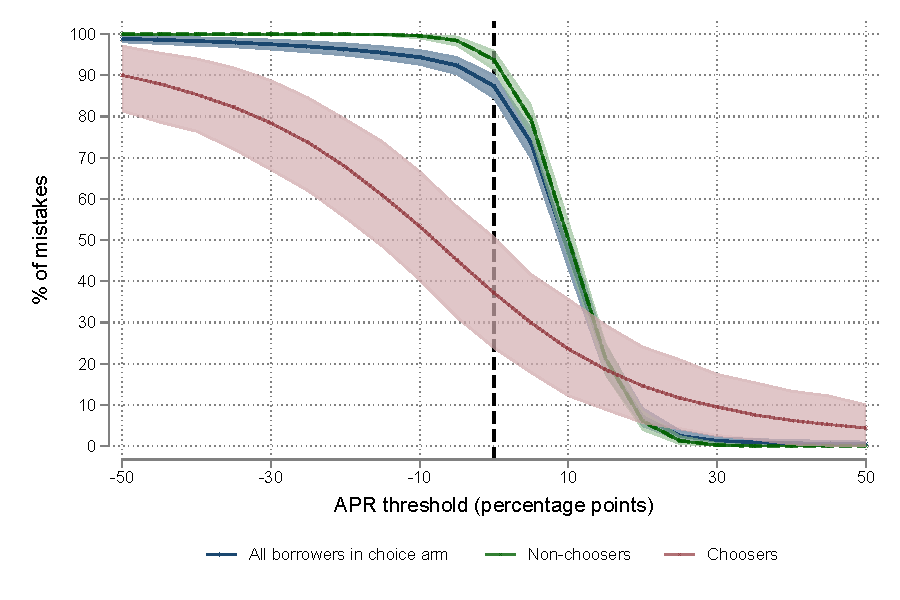
\includegraphics[width=\textwidth]{Figuras/line_cw_apr_tot_tut.pdf}
        
    \end{subfigure}
        \begin{subfigure}{0.45\textwidth}
        \caption{Financial value of mistake}
        \centering
        \includegraphics[width=\textwidth]{Figuras/money_cw_apr_tot_tut.pdf}

    \bigskip
        
    \end{subfigure}
        \begin{subfigure}{0.45\textwidth}
        \caption{\% better when forced to forced commitment}
        \centering
        \includegraphics[width=\textwidth]{Figuras/line_better_forceall_apr_te_cf.pdf}
        
    \end{subfigure}
    %     \begin{subfigure}{0.45\textwidth}
    %     \caption{\footnotesize{Effect of CATE benefit vs predicted take-up}}
    %     \centering
    %     \includegraphics[width=\textwidth]{Figuras/benefit_choice.pdf}% takeuppr_def.pdf 
    % \end{subfigure}
    
    \end{center}
        \scriptsize
        In Panel (a) we estimate what the treatment effect of the commitment contract \textit{would have been} for all subjects in the choice arm if they had been forced into the fee-commitment contract. To do this we proceed in two steps. First, we estimate treatment effects in the forcing arm by comparing the Forced Commitment arm against the status quo arm. We let these effects be heterogeneous as a function of our $x$'s using \cite{atheygrf}'s methodology of causal forests. Second, we extrapolate these treatment effects based on the choice arm using the same $x$'s. Once we have personalized counterfactual treatment effects in the choice arm we calculate what fraction of subjects in the choice arm incurred in financial costs that are  $> z$\% than if they had chosen the opposite contract of what they actually chose, were $z$\% is defined as a fraction of the loan. $z$\% is a level of tolerance we can vary and we plot it in the X-axis. The left Y-axis measures the fraction of subjects that would have been better by a margin of $z$\% if they changed their choice, and the right Y-axis measures the amount of money ``left on the table''. We use bootstrap to tighten the confidence intervals (CIs). \cite{atheygrf}'s heterogeneous treatment effect using GRF is asymptotically normal. We compute the HTE ($\mu$) together with standard errors ($\sigma$) . For every pledge, we draw a random effect from a normal distribution with parameters ($\mu$,$\sigma^2$), and compute via bootstrap the percentage that choose wrong, along normal-approximation CIs (results are robust if we use instead percentile CIs or bias-corrected CIs) . This allows us to estimate a distribution for the upper and lower bound CIs, which we then use to obtain a 95\% CI. Panel (b) is analogous to Panel (a) except that it does the exercise separately for clients we classified as overconfident ($OC_i:=\mathbbm{1}(P^s_i-\widehat{P_i(X_i)}>0))$ and those we classified as not overconfident. Panel (c) simulates what percentage would be better by at least $z$ if we forced everybody of those in the Commitment Choice arm into the fee-commitment contract.
        % Panel (d) asks whether it is the case that people with larger causal benefits from the Forced Commitment contract would be more likely to select that contract. To do this we proceed in two steps as well. First we estimate a flexible model of take-up of the fee commitment contract \textit{in the choice arm} using random forests, and from this model obtain a probability $P(x_i)$ of choosing the Forced Commitment contract for a client with characteristics $x_i$. We extrapolate this model to clients in the Forced Commitment arm to estimate what would they have chosen if we had given them choice. 
        % Figure (d) plots $\widehat{P(x_i)}$ in the X-axis using a binscatter that splits the X-axis in 100 percentile bins. The Y-axis plots the heterogeneous treatment effects of the fee forcing contract on the probability of losing the pawns (more negative means then more likely to recover it), averaged for the respective x-axis bin. Positive assortative selection would mean a negative relationship: those who benefit more by treatment and lose the pawn less are \emph{less} likely to choose it.  Using all bins we estimate a slope of zero in the relationship. Using the 80 right most points, we estimate a \textit{positive} relationship.
        %\textit{Do file: }  \texttt{choose\_wrong\_quant\_wrong.do, choose\_wrong\_quant\_wrong\_decomposition.do}
\end{figure}




\cleardoublepage






    
\begin{figure}[H]
    \caption{Negative selection on treatment effects}
    \label{benefit_vs_choice_cdf}
    \begin{center}
    \begin{subfigure}{0.475\textwidth}
        \caption{APR benefit}
        \centering
        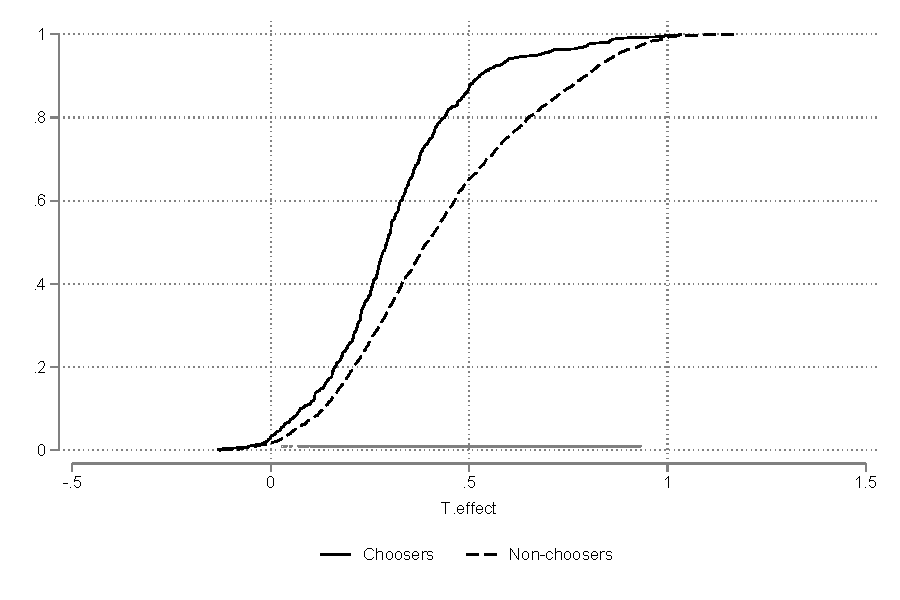
\includegraphics[width=\textwidth]{Figuras/cdf_predchoose_tau_apr.pdf}
    \end{subfigure}
    \begin{subfigure}{0.475\textwidth}
        \caption{Repayment}
        \centering
        \includegraphics[width=\textwidth]{Figuras/cdf_predchoose_tau_des.pdf}
    \end{subfigure}
    \begin{subfigure}{0.475\textwidth}
        \caption{Default}
        \centering
        \includegraphics[width=\textwidth]{Figuras/cdf_predchoose_tau_def.pdf}
    \end{subfigure}
    \end{center}
     \scriptsize    CDF of the heterogeneous treatment effect for choosers vs non-choosers. The dotted line below indicates the points where the difference in the distributions is significant.  Instead of a single global null hypothesis (that the two CDFs are identical), there is a continuum of individual null hypotheses of CDF equality at each point. This methodology was proposed by \cite{GOLDMAN2018143}.
     
     
     \hl{Isaac : If I recall correctly we agreed to not work with the propensities. Besides this is giving us different results(?) - this was due to not using actual choosers and the prop. score model not being very good. Thus this will be removed? }
          %\footnotesize{ \textit{Do file: }  \texttt{benefit\_choice.do}}
\end{figure}

















\newpage
%  \documentclass[oneside,11pt]{article}

% 
\usepackage{soul}
\usepackage{natbib}
\usepackage{hyperref}
\usepackage{graphicx}             
\graphicspath{{./Figuras/}}

\usepackage{makecell}
\usepackage[margin=1.0in]{geometry}
\usepackage{float}                
\usepackage{amsmath}
\usepackage{amscd}
\usepackage{amsfonts}
\usepackage{amssymb}
\usepackage{bbm}
\usepackage{booktabs}
\usepackage{nameref}
\usepackage{multirow}
\usepackage[nokeyprefix]{refstyle}
\usepackage{rotating}
\usepackage{threeparttable}
\usepackage{lscape}
\usepackage{enumerate}
\usepackage{afterpage}
\usepackage{caption}
\usepackage{subcaption}
\usepackage{epstopdf}
\epstopdfDeclareGraphicsRule{.tiff}{png}{.png}{convert #1 \OutputFile}
\AppendGraphicsExtensions{.tiff}

\epstopdfDeclareGraphicsRule{.tif}{png}{.png}{convert #1 \OutputFile}
\AppendGraphicsExtensions{.tif}

\usepackage{tikz}
\usetikzlibrary{shapes.geometric, arrows}
\usetikzlibrary{calc}
\usetikzlibrary{matrix}

\tikzset{ 
    table/.style={
        matrix of nodes,
        row sep=-\pgflinewidth,
        column sep=-\pgflinewidth,
        nodes={
            rectangle,
            draw=black,
            align=center
        },
        minimum height=1.5em,
        text depth=0.5ex,
        text height=2ex,
        nodes in empty cells,
%%
        every even row/.style={
            nodes={fill=gray!20}
        },
        column 1/.style={
            nodes={text width=2em,font=\bfseries}
        },
        row 1/.style={
            nodes={
                fill=black,
                text=white,
                font=\bfseries
            }
        }
    }
}


\usepackage{colortbl}

\newtheorem{theorem}{Theorem}
\newtheorem{claim}[theorem]{Claim}



% %%% HELPER CODE FOR DEALING WITH EXTERNAL REFERENCES
% \usepackage{xr}
% \makeatletter
% \newcommand*{\addFileDependency}[1]{
%   \typeout{(#1)}
%   \@addtofilelist{#1}
%   \IfFileExists{#1}{}{\typeout{No file #1.}}
% }
% \makeatother


% \newcommand*{\myexternaldocument}[1]{
%     \externaldocument{#1}
%     \addFileDependency{#1.tex}
%     \addFileDependency{#1.aux}
% }

% %\myexternaldocument{OA}

% %%%%%%%%%%%%%%%%%%%%%%%%%%%%%%%% DOCUMENT
% \begin{document}

%%%%%%%%%%%%%%%%%%%%%%%%%%%%%%%%%%%%%%%%%%%%%%%

% APPENDIX 
\setcounter{table}{0}
\setcounter{figure}{0}
\setcounter{section}{0}
\pagenumbering{gobble}


\begin{center}
	\LARGE The limits of self-commitment and private paternalism \\[0.5em]
	\Large{Appendix $-$ For Online Publication} \\[1em]
	\large \author{Craig McIntosh \and Isaac Meza \and Joyce Sadka \and Enrique Seira}
\end{center}

\appendix
\pagenumbering{arabic}
\renewcommand\thefigure{OA-\arabic{figure}}
\renewcommand\thetable{OA-\arabic{table}}
\renewcommand*{\thepage}{OA - \arabic{page}}
\renewcommand\thesection{Appendix \Alph{section}.}
\renewcommand\thesubsection{\Alph{section}.\arabic{subsection}}

%\renewcommand{\cftparskip}{0em} % NOT NEEDED
\renewcommand\cftsecdotsep{\cftdotsep}
\renewcommand\cftsubsecdotsep{\cftnodots}
\renewcommand{\cftsecnumwidth}{6em}
 \renewcommand{\cftpnumalign}{r}
%\renewcommand{\cftsecleader}{\normalfont\cftdotfill{\cftsecdotsep}}


\renewcommand{\cftsecleader}{\cftdotfill{\cftsecdotsep}\hspace{1.8em}}
%\renewcommand{\cftsecpagefont}{20em}
%\renewcommand{\cftfignumwidth}{6em}
%\renewcommand{\cfttabnumwidth}{3.3em}

%\tableofcontents
\etocdepthtag.toc{mtappendix}
\etocsettagdepth{mtchapter}{none}
\etocsettagdepth{mtappendix}{subsection}

\setstretch{0.9}
%\renewcommand\contentsname{} % the empty name

\begingroup
\let\clearpage\relax
%\vspace{-1.5em} % the removed space. Set as appropriate
\tableofcontents
\endgroup


\newpage



\section{ }
\vspace{.2in}




\vspace{.1in}


\begin{figure}[H]
     \caption{Some Pawnshops}
    \label{PawnshopPicture}
    \begin{center}
    \begin{subfigure}{0.42\textwidth}
    \caption{Appraiser/tellers inside a pawnshop}
        \centering
        \includegraphics[width=\textwidth]{Figuras/empenio9.png}
    \end{subfigure}
        \begin{subfigure}{0.45\textwidth}
    \caption{Pawnshop}
        \centering
        \includegraphics[width=\textwidth]{Figuras/empenio11.png}
    \end{subfigure}
    
        \vspace{3ex}

    \begin{subfigure}{0.45\textwidth}
    \caption{Pawnshop}
        \centering
        \includegraphics[width=\textwidth]{Figuras/empenio2.png}
    \end{subfigure}
    \begin{subfigure}{0.42\textwidth}
    \caption{Lost pawns which are for sale}
        \centering
        \includegraphics[width=\textwidth]{Figuras/empenio3.png}
    \end{subfigure}
    \end{center}
    \scriptsize
        This figure  shows pictures of pawnshops in Mexico city. They do not necessarily coincide with Lender P for confidentiality. 
\end{figure}



\vspace{.1in}
\begin{figure}[H]
     \caption{Gold buyers next to pawnshops}
    \label{GoldBuyers}
    \begin{center}
    \begin{subfigure}{.49\textwidth}
    \caption{Gold buyer next to pawnshop 1}
        \centering
        \includegraphics[width=\textwidth]{Figuras/empenio7.png}
    \end{subfigure}
    \begin{subfigure}{.49\textwidth}
    \caption{Gold buyer next to pawnshop 1}
        \centering
        \includegraphics[width=\textwidth]{Figuras/empenio8.png}
    \end{subfigure}
       \vspace{3ex}
       
    \end{center}
    \scriptsize
        This figure shows pictures of gold buyers next to pawnshops in Mexico city. They do not necessarily coincide with Lender P for confidentiality. 
\end{figure}




\begin{table}[H]
\caption{Number of pawns balance before and after the experiment}
\label{num_pawns_bal}
\begin{center}
\scriptsize{% Table generated by Excel2LaTeX from sheet 'num_pawns_bal'
\begin{tabular}{lcccc}
\toprule
      & \multicolumn{4}{c}{Pawns per day} \\
\midrule
      & 0-degree & 1-degree & 2-degree & 3-degree \\
\midrule
\midrule
      & (1)   & (2)   & (3)   & (4) \\
\midrule
\midrule
$\beta_a$ & 2.48  & -3.32 & -0.65 & -0.65 \\
      & (1.36) & (1.85) & (2.80) & (2.80) \\
$\beta_b$ & 0.20  & 1.82  & 1.32  & 1.32 \\
      & (0.97) & (0.93) & (0.67) & (0.67) \\
      &       &       &       &  \\
\midrule
Observations & 628   & 628   & 628   & 628 \\
R-sq  & 0.737 & 0.747 & 0.747 & 0.747 \\
Branch FE & \checkmark & \checkmark & \checkmark & \checkmark \\
\bottomrule
\bottomrule
\end{tabular}%
}
\end{center}
 \scriptsize 
%\textit{Do file: } \texttt{num\_pawns\_bal.do}
\end{table}



\subsection{Surveys}

\afterpage{
\begin{table}[H]
\caption{Baseline survey}
\label{baseline_survey}
\begin{center}
\scriptsize{% Table generated by Excel2LaTeX from sheet 'transcribed'
\begin{tabular}{cl}
\toprule
      & \textbf{Baseline Survey} \\
\midrule
\midrule
1     & \textbf{Your pawn was:} \\
      & (a) Inherite, (b) a gift, (c) bought by me, (d) lend to me, (e) other \_\_\_\_\_\_\_\_\_\_\_\_ \\
2     & \textbf{Mark with an "X" in the line below how likely is that you recover your pawn. } \\
      & \textbf{Where 0 is impossible and 100 is completely certain} \\
3     & \textbf{How much would you sell the item you want to pawn for?       \_\_\_\_\_\_\_\_\_\_\_\_\_\_ pesos} \\
4     & \textbf{Gender      } \\
5     & \textbf{Age} \\
6     & \textbf{Civil Status } \\
      & (a) married, (b) single, (c) divorced, (d) widowed \\
7     & \textbf{Work status} \\
      & (a) employed, (b) own business, (c) houseshores, (d) don't work, (e) retired, (f) study \\
8     & \textbf{Education} \\
      & (a) no formal education, (b) primary, (c) middle school, (d) highschool, (e) more than highschool \\
9     & \textbf{In the last month, did a friend or family member asked you for money?} \\
      & (a) yes  (b) no \\
10    & \textbf{What would you like to have: 100 pesos tomorrow or 150 pesos in one month?} \\
11    & \textbf{How often do you feel stressed by your economic situation?} \\
      & (a) always, (b) very often, (c) sometimes, (d) never \\
12    & \textbf{What is the main reason you want to pawn?} \\
      & (a) Need the money because somebody in my family lost his/her job \\
      & (b) Need the money to pay for a sickness in the family \\
      & (c) Need the money for an urgent expense \\
      & (d) Need the money for some non urgent expense. \\
13    & \textbf{How stressed do you feel from the situation that led to to pawn?} \\
      & (a) very stressed, (b) somwhat stressed, (c) a little stressed, (d) not stressed  \\
14    & \textbf{In 3 months, I expect to have a  \_\_\_\_\_\_\_\_\_\_\_\_\_\_\_\_ situation} \\
      & (a) better, (b) similar,  (c) worse \\
15    & \textbf{Have you panwned before?} \\
      & (a) yes  (b) no \\
16    & \textbf{How many times have you pawned on a Lender P branch?} \\
      & (a) NO\_\_\_    (b)  1-2 times \_\_\_    (c) 3-5 times\_\_\_\_   (d) More than 5\_\_\_\_ \\
17    & \textbf{If you are saving money and a family member wants to use it for something } \\
      & (a) I would only give him the money for an urgent expenze \\
      & (b) I would give him the money even if it was not an urgent expense \\
      & (c) I would not give him/her the money regardless \\
      & (d) No one would ask me for my money \\
18    & \textbf{Do you make an expenses budget for the month ahead of time?} \\
      & (a) always, (b) very often, (c) sometimes, (d) never \\
19    & \textbf{Do you have other items you could pawn?} \\
      & (a) yes  (b) no \\
20    & \textbf{Do you have savings?} \\
      & (a) yes  (b) no \\
21    & \textbf{Do you participate in a ROSCA?} \\
      & (a) yes  (b) no \\
22    & \textbf{Is it common that family or friends ask for money?} \\
      & (a) yes  (b) no \\
23    & \textbf{How much did you spend to come to the branch today?    \$\_\_\_\_\_\_\_\_\_\_\_\_\_\_ pesos} \\
24    & \textbf{How much time does it usually take to come to this branch?    \_\_\_\_\_\_\_\_\_\_\_} \\
25    & \textbf{How much does your family spend in a normal week?   \$\_\_\_\_\_\_\_\_\_\_\_\_\_\_ pesos} \\
26    & \textbf{How much do you manage to save in a normal week?   \$\_\_\_\_\_\_\_\_\_\_\_\_\_\_ pesos} \\
27    & \textbf{Does it happen to you that you spend more than you wanted because you fall into temptation?} \\
      & (a) never, (b) almost never, (c) sometimes, (d) very often \\
28    & \textbf{In the last 6 months, has it happened that at some point you lacked money to pay} \\
      & (a) rent?    (b) food    (c)food   (d) medicine  (e) electricity   (f) heating   (g) telephone    (i) water \\
29    & \textbf{What would you like to have: 100 pesos in 3 months or 150 pesos in four months?} \\
30    & \textbf{Would you like to receive (free) reminders for upcomming payments?} \\
      & (a) yes  (b) no \\
\bottomrule
\end{tabular}%
}
\end{center}
\end{table}
}


\begin{table}[H]
\caption{Balance table conditional on survey \& response rates}
\label{SS_cond_survet}
\begin{center}
\scriptsize{% Table generated by Excel2LaTeX from sheet 'SS_cond_survey'
\begin{tabular}{lcccc}
\toprule
      &       & \multicolumn{3}{c}{Commitment arms} \\
\cmidrule{3-5}      & \multicolumn{1}{p{4.5em}}{Control} & \multicolumn{1}{p{4.93em}}{Forced} & \multicolumn{1}{p{3.43em}}{Choice} & \multicolumn{1}{p{3.43em}}{p-value} \\
\midrule
      & \multicolumn{4}{c}{Panel A : Administrative Data (conditional on survey)} \\
\midrule
\midrule
Loan amount  & 2199  & 2196  & 2216  & 0.98 \\
      & (86)  & (106) & (81)  &  \\
Weekday & 0.88  & 0.89  & 0.85  & 0.8 \\
      & (0.045) & (0.038) & (0.045) &  \\
\midrule
Obs   & 1386  & 1469  & 1982  &  \\
\midrule
      & \multicolumn{4}{c}{Panel B : Survey Data - response rate} \\
\midrule
\midrule
Subjective value & 0.73  & 0.69  & 0.71  & 0.39 \\
      & (0.022) & (0.024) & (0.024) &  \\
Trouble paying bills & 0.49  & 0.48  & 0.44  & 0.29 \\
      & (0.023) & (0.022) & (0.022) &  \\
Present bias & 0.43  & 0.44  & 0.39  & 0.17 \\
      & (0.02) & (0.02) & (0.02) &  \\
Makes budget & 0.55  & 0.56  & 0.53  & 0.56 \\
      & (0.023) & (0.023) & (0.019) &  \\
Subj. pr. of recovery & 0.74  & 0.72  & 0.74  & 0.71 \\
      & (0.024) & (0.025) & (0.025) &  \\
Pawn before & 0.55  & 0.57  & 0.53  & 0.57 \\
      & (0.023) & (0.024) & (0.02) &  \\
Age   & 0.54  & 0.55  & 0.52  & 0.59 \\
      & (0.023) & (0.023) & (0.018) &  \\
Woman & 0.58  & 0.59  & 0.58  & 0.93 \\
      & (0.025) & (0.024) & (0.02) &  \\
+ High-school & 0.54  & 0.55  & 0.51  & 0.39 \\
      & (0.025) & (0.025) & (0.019) &  \\
\midrule
Obs   & 1386  & 1469  & 1982  &  \\
\bottomrule
\bottomrule
\end{tabular}%
}
\end{center}

%\textit{Do file: } \texttt{ss\_att.do}
\end{table}


\newpage
\subsection{Some more evidence of overconfidence}

\vspace{.2in}
\begin{figure}[H]
    \caption{Behavior of those who lost pawn}
    \label{proxy_naive}
    \begin{center}
    \begin{subfigure}{0.40\textwidth}
        \caption{Elapsed days to first payment}
        \centering
        \includegraphics[width=\textwidth]{Figuras/hist_firstdays_default.pdf}
    \end{subfigure}
    \begin{subfigure}{0.40\textwidth}
        \caption{Elapsed days to last payment}
        \centering
        \includegraphics[width=\textwidth]{Figuras/hist_days_default.pdf}
    \end{subfigure}
        \begin{subfigure}{0.40\textwidth}
        \caption{Payments as \% of loan}
        \centering
        \includegraphics[width=\textwidth]{Figuras/hist_percpay_default.pdf}
    \end{subfigure}
    \begin{subfigure}{0.40\textwidth}
        \caption{Number of payments}
        \centering
        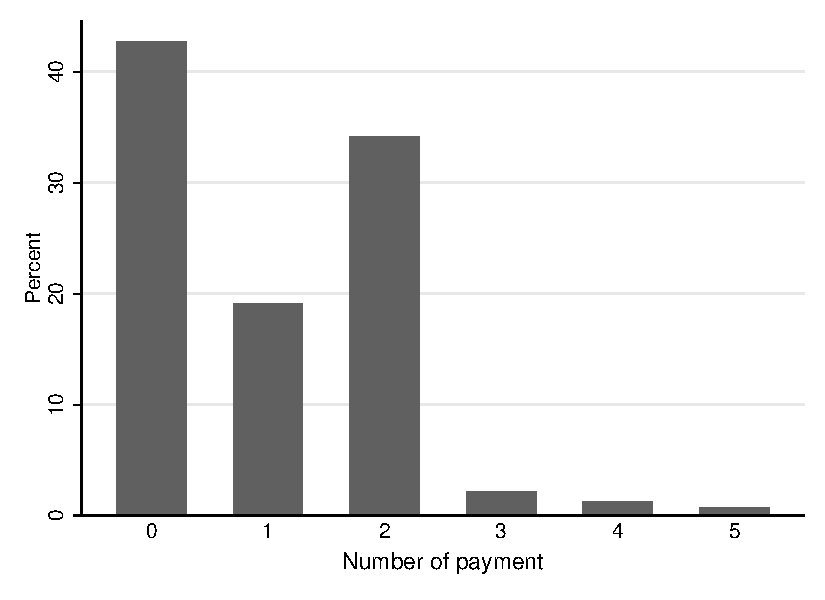
\includegraphics[width=\textwidth]{Figuras/hist_numpay_default.pdf}
    \end{subfigure}
    \end{center}
        \scriptsize 
        This figure describes behavior for the subsample of clients whose pawn was not recovered (in the control group).  Panel (a) shows days elapsed from the pawn to the first payment, while panel (b) displays the days elapsed to last payment. Some people pay after the day 105 when the grace period ends because the can ``restart'' the loan if they pay all interest owed. It amounts to starting a new loan with the same conditions and same pawn. Panel (c) shows the fraction of the loan that they paid (even when they ended up losing the pawn). Panel (d) displays the number of times they went to the branch to pay.      
      %\textit{Do file: }  \texttt{hist\_den\_default.do}
\end{figure}


\newpage
\subsection{Main treatment effects: Additional material}

\begin{table}[H]
\caption{Bounding censoring}
\label{bounding_censoring}
\begin{center}
\resizebox{0.9\textwidth}{!}{
\scriptsize{% Table generated by Excel2LaTeX from sheet 'censoring_imp'
\begin{tabular}{lcccccc}
\toprule
      & FC    & Interest pymnt & Principal pymnt & Lost pawn value & Default & APR \\
\midrule
      & \multicolumn{6}{c}{Panel A : $\quad$ Control  = 0           $\quad\quad$                  Forced Commitment = 0} \\
\midrule
\midrule
      & (1)   & (2)   & (3)   & (4)   & (5)   & (6) \\
\midrule
\midrule
Forced commitment  & -408.3*** & -191.8*** & -0.42 & -248.1** & -0.063*** & -0.37*** \\
      & (107.2) & (37.6) & (3.01) & (101.4) & (0.023) & (0.078) \\
      &       &       &       &       &       &  \\
\midrule
Observations & 3724  & 3724  & 3724  & 3724  & 3724  & 3724 \\
R-sq  & 0.012 & 0.025 & 0.004 & 0.012 & 0.019 & 0.022 \\
Control Mean & 1898.1 & 593.5 & 5.75  & 1304.7 & 0.43  & 1.88 \\
\midrule
\midrule
      &       &       &       &       &       &  \\
\midrule
      & \multicolumn{6}{c}{Panel B : $\quad$ Control  = 0         $\quad\quad$                    Forced Commitment = 1} \\
\midrule
\midrule
      & (7)   & (8)   & (9)   & (10)  & (11)  & (12) \\
\midrule
\midrule
Forced commitment  & -226.1** & -207.7*** & 1.38  & -50.0 & 0.0094 & 0.095 \\
      & (110.8) & (37.4) & (3.45) & (103.3) & (0.024) & (0.096) \\
      &       &       &       &       &       &  \\
\midrule
Observations & 3724  & 3724  & 3724  & 3724  & 3724  & 3724 \\
R-sq  & 0.009 & 0.026 & 0.004 & 0.009 & 0.014 & 0.014 \\
Control Mean & 1898.1 & 593.5 & 5.75  & 1304.7 & 0.43  & 1.88 \\
\midrule
\midrule
      &       &       &       &       &       &  \\
\midrule
      & \multicolumn{6}{c}{Panel C : $\quad$ Control  = 1        $\quad\quad$                     Forced Commitment = 0} \\
\midrule
\midrule
      & (13)  & (14)  & (15)  & (16)  & (17)  & (18) \\
\midrule
\midrule
Forced commitment  & -804.2*** & -140.4*** & -2.33 & -695.5*** & -0.21*** & -1.17*** \\
      & (113.3) & (34.1) & (3.16) & (100.8) & (0.023) & (0.10) \\
      &       &       &       &       &       &  \\
\midrule
Observations & 3724  & 3724  & 3724  & 3724  & 3724  & 3724 \\
R-sq  & 0.022 & 0.020 & 0.004 & 0.022 & 0.053 & 0.082 \\
Control Mean & 2272.4 & 545.9 & 7.69  & 1726.5 & 0.57  & 2.62 \\
\midrule
\midrule
      &       &       &       &       &       &  \\
\midrule
      & \multicolumn{6}{c}{Panel D : $\quad$ Control  = 1       $\quad\quad$                      Forced Commitment = 1} \\
\midrule
\midrule
      & (19)  & (20)  & (21)  & (22)  & (23)  & (24) \\
\midrule
\midrule
Forced commitment  & -622.0*** & -156.3*** & -0.53 & -497.3*** & -0.13*** & -0.71*** \\
      & (117.3) & (33.8) & (3.58) & (103.1) & (0.024) & (0.12) \\
      &       &       &       &       &       &  \\
\midrule
Observations & 3724  & 3724  & 3724  & 3724  & 3724  & 3724 \\
R-sq  & 0.015 & 0.021 & 0.003 & 0.013 & 0.028 & 0.030 \\
Control Mean & 2272.4 & 545.9 & 7.69  & 1726.5 & 0.57  & 2.62 \\
\midrule
\midrule
      &       &       &       &       &       &  \\
\midrule
      & \multicolumn{6}{c}{Panel E : $\quad$ Prediction with lasso-logit model} \\
\midrule
\midrule
      & (25)  & (26)  & (27)  & (28)  & (29)  & (30) \\
\midrule
\midrule
Forced commitment  & -529.7*** & -172.4*** & -1.26 & -389.4*** & -0.12*** & -0.62*** \\
      & (120.5) & (37.4) & (3.22) & (110.2) & (0.025) & (0.11) \\
Choice commitment & -61.5 & -30.6 & -4.52 & -32.3 & -0.016 & -0.039 \\
      & (124.6) & (42.0) & (2.78) & (114.5) & (0.023) & (0.11) \\
      &       &       &       &       &       &  \\
\midrule
Observations & 6304  & 6304  & 6304  & 6304  & 6304  & 6304 \\
R-sq  & 0.012 & 0.022 & 0.003 & 0.009 & 0.016 & 0.024 \\
Control Mean & 2077.4 & 567.5 & 7.51  & 1509.9 & 0.51  & 2.28 \\
\bottomrule
\bottomrule
\end{tabular}%
}
}
\end{center}
 \scriptsize 
%\textit{Do file: } \texttt{censoring_imp.do, censoring_imp_pr.do}
\end{table}

\begin{figure}[H]
        \caption{Interpolation on bounding censoring}
    \label{interpolation_censoring_imp}
    \begin{center}
   \begin{subfigure}{0.49\textwidth}
   \caption{Significance area for Default }
        \centering
        \includegraphics[width=\textwidth]{Figuras/frontera_sig_def_imp.pdf}
    \end{subfigure} 
   \begin{subfigure}{0.49\textwidth}
   \caption{Significance area for APR}
        \centering
        \includegraphics[width=\textwidth]{Figuras/frontera_sig_apr.pdf}
    \end{subfigure}     
    \end{center}
     \scriptsize  The next figure aims to answer the following question: For how many loans in the control arm can we impute recovery, and for how many in the treatment arm can we impute default and still have significance?
     This figure shows exactly the boundary separating significance when we vary the percentage of imputed censored loans with recovery and default respectively for control and treatment. Each corner in the square will correspond to one of the panels from the Table \ref{bounding_censoring}. For instance, the origin is the best-case scenario (Panel C) and the point (100,100) (Panel D) is the worst-case scenario. Thus we can think of this graph as an `interpolation' from the four extreme cases. The `x' indicates the proportions imputed by the lasso-logit model, and the different lines correspond to setting different significance levels. 

     %\textit{Do file: }  \texttt{interpolation_{censoring_imp.do}
\end{figure}






\begin{figure}[H]
        \caption{Financial cost TUT effect for different discount rates}
    \label{fc_discount_rates}
    \begin{center}
        \centering
        \includegraphics[width=0.55\textwidth]{Figuras/discount_effect_tut.pdf}
    \end{center}
     \scriptsize This Figure estimates the treatment effect on financial cost for the untreated with different discount rates.  
     %\textit{Do file: }  \texttt{discounted\_noeffect.do}
\end{figure}





\begin{figure}[H]
    \caption{Partition of TuT \& ToT effect by behavioral variables.}
    \label{tut_beh_partition}
    \begin{center}
    \begin{subfigure}{0.475\textwidth}
        \caption{TuT}
        \centering
        \includegraphics[width=\textwidth]{Figuras/tut_beh_partition.pdf}
    \end{subfigure}
    \begin{subfigure}{0.475\textwidth}
        \caption{ToT}
        \centering
        \includegraphics[width=\textwidth]{Figuras/tot_beh_partition.pdf}
    \end{subfigure}
  
    \end{center}
     \scriptsize    \\
      %\footnotesize{ \textit{Do file: }  \texttt{partition_tot_tut.do}
\end{figure}




\cleardoublepage

\begin{landscape}

\begin{table}[H]
\caption{Multiple-loans robustness check}
\label{multiple_loans}
\begin{center}
\scriptsize{% Table generated by Excel2LaTeX from sheet 'multiple_loans'
\begin{tabular}{lcccccccccccccc}
\toprule
      & \multicolumn{4}{c}{First visit (Baseline approach)} &       & \multicolumn{4}{c}{Multiple visits - multiple treatments} &       & \multicolumn{4}{c}{First treatment (ITT)} \\
\cmidrule{7-10}\cmidrule{12-15}      & FC    & APR   & Recovery & Default &       & FC    & APR   & Recovery & Default &       & FC    & APR   & Recovery & Default \\
\midrule
      & (1)   & (2)   & (3)   & (4)   &       & (5)   & (6)   & (7)   & (8)   &       & (9)   & (10)  & (11)  & (12) \\
\midrule
\midrule
Forced Commitment & -202.8*** & -0.11*** & 0.14*** & -0.065*** &       & -175.2*** & -0.078*** & 0.099*** & -0.032 &       & -159.1*** & -0.086*** & 0.11*** & -0.051*** \\
      & (48.1) & (0.019) & (0.025) & (0.023) &       & (42.8) & (0.017) & (0.021) & (0.020) &       & (38.6) & (0.015) & (0.021) & (0.019) \\
Choice Commitment & -39.6 & -0.0089 & 0.0094 & -0.024 &       & -34.4 & 0.0028 & 0.00054 & -0.0049 &       & -31.5 & -0.017 & 0.029 & -0.032* \\
      & (49.8) & (0.019) & (0.022) & (0.021) &       & (43.5) & (0.016) & (0.018) & (0.018) &       & (40.4) & (0.014) & (0.018) & (0.018) \\
      &       &       &       &       &       &       &       &       &       &       &       &       &       &  \\
\midrule
Observations & 6304  & 6304  & 6304  & 6304  &       & 8519  & 8519  & 8519  & 8519  &       & 8813  & 8813  & 8813  & 8813 \\
R-sq  & 0.013 & 0.031 & 0.019 & 0.013 &       & 0.016 & 0.032 & 0.018 & 0.010 &       & 0.016 & 0.031 & 0.020 & 0.015 \\
Control Mean & 941.3 & 0.57  & 0.43  & 0.44  &       & 905.7 & 0.54  & 0.46  & 0.42  &       & 904.7 & 0.55  & 0.44  & 0.44 \\
\bottomrule
\bottomrule
\end{tabular}%
}
\end{center}
 \scriptsize

%\textit{Do file: } \texttt{multiple\_loans.do}
\end{table}

\end{landscape}


\begin{figure}[H]
        \caption{Survival graph}
    \label{survival_graph}
    \begin{center}
   \begin{subfigure}{0.49\textwidth}
   \caption{Ended contract}
        \centering
        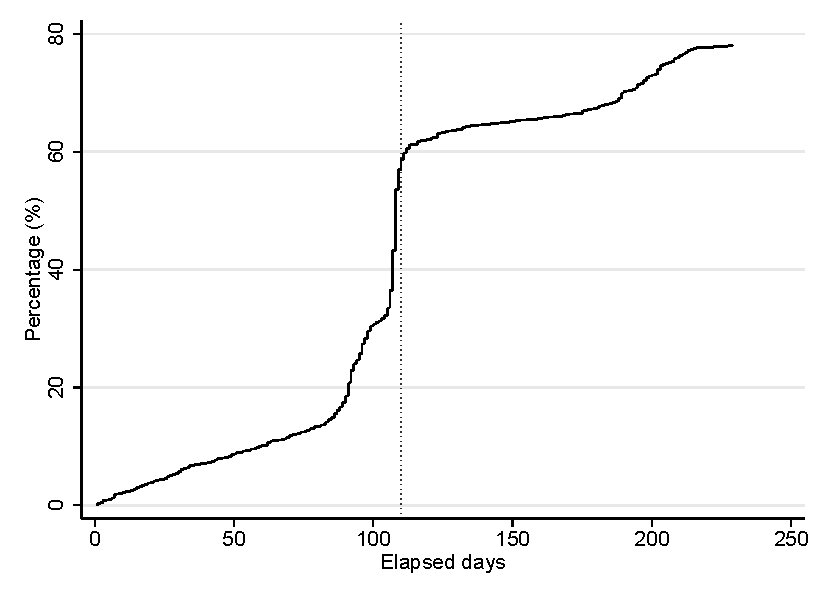
\includegraphics[width=\textwidth]{Figuras/survival_graph_ended.pdf}
    \end{subfigure} 
   \begin{subfigure}{0.49\textwidth}
   \caption{Recovery}
        \centering
        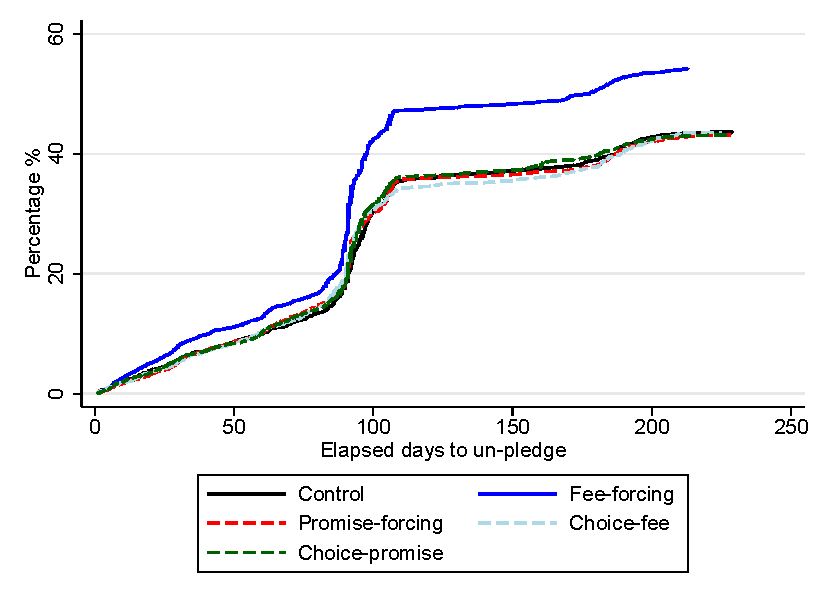
\includegraphics[width=\textwidth]{Figuras/survival_graph_unpledge.pdf}
    \end{subfigure}     
    \end{center}
     \scriptsize  This Figure shows the accumulated percentage of recovery in time by treatment arm. 
     %\textit{Do file: }  \texttt{survival\_graph.do}
\end{figure}

\begin{figure}[H]
        \caption{\% of payment over time}
    \label{porc_payment_over_time}
    \begin{center}
   \begin{subfigure}{0.49\textwidth}
        \caption{Unconditional}
        \centering
        \includegraphics[width=\textwidth]{Figuras/cumulative_porc_pay_time.pdf}
    \end{subfigure} 
   \begin{subfigure}{0.49\textwidth}
        \caption{Conditional on default}
        \centering
        \includegraphics[width=\textwidth]{Figuras/cumulative_porc_pay_time_default.pdf}
    \end{subfigure}     
    \end{center}
     \scriptsize  This Figure shows the accumulated percentage of recovery in time by treatment arm. 
     %\textit{Do file: }  \texttt{cumulative\_porc\_pay\_time.do}
\end{figure}






\cleardoublepage


\vspace{.2in}
\begin{figure}[H]
        \caption{Empirical CDF of Financial Cost: fee-focing vs status-quo}
    \label{ecdf_fc}
    \begin{center}
        \centering
        \includegraphics[width=0.65\textwidth]{Figuras/cdf_fc_pro_2.pdf}
    \end{center}
    \scriptsize This figure plots the empirical cumulative distribution of financial cost. It does this separately for the fee-forcing contract and for the status-quo contract. The doted line at the bottom is the difference of the status-quo CDF minus the fee-forcing CDF. It shows that the CDF of the status quo contract is always below that of the fee-forcing (and this difference is significant for the points indicated by the blue line), and therefore that the former first-order stochastically dominates the later for weakly decreasing utility functions; see Proposition \ref{eq_fosd}.
    % \texttt{ecdf\_fc.do}}
\end{figure}

\begin{figure}[H]
        \caption{Empirical CDF of APR: fee-focing vs status-quo}
    \label{ecdf_fc}
    \begin{center}
        \centering
        \includegraphics[width=0.65\textwidth]{Figuras/cdf_eff_pro_2.pdf}
    \end{center}
    \scriptsize This figure plots the empirical cumulative distribution of financial cost. It does this separately for the fee-forcing contract and for the status-quo contract. The doted line at the bottom is the difference of the status-quo CDF minus the fee-forcing CDF. It shows that the CDF of the status quo contract is always below that of the fee-forcing (and this difference is significant for the points indicated by the blue line), and therefore that the former first-order stochastically dominates the later for weakly decreasing utility functions; see Proposition \ref{eq_fosd}.
    % \texttt{ecdf\_eff.do}}
\end{figure}


\vspace{.2in}
\begin{table}[H]
\caption{Clients who should prefer fee-forcing financial cost distribution}
\label{stochastic_dominance}
\begin{center}
\scriptsize{% Table generated by Excel2LaTeX from sheet 'dominance'
\begin{tabular}{lccc}
\toprule
Sub-population & Dominance & Log-normality (AD/KS) & Obs \\
\midrule
\midrule
Fee-forcing & \cellcolor[rgb]{ .557,  .663,  .859} $\succeq_{1}^*$ & */*  |  */* & 5034 \\
Low-loan & $\succeq_{1}^*$ &    /     |     /    & 2508 \\
High-loan & $\succeq_{1}^*$ &    /     |     /    & 2526 \\
Low-subj. prob. & \cellcolor[rgb]{ .557,  .663,  .859} $\succeq_{1}^*$ & */*  |  */* & 1083 \\
High-subj. Prob. & \cellcolor[rgb]{ .557,  .663,  .859} $\succeq_{1}^*$ & */*  |  */* & 2590 \\
Low-age & $\preceq_{1}$ & */*  |  */* & 1358 \\
High-age & \cellcolor[rgb]{ .851,  .882,  .949} $\succeq_{1}$ & */*  |     /* & 1363 \\
Low-income index & \cellcolor[rgb]{ .851,  .882,  .949} $\succeq_{1}$ & */*  |  */* & 1047 \\
High-income index & \cellcolor[rgb]{ .851,  .882,  .949} $\succeq_{1}$ & */*  |  */* & 948 \\
Male  & -     & */*  |     /* & 756 \\
Female & \cellcolor[rgb]{ .851,  .882,  .949} $\succeq_{1}$ & */*  |  */* & 2158 \\
First time & $\preceq_{1}$ & */*  |  */* & 293 \\
Pawn before & \cellcolor[rgb]{ .851,  .882,  .949} $\succeq_{1}$ & */*  |  */* & 2476 \\
Family doesn't ask & $\preceq_{1}$ & */*  |  */* & 1826 \\
Family asks & \cellcolor[rgb]{ .557,  .663,  .859} $\succeq_{1}^*$ & */*  |  */* & 988 \\
Not common ask & \cellcolor[rgb]{ .851,  .882,  .949} $\succeq_{1}$ & */*  |  */* & 1436 \\
Common asks & -     & */*  |  */* & 625 \\
No savings & $\preceq_{1}$ & */*  |  */* & 1353 \\
Has savings & \cellcolor[rgb]{ .557,  .663,  .859} $\succeq_{1}^*$ & */*  |  */* & 717 \\
Not rosca & \cellcolor[rgb]{ .557,  .663,  .859} $\succeq_{1}^*$ & */*  |  */* & 1270 \\
Rosca & $\preceq_{1}$ & */*  |  */* & 795 \\
Low-education & \cellcolor[rgb]{ .851,  .882,  .949} $\succeq_{1}$ & */*  |     /* & 906 \\
High-education & \cellcolor[rgb]{ .851,  .882,  .949} $\succeq_{1}$ & */*  |  */* & 1798 \\
Not stressed & -     & */*  |  */* & 1999 \\
Stressed & -     & */*  |  */* & 839 \\
Not overconfident & \cellcolor[rgb]{ .557,  .663,  .859} $\succeq_{1}^*$ & */*  |  */* & 68 \\
Overconfident & \cellcolor[rgb]{ .851,  .882,  .949} $\succeq_{1}$ & */*  |     /* & 1605 \\
Not PB & \cellcolor[rgb]{ .851,  .882,  .949} $\succeq_{1}$ & */*  |  */* & 1438 \\
PB    & \cellcolor[rgb]{ .557,  .663,  .859} $\succeq_{1}^*$ & */*  |     /* & 226 \\
Not FB & \cellcolor[rgb]{ .851,  .882,  .949} $\succeq_{1}$ & */*  |  */* & 1521 \\
FB    & \cellcolor[rgb]{ .851,  .882,  .949} $\succeq_{1}$ & */*  |  */* & 143 \\
Doesn't make budget & \cellcolor[rgb]{ .851,  .882,  .949} $\succeq_{1}$ & */*  |  */* & 1055 \\
Makes budget & \cellcolor[rgb]{ .851,  .882,  .949} $\succeq_{1}$ & */*  |  */* & 1689 \\
Not tempted & \cellcolor[rgb]{ .851,  .882,  .949} $\succeq_{1}$ & */*  |     /* & 875 \\
Tempted & \cellcolor[rgb]{ .851,  .882,  .949} $\succeq_{1}$ & */*  |  */* & 1873 \\
High-transp. cost & \cellcolor[rgb]{ .851,  .882,  .949} $\succeq_{1}$ & */*  |  */* & 1353 \\
Low-transp. cost & \cellcolor[rgb]{ .851,  .882,  .949} $\succeq_{1}$ & */*  |  */* & 1343 \\
High-transp. time & \cellcolor[rgb]{ .851,  .882,  .949} $\succeq_{1}$ & */*  |  */* & 1260 \\
Low-transp. time & \cellcolor[rgb]{ .557,  .663,  .859} $\succeq_{1}^*$ & */*  |  */* & 1443 \\
\bottomrule
\bottomrule
\end{tabular}%
}
\end{center}
 \footnotesize
This table does two things. First, it tests whether the observed empirical distribution of financial cost is well approximated by a log normal. It does this using two tests, the Anderson-Darling and the Kolmogorov-Smirnoff tests. Second, it fits a log normal distribution by maximum likelihood to observed empirical distribution of financial cost, separately for the fee-forcing arm and the status-quo arm. Using the fitted log normal, it tests whether the fee-forcing financial cost distribution would be preferred by any expected utility agent using Proposition \ref{lognormal_fosd} below. The different rows of the table do this for different sub-populations.  The first row of the table does it for every client in the fee forcing and status quo arms. The ``*'' show that we cannot reject at the 5\% level that both distribution are log normal for any of the two tests. The column entitled ``Dominance'' shows whether any client that dislikes higher cost would prefer the fee-forcing cost distribution over the status quo one, with $\succeq_{1}$ meaning he should (with $\succeq_{1}^*$ indicating the difference is statistically significant). It turns out to be the case that for the overwhelming majority of sub-populations, the conditions of preferring the fee-forcing distribution hold.
%\textit{Do file: } \texttt{stoch\_dominance.do}
\end{table}

\newpage
\vspace{.2in}
\begin{prop}
\label{lognormal_fosd}
\footnotesize{
Let $F$ and $G$ be the cumulative distributions of two alternative log-normal prospects. The following are equivalent:

\begin{enumerate}[(a)]
    \item For every weakly decreasing utility function $u$: $E_{F}(u(FC))\leq E_G(u(FC))$
    \item $E_F \log(FC)\geq E_G\log(FC)$ and $Var_F \log(FC)= Var_G\log(FC)$
\end{enumerate}
}
\end{prop}

\begin{proof}
\footnotesize{
See Theorem 4 in \cite{lognormal_dominance}.
}
\end{proof}


\vspace{.1in}
\begin{prop}
\label{eq_fosd}
\footnotesize{
This is a standard result. 
\\
\vspace{.1in}
The following are equivalent:
\begin{enumerate}[(a)]
    \item For every weakly decreasing utility function $u$: $E_{sq}(u(FC))\leq E_{fee}(u(FC))$
    \item $F_{sq}(FC)\leq F_{fee}(FC)$ 
\end{enumerate}
}
\end{prop}
\begin{proof} \;
\footnotesize{

[$(a)\Longrightarrow (b)$] Suppose  $(b)$ does not hold. So there exists $FC^*$ such that $F_{sq}(FC^*)>F_{fee}(FC^*)$, Define $u:=\mathds{1}_{FC\leq FC^*}$. Then
\[E_{sq}(u(FC)) = \int u(FC)dF_{sq} = F_{sq}(FC^*)>F_{fee}(FC^*)= \int u(FC)dF_{fee} =E_{fee}(u(FC))\]
which contradicts $(a)$.\\

[$(a)\Longleftarrow (b)$] On the other hand for $u$ weakly decreasing,

\[\int u(y(FC))dF_{sq}(y(FC)) = \int u(y(FC))dF_{fee}(FC) \leq \int u(FC)dF_{fee}(FC)\]
with $y(FC) = F_{sq}^{-1}F_{fee}(FC)$.
}
\end{proof}
\footnotesize{
Note the proof was done in the case of absolutely continuous and strictly increasing distribution functions $F_{sq}$ and $F_{fee}$.
}



\newpage

\normalsize
\linespread{1.25}
%Really force it to normal size and linespread
\normalsize
\linespread{1.25}

\subsection{Testing for heterogeneity}
\label{append:chernozhukov}
Our approach relies on the following simple observation: if $\Delta_i$ is constant across $i$ then we must have 
\[
\text{ATE}(X_i) \equiv \mathbbm{E}[\Delta_i |X_i] = \mathbbm{E}[\Delta_i] \equiv \text{ATE}
\]
for any covariates $X_i$ that vary across $i$. If, on the other hand, $\text{ATE}(X_i)$ can be predicted using some scalar function $\tau(\cdot)$ of $X_i$, then the average treatment effect function is not constant so there must be treatment effect heterogeneity. 

We operationalize this idea using a two-step approach proposed by \cite{chernozhukov2018generic}.  We begin by randomly dividing the participants in the forced arms of the experiment ($Z_i \neq 2$) into two groups: a ``training set'' and a \todo{80/20 split?}{``test set.''} In the first step, we apply random forests to the training set to estimate two proxy predictors: $\psi(\cdot|\text{Training})$ approximates the untreated potential outcome function, $\mathbbm{E}[Y_{i0}|X_i] = \mathbbm{E}[Y_i|Z_i=0,X_i]$, while  $\tau(\cdot|\text{Training})$, approximates the average treatment effect function
\[
\text{ATE}(X_i) = \mathbbm{E}[Y_i|Z_i=1,X_i] - \mathbbm{E}[Y_i|Z_i=0, X_i].
\]
The proxy predictors need not be unbiased or even consistent estimators of the functions they aim to approximate: the goal of this exercise is merely to find a scalar function of $X_i$ that \emph{accurately predicts} $\text{ATE}(X_i)$.

In the second step we fit a linear regression model to data from the training set using regressors constructed from the proxy functions $\psi(\cdot|\text{Training})$ and $\tau(\cdot|\text{Training})$ constructed in the first step. In particular, we estimate 
\begin{equation}
Y_i = \alpha_0 + \alpha_1 \psi_i + \beta_1 (Z_i - \mathbbm{E}[Z_i]) + \beta_2 (Z_i - \mathbbm{E}[Z_i])(\tau_i - \mathbbm{E}[\tau_i]) + \epsilon_i
\label{eq:chernreg}
\end{equation}
where $\psi_i \equiv \psi(X_i|\text{Training})$ and $\tau_i \equiv \tau(X_i|\text{Training})$.\footnote{This is a slightly simpler regression than the one proposed in equation (3.1) of \cite{chernozhukov2018generic}, which involves propensity score weights. Because the random assignment of $Z$ in our experiment does \emph{not} condition on $X$, the propensity score weights in our case are constant over $X$ and hence drop out.} As shown by \cite{chernozhukov2018generic}, the coefficients $\beta_1$ and $\beta_2$ from \eqref{eq:chernreg} identify the \emph{best linear predictor} of the conditional ATE based on $\tau(\cdot|\text{Training})$, namely
\[
\beta_1 = \mathbbm{E}[\text{ATE}(X_i)] = \text{ATE}, \quad
\beta_2 = \frac{\text{Cov}[\text{ATE}(X_i), \tau_i]}{\text{Var}(\tau_i)}.
\]
If treatment effects are homogeneous we must have $\beta_2 = 0$. Rejecting this hypothesis establishes that $\tau_i$ predicts $\text{ATE}(X_i)$ and hence that $\Delta_i$ varies. Since $\tau_i$ and $\psi_i$ do not depend on the test set, inference for the regression in \eqref{eq:chernreg} is straightforward conditional on the Training/Test split.  

\todo[inline]{Discuss the results here.}

\todo[inline]{Issac: re-run this exercise with removing the propensity score weights $p(Z)$. Presumably it shouldn't change anything, but it's simpler to explain what we do and probably less noisy

\begin{table}[H]
\begin{center}
\scriptsize{% Table generated by Excel2LaTeX from sheet 'test_calibration_2'
\begin{tabular}{rccccc}
\toprule
      & \multicolumn{5}{c}{Test Calibration} \\
\midrule
      & \multicolumn{2}{c}{With PS} &       & \multicolumn{2}{c}{Without PS} \\
\cmidrule{2-3}\cmidrule{5-6}      & \multicolumn{2}{c}{APR} &       & \multicolumn{2}{c}{APR} \\
\cmidrule{2-3}\cmidrule{5-6}      & BVC   & BVC + survey variables &       & BVC   & BVC + survey variables \\
\midrule
      & (1)   & (2)   &       & (3)   & (4) \\
\midrule
\midrule
\multicolumn{1}{l}{Mean Forest Prediction} & 0.9797 & 0.9983 &       & 0.8302 & 0.8816 \\
      & (0.1335) & (0.1165) &       & (0.1198) & (0.1034) \\
\multicolumn{1}{l}{Differential Forest Prediction} & 0.9486 & 1.3224 &       & 0.8107 & 1.2027 \\
      & (0.1270) & (0.2073) &       & (0.1163) & (0.1861) \\
\bottomrule
\bottomrule
\end{tabular}%
}
\end{center}
\end{table}

}

\todo[inline]{Some Questions for Issac: (1) How are we carrying out the sample splitting? If we cluster standard errors at the branch-day level, we should take this into account when we split. (2) How are you carrying out inference for $\beta_2$? Chernozhukov et al discuss two approaches: ``conditional'' and ``variational.'' The former is simpler as it conditions on the training/test split. The latter is a bit more involved, since one accounts for uncertainty arising from different splits. (3) What are the details of the random forest procedure employed here? (Tuning parameters choice, etc.) We should put them into the appendix.}


\newpage

\subsection{Derivations for Section \ref{sec:randchoice}}
\label{append:randchoice}


This appendix provides formal proofs of the results described in Section \ref{sec:randchoice}, using the notation and assumptions described in Section \ref{sec:potentialOutcomes}. To simplify the presentation, we omit $i$ subscripts throughout this section.
The following assumption collects our exclusion restriction and the key features of our experimental design.

\begin{assumption}\mbox{}
\label{assump:randchoice}
   \begin{enumerate}[(i)]
   \item $Z$ is independent of $(Y_{0}, Y_{1}, C)$
   \item $D = \mathbbm{1}(Z \neq 2)Z + \mathbbm{1}(Z = 2)C$
   \item $Y = \mathbbm{1}(Z = 0) Y_{0} + \mathbbm{1}(Z = 1) Y_{1} + \mathbbm{1}(Z = 2) [ (1 - C) Y_{0} + C Y_{1}]$
   \end{enumerate}
\end{assumption}


\begin{lem}\mbox{}
\label{lem_randchoice}
   \begin{enumerate}[(i)]
       \item $\mathbbm{E}(D|Z=2) = \mathbb{P}(C=1)$
       \item $\mathbbm{E}(Y|Z=0) = \mathbbm{E}(Y_0)$
       \item $\mathbbm{E}(Y|Z=1) = \mathbbm{E}(Y_1)$
       \item $\mathbbm{E}(Y|D=0,Z=2) = \mathbbm{E}(Y_0|C=0)$
       \item $\mathbbm{E}(Y|D=1,Z=2) = \mathbbm{E}(Y_1|C=1)$
   \end{enumerate} 
\end{lem}

\begin{proof}
Part (i) follows because $Z=2$ implies $D=C$ and $Z$ is independent of $C$.  
Parts (ii) and (iii) follow similarly: given $Z=0$ we have $Y = Y_0$, given $Z=1$ we have $Y = Y_1$, and $Z$ is independent of $(Y_0,Y_1)$.
For parts (iv) and (v), first note that Assumption \ref{assump:randchoice} (iii) implies that $Z$ is conditionally independent of $(Y_0,Y_1)$ given $C$.
Now, $Z=2$ implies that $D=0$ if and only if $C=0$. Hence,
\[
\mathbbm{E}(Y|D=0, Z=2) = \mathbbm{E}(Y_0|D=0, Z=2) = \mathbbm{E}(Y_0|C=0, Z=2)=\mathbbm{E}(Y_0|C=0)
\]
establishing part (iv).
Similarly, $Z=2$ implies that $D=1$ if and only if $C=1$ and hence
\[
\mathbbm{E}(Y|D=1, Z=2) = \mathbbm{E}(Y_1|D=1, Z=2) = \mathbbm{E}(Y_1|C=1, Z=2)= \mathbbm{E}(Y_1|C=1)
\]
establishing part (v).
\end{proof}

\begin{prop} \mbox{}
    \begin{enumerate}[(i)]
        \item $\text{ToT} \equiv \mathbbm{E}(Y_1 - Y_0|C=1)  = \displaystyle \frac{\mathbbm{E}(Y|Z=2) - \mathbbm{E}(Y|Z=0)}{\mathbbm{E}(D|Z=2)}$
        \item $\text{TuT} \equiv \mathbbm{E}(Y_1 - Y_0|C=0) = \displaystyle \frac{\mathbbm{E}(Y|Z=1) - \mathbbm{E}(Y|Z=2)}{1 - \mathbbm{E}(D|Z=2)}$
        \item $\text{ASB} \equiv \mathbbm{E}(Y_0|C=1) - \mathbbm{E}(Y_0|C=0) = \displaystyle \frac{\mathbbm{E}(Y|Z=0) - \mathbbm{E}(Y|Z=2,D=0)}{\mathbbm{E}(D|Z=2)}$
        \item $\text{ASL} \equiv \mathbbm{E}(Y_1|C=1) - \mathbbm{E}(Y_1|C=0) = \displaystyle \frac{\mathbbm{E}(Y|Z=2,D=1) - \mathbbm{E}(Y|Z=1)}{1 - \mathbbm{E}(D|Z=2)}$
    \end{enumerate}
\end{prop}

\begin{proof}
For parts (i) and (iii) we require an expression for $\mathbbm{E}(Y_0|C=1)$ in terms of the observables $(Y, D, Z)$.
By Lemma \ref{lem_randchoice}(ii) and iterated expectations 
\[
\mathbbm{E}(Y|Z=0) = \mathbbm{E}(Y_0) = \mathbbm{E}(Y_0|C=0) \mathbbm{P}(C=0) + \mathbbm{E}(Y_0|C=1) \mathbbm{P}(C=1).
\]
Re-arranging and substituting Lemma \ref{lem_randchoice}(i) and (iv),
\begin{equation}
\mathbbm{E}(Y_0|C=1)  = \frac{\mathbbm{E}(Y|Z=0) - \mathbbm{E}(Y_0|C=0) \mathbbm{P}(C=0)}{\mathbbm{P}(C=1)} =  \frac{\mathbbm{E}(Y|Z=0) - \mathbbm{E}(Y|Z=2,D=0) \mathbbm{E}(1 - D|Z=2)}{\mathbbm{E}(D|Z=2)}.
\label{eq:Y0C1}
\end{equation}
Part (i) follows by combining \eqref{eq:Y0C1} with Lemma \ref{lem_randchoice}(v) and simplifying; part (iii) follows by combining \eqref{eq:Y0C1} with Lemma \ref{lem_randchoice}(iv) and simplifying.
Similarly, for parts (ii) and (iv) we require an expression for $\mathbbm{E}(Y_1|C=0)$ in terms of observables.
By Lemma \ref{lem_randchoice}(iii) and iterated expectations,
\[
\mathbbm{E}(Y|Z=1) = \mathbbm{E}(Y_1) = \mathbbm{E}(Y_1|C=0)\mathbbm{P}(C=0) + \mathbbm{E}(Y_1|C=1) \mathbbm{P}(C=1).
\]
Re-arranging and substituting Lemma \ref{lem_randchoice}(i) and (v),
\begin{equation}
\mathbbm{E}(Y_1|C=0) 
= \frac{\mathbbm{E}(Y|Z=1) - \mathbbm{E}(Y_1|C=1)\mathbbm{P}(C=1)}{\mathbb{P}(D=0)} =\frac{\mathbbm{E}(Y|Z=1) - \mathbbm{E}(Y|Z=2,D=1)\mathbbm{E}(D|Z=2)}{\mathbb{E}(1-D|Z=2)}.
\label{eq:Y1C0}
\end{equation}
Part (ii) follows by combining \eqref{eq:Y1C0} with Lemma \ref{lem_randchoice}(iv) and simplifying; part (iv) follows by combining \eqref{eq:Y1C0} with Lemma \ref{lem_randchoice}(v) and simplifying.
\end{proof}

%\begin{proof}
%For part (iii), note that 
%\[
%\mathbbm{E}(Y|Z=0) = \mathbbm{E}(Y_0) = \mathbbm{E}(Y_0|C=0) \mathbbm{P}(C=0) + \mathbbm{E}(Y_0|C=1) \mathbbm{P}(C=1)
%\]
%by Lemma \ref{lem_randchoice}(ii) and iterated expectations.
%Re-arranging, 
%\[
%\mathbbm{E}(Y_0|C=1) = \frac{\mathbbm{E}(Y|Z=0) - \mathbbm{E}(Y_0|C=0) \mathbbm{P}(C=0)}{\mathbbm{P}(C=1)}.
%\]
%Therefore, by Lemma \ref{lem_randchoice} (i) and (iv)
%\begin{align*}
%\mathbbm{E}(Y_0|C=1) - \mathbbm{E}(Y_0|C=0) &= \frac{\mathbbm{E}(Y|Z=0) - \mathbbm{E}(Y|Z=2,D=0) \mathbbm{E}(1 - D|Z=2)}{\mathbbm{E}(D|Z=2)} - \mathbbm{E}(Y|Z=2, D=0)\\
%&= \frac{\mathbbm{E}(Y|Z=0) - \mathbbm{E}(Y|Z=2,D=0)}{\mathbbm{E}(D|Z=2)}.
%\end{align*}
%
%Similarly, for part (iv) note that
%\[
%\mathbbm{E}(Y|Z=1) = \mathbbm{E}(Y_1) = \mathbbm{E}(Y_1|C=0)\mathbbm{P}(C=0) + \mathbbm{E}(Y_1|C=1) \mathbbm{P}(C=1)
%\]
%by Lemma \ref{lem_randchoice}(iii) and iterated expectations.
%Rearranging,
%\[
%\mathbbm{E}(Y_1|C=0) = \frac{\mathbbm{E}(Y|Z=1) - \mathbbm{E}(Y_1|C=1)\mathbbm{P}(C=1)}{\mathbb{P}(C=0)}.
%\]
%Therefore, by Lemma \ref{lem_randchoice} (i) and (v),
%\begin{align*}
%\mathbbm{E}(Y_1|C=1) - \mathbbm{E}(Y_1|C=0) &= \mathbbm{E}(Y|Z=2, D=1) - \frac{\mathbbm{E}(Y|Z=1) - \mathbbm{E}(Y|Z=2, D=1)\mathbbm{E}(D|Z=2)}{\mathbb{P}(C=0)} \\
%&= \frac{\mathbbm{E}(Y|Z=2,D=1) - \mathbbm{E}(Y|Z=1)}{1 - \mathbbm{E}(D|Z=2)}.
%\end{align*}
%\end{proof}

\newpage

\subsection{Testable Implications of the Exclusion Restriction}
\label{append:exclusion}

\normalsize
\linespread{1.25}
%Really force it to normal size and linespread
\normalsize
\linespread{1.25}

This section describes the testable implications of our exclusion restrictions: \eqref{eq:exclusion0} and \eqref{eq:exclusion1} from Section \ref{sec:potentialOutcomes}. 
To consider possible violations of these conditions, it is helpful to introduce some additional notation.
As in the body of the text, let $Y_0 \equiv Y(d=0,z=0)$ and $Y_1 \equiv Y(d=1,z=1)$ denote the potential outcomes under \emph{forced treatment}: $Y_0$ is the potential outcome when forced into the status quo contract and $Y_1$ when forced into the commitment contract. 
Further let $Y_{0,2} \equiv Y(d=0,z=2)$ and $Y_{1,2} \equiv Y(d=1,z=2)$ denote the potential outcomes under \emph{free choice of treatment}: $Y_{0,2}$ is the potential outcome when choosing the status quo contract and $Y_{1,2}$ when choosing the commitment contract. 
Using this notation, \eqref{eq:exclusion0} becomes $Y_0 = Y_{0,2}$ and while \eqref{eq:exclusion1} becomes $Y_1 = Y_{1,2}$.
If we do not impose this pair of equalities, part (iii) of Assumption \ref{assump:randchoice} becomes 
\[
Y = \mathbbm{1}(Z =0) Y_{0} + \mathbbm{1}(Z = 1)  Y_{1}  + \mathbbm{1}(Z = 2) \left[(1 - C) Y_{0,2} + C Y_{1,2} \right]
\]
but parts (i) and (ii) continue to hold.
Accordingly, parts (i)--(iii) of \ref{lem_randchoice} are unchanged, while parts (iv) and (v) become
\[
\mathbbm{E}(Y|D=0,Z=2) = \mathbbm{E}(Y_{0,2}|C=0), \quad
\mathbbm{E}(Y|D=1,Z=2) = \mathbbm{E}(Y_{0,1}|C=1).
\]
Using these expressions, the testable restrictions we consider here are 
\[
\mathbbm{E}(Y_0|C=0) = \mathbbm{E}(Y_{0,2}|C=0) \text{ and } \mathbbm{E}(Y_1|C=1) = \mathbbm{E}(Y_{1,2}|C=1).
\]
\todo[inline]{Need to talk about how why these are restrictions for choosers and non-choosers respectively. It's because they're the only people we can observe in the relevant $Y{d,2}$ state.}

Because our approach is closely related to that of \cite{huber_mellace}, the following is a heuristic explanation rather than a fully-rigorous proof. 

To begin, define the shorthand $p \equiv \mathbbm{E}(C=1) = \mathbbm{P}(D=1|Z=2)$.
Because $Z$ was randomly assigned, a fraction $p$ of participants with $Z = 1$ have $C = 1$ and the distribution of $Y|Z=1$ is a mixture of $Y_1|C=1$ and $Y_1|C=0$ with mixing weights $p$ and $1 -p$.
The participants with $C = 1$ must lie \emph{somewhere} in the distribution of $Y_0|Z=1$ so consider the two most extreme cases: they could occupy the bottom or the top $p\times 100\%$ of the distribution. 
It follows that
\[
\mathbbm{E}(Y|Z=1,Y\leq y^1_{p}) \leq \mathbbm{E}(Y_1|C=1) \leq \mathbbm{E}(Y|Z=1,Y \geq y^1_{1-p})
\]
where $y^1_p$ and $y^1_{1-p}$ are the $p$ and $1 - p$ quantiles of the distribution of $Y_1$.
These quantiles are point identified since $Y|Z=1$ has the same distribution as $Y_1$ under random assignment of $Z$.
If $Y_{1,2} = Y_1$ then it follows that $\mathbbm{E}(Y|D=1,Z=2) = \mathbbm{E}(Y_1|C=1)$ yielding the bounds
\[
\mathbbm{E}(Y|Z=1,Y\leq y^1_{p}) \leq \mathbbm{E}(Y|D=1,Z=2) \leq \mathbbm{E}(Y|Z=1,Y \geq y^1_{1-p}).
\]
If either of these is violated, the exclusion restriction does not hold.

\todo[inline]{Update from here down.}
\[
\mathbbm{E}(Y|Z=1,Y\leq ?) \leq \mathbbm{E}(Y|D=1,Z=2) \leq \mathbbm{E}(Y|Z=1,Y \geq ?)
\]
\[
\mathbbm{E}(Y|Z=0,Y\leq ?) \leq \mathbbm{E}(Y|D=0,Z=2) \leq \mathbbm{E}(Y|Z=0,Y \geq ?)
\]

If $Y_1 = Y_{1,2}$ then $\mathbbm{E}(Y|D=1, Z=2)$ point identifies $\mathbbm{E}(Y_1|C=1)$.


$D = 1, Z=2$ means $C = 1$; $D = 0, Z=2$ means $C = 0$; 

\todo[inline]{Update below here}
Because the basic approach is similar to that of \cite{huber_mellace}, we give only a heuristic explanation here rather than a formal proof.

In the absence of the exclusion restriction, the $Z=0$ arm of the experiment point identifies the distribution $F_{00}$ of $Y(d=0,z=0)$.
This is a person's potential outcome when \emph{forced} into the no-commitment contract.
Similarly, the $Z=1$ arm point identifies the distribution $F_{11}$ of $Y(d=1,z=0)$, the potential outcome when forced into the commitment contract.
The $Z = 2$ arm point identifies $p_C \equiv \mathbbm{E}(C)$, the share of individuals who \emph{would choose commitment}, given the option.

Because $Z$ is randomly assigned, $p_C = \mathbbm{E}(C) = \mathbbm{E}(C|Z=z)$ for any arm $z\in \{0, 1, 2\}$ of the experiment.
This tells us that $F_{00}$ is a mixture distribution: a $p_C$ 

\todo[inline]{Finish cleaning this up later...}
This observation is useful for two reasons. First it allows us to bound the TuT and ToT effects without imposing the exclusion restriction.
Second, by checking whether the TuT and ToT effects calculated under our exclusion restriction lie within the bounds, it allows us to potentially falsify \hl{XXXX}. 

Now, from the choice arm we know that around 90\% of people are $T=0$ types. Because choice was randomly assigned, the 90\% figure holds for all arms in the experiment. This tells us that $F_0$ is a 90\%-10\% mixture of $Y_0\;|\;T=0$ and $Y_0\;|\;T=1$. Cut out the bottom 10\% of $F_0$ and calculate the mean of this new distribution. Then cut out the top 10\% of $F_0$ and compute the mean of this new distribution. The result is an upper and lower bound for $\mathbb{E}[Y_0\;|\;T=0]$ that does not rely on the exclusion restriction. We can apply similar reasoning to bound $\mathbb{E}[Y_1\;|\;T=0]$ Combining the previous bounds gives a bound for the TuT that does not rely on the exclusion restriction, and analogous we can bound the ToT. \\



\todo[inline]{Presumably the numerical results and sentence that follows it need to be updated now that we've changed how we deal with censoring etc, yes? Which outcome are we looking at here} 
The \cite{huber_mellace} bounds for the ToT \& TuT APR are respectively:
\[\text{ToT} : [-481.8, 483.7]\quad\quad\quad\text{TuT} : [-17.9, 90.6]\]

Because the Note that since both TuT and ToT estimates from the LATE approach lies inside these bounds, we do not falsify the exclusion restriction. 


\newpage





\subsection{LATE: ToT \& TuT}
\vspace{.2in}
\normalsize
\linespread{1.25}
%Really force it to normal size and linespread
\normalsize
\linespread{1.25}

 Recall that $Z_i$ is the observed, randomly assigned experimental allocation, where $Z_i=0$ denotes the control arm, $Z_i=1$ denotes the forced-fee arm, and $Z_i=2$ is the choice arm.  Let $C_i$ be the unobserved choice type. $C_i=0$ when individual $i$ does not choose commitment  given the choice and $C_i=1$ when chooses commitment given the choice. Finally, $D_i = Z_i\times \mathds{1}(Z_i\neq 2) + C_i\times \mathds{1}(Z_i=2)$ is the observed treatment indicator, and $Y(d,z)$ is the potential outcome function for $d=0,1$, and $z=0,1,2$. 

 To identify assortative selection we first need to estimate the following quantities: $\mathbb{E}(Y_1-Y_0\;|\;C=1)$ the Treatment on the Treated (ToT), and $\mathbb{E}(Y_1-Y_0\;|\;C=0)$ the Treatment on the Untreated (TuT). 

 To point identify the above quantities, we make the following assumptions.

 \begin{assumption}[Exclusion Restriction]
$Z$ only affects $Y$ through its effect on $D$ : $C(d,z) = C(d)$
 \end{assumption}

  \begin{assumption}[Independence Assumption]
$Z \perp (Y_0, Y_1, C)$
 \end{assumption}

The following intermediate Lemmas will help us derive that both ToT and TuT are point identified.

\begin{lem}
$\Pr(C=1) = \E[D\;|\;Z=2]$
\end{lem}
\begin{proof}
Since $C\perp Z$, 
$$\E[D\;|\;Z=2] = \E[Z\times \mathds{1}(Z\neq 2)+ C\times\mathds{1}(Z=2)\;|Z=2] = \E[C\;|\;Z=2] = \E[C] = \Pr(C=1)$$
\end{proof}


\begin{lem}
$\E[Y_0] = \E[Y\;|\;Z=0]$
\end{lem}
\begin{proof}
Since $Z\perp Y_0$, 
\begin{align*}
\E[Y\;|\;Z=0] =& \E[\mathds{1}(Z=0)Y_0+\mathds{1}(Z=1)Y_1+\mathds{1}(Z=2)\{(1-C)Y_0+CY_1\})\;|\;Z=0]\\   
=&\E[Y_0\;|\;Z=0] = \E[Y_0]
\end{align*}
\end{proof}


\begin{lem}
$\E[Y_1] = \E[Y\;|\;Z=1]$
\end{lem}
\begin{proof}
Since $Z\perp Y_1$, 
\begin{align*}
\E[Y\;|\;Z=1] =\E[Y_1\;|\;Z=1] = \E[Y_1]
\end{align*}
\end{proof}


\begin{lem}
$\E[Y_0\;|\;C=0] = \E[Y\;|\; D=0,Z=2]$
\end{lem}
\begin{proof}
If $Z=2$, then $D=0$ if and only if $C=0$. Hence,
\[\E[Y\;|\;D=0, Z=2] = \E[Y_0\;|\;D=0, Z=2] = E[Y_0\;|\;C=0, Z=2]=\E[Y_0\;|\;C=0]\]
since $Y_0\perp C\;|\;Z$
\end{proof}

\begin{lem}
$\E[Y_1\;|\;C=1] = \E[Y\;|\; D=1,Z=2]$
\end{lem}
\begin{proof}
If $Z=2$, then $D=1$ if and only if $C=1$. Hence,
\[\E[Y\;|\;D=1, Z=2] = \E[Y_1\;|\;D=1, Z=2] = E[Y_1\;|\;C=1, Z=2]=\E[Y_1\;|\;C=1]\]
since $Y_1\perp C\;|\;Z$
\end{proof}

\begin{theorem} $\E[Y_1-Y_0\;|\; C=1]$ is point identified
\end{theorem}

\begin{proof}
Since $\E[Y_1\;|\; C=1] = \E[Y\;|\; D=1, Z=2]$ by Lemma 5, it suffices to show that $\E[Y_1\;|\;C=0]$ is point identified. By iterated expectations:
\[E[Y_0] = \E_C\E[Y_0\;|\;C] = (1-p)\E[Y_0\;|\;C=0]+p\E[Y_0\;|\;C=1]\]
where $p:=\E[C]=\Pr(C=1)$, and re-arranging,
\[\E[Y_0\;|\;C=1] = \frac{1}{p}\left(E[Y_0] -(1-p)\E[Y_0\;|\;C=0]\right)\]
Finally, substituting the result of Lemmas 1, 2, and 4, we obtain
\[\E[Y_0\;|\;C=1] =\frac{1}{\E[D\;|\;Z=2]}\left\{\E[Y\;|\;Z=0]-(1-\E[D\;|\;Z=2])\E[Y\;|\;D=0, Z=2]\right\}\]
and the RHS is a function of observed data only.
\end{proof}

\begin{theorem} $\E[Y_1-Y_0\;|\; C=0]$ is point identified
\end{theorem}

\begin{proof}
Since $\E[Y_0\;|\; C=0] = \E[Y\;|\; D=0, Z=2]$ by Lemma 4, it suffices to show that $\E[Y_0\;|\;C=1]$ is point identified. By iterated expectations:
\[E[Y_1] = \E_C\E[Y_1\;|\;C] = (1-p)\E[Y_1\;|\;C=0]+p\E[Y_1\;|\;C=1]\]
where $p:=\E[C]=\Pr(C=1)$, and re-arranging,
\[\E[Y_1\;|\;C=0] = \frac{1}{1-p}\left(E[Y_1] -p\E[Y_1\;|\;C=1]\right)\]
Finally, substituting the result of Lemmas 1, 3, and 5, we obtain
\[\E[Y_1\;|\;C=0] =\frac{1}{1-\E[D\;|\;Z=2]}\left\{\E[Y\;|\;Z=1]-\E[D\;|\;Z=2]\E[Y\;|\;D=1, Z=2]\right\}\]
and the RHS is a function of observed data only.
\end{proof}


\begin{figure}[H]
    \caption{Bootstrap inference for the difference between ToT-TuT}
    \label{bootstrap_tot_tut}
    \begin{center}
    \begin{subfigure}{0.31\textwidth}
        \caption{Simple}
        \centering
        \includegraphics[width=\textwidth]{Figuras/tot_tut_btsp1.pdf}
    \end{subfigure}
    \begin{subfigure}{0.31\textwidth}
        \caption{Admin controls}
        \centering
        \includegraphics[width=\textwidth]{Figuras/tot_tut_btsp2.pdf}
    \end{subfigure}
    \begin{subfigure}{0.31\textwidth}
        \caption{Admin + Survey controls}
        \centering
        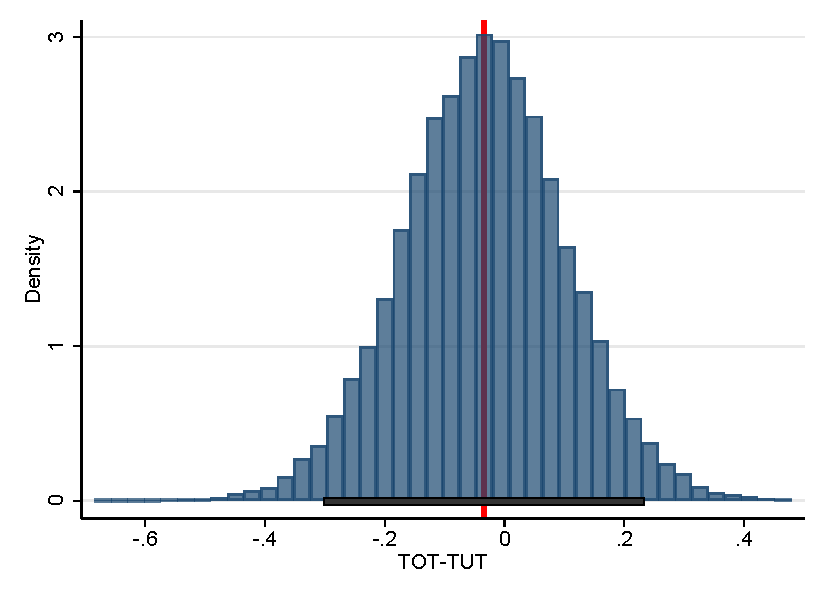
\includegraphics[width=\textwidth]{Figuras/tot_tut_btsp3.pdf}
    \end{subfigure}
  
    \end{center}
     \scriptsize  Given that all of the arms are effectively randomly sampled form the same pool, we can also estimate the ToT and TuT with the pooled regression: $Y_i = \beta_0\mathds{1}(Z_i=0)+\beta_1\mathds{1}(Z_i=1)+\beta_2\mathds{1}(Z_i=2)+ \epsilon_i$, and then this test statistic just becomes the F-test on $\frac{\widehat{\beta_2}-\widehat{\beta_0}}{p}$ for the ToT, $\frac{\widehat{\beta_1}-\widehat{\beta_2}}{1-p}$ for the TuT, and an F-test on the difference between these two quantities to test whether the gains are different between compliers and non-compliers. Recognizing the stochastic nature of the compliance rate, we also bootstrap this quantity before running the previous regression. The red line shows the point estimate for the difference between ToT-TuT, and the gray bar in the x-axis shows a 95\% confidence interval for this difference. Panel (a) shows the difference between the ToT and TuT without any controls, while panel (b) and (c) adds admin controls and admin + survey controls respectively.
          %\footnotesize{ \textit{Do file: }  \texttt{tot\_tut.do}}
\end{figure}


\begin{figure}[H]
     \caption{ToT-TuT CDF}
     \label{tot_tut_ecdf}
    \begin{center}
    \begin{subfigure}{0.6\textwidth}
        \centering
        \includegraphics[width=\textwidth]{Figuras/cdf_tot_tut.pdf}
    \end{subfigure}
    \end{center}
    \scriptsize
       Equipped with estimates for the ToT and TuT for each individual $i$ from an Instrumental Random Forest we compute the ECDF for this quantities. The solid line is the ECDF for the ToT, the dashed line is the ECDF for the TuT, and the dotted line plots the difference between the ToT and the TuT - the blue dashed line in the x-axis shows the points where this difference is significant. The bold black interval at the bottom of the graph is the mean for the ToT distribution (0.07), while the gray interval shows the mean for the TuT distribution (0.10).
       
          %\footnotesize{ \textit{Do file: }  \texttt{tot\_tut\_insforest.do}}
\end{figure}

\begin{figure}[H]
     \caption{Exclusion restriction}
     \label{exclusion_restriction}
    \begin{center}
    \begin{subfigure}{0.6\textwidth}
        \centering
        \includegraphics[width=\textwidth]{Figuras/exclusion_restriction.pdf}
    \end{subfigure}
    \end{center}
    \scriptsize This figure serves as a test for the exclusion restriction in the point identification for the ToT and the TuT. It shows the effect on the effective cost/loan ratio for the forced-fee arm and the choice arm, together with the decomposition of the choosers and non-choosers. Note that a) being forced into the treatment (Forced fee) has the same effect as choosing it (Choosers), and b) not choosing the treatment (Non chooser) has no effect with respect to the control.
    
          %\footnotesize{ \textit{Do file: }  \texttt{exclusion\_restriction.do}}
\end{figure}

%---------------------------------------------------------------------------------------------------------------------------------------------------------------------------------------------------------------------------------

\newpage 
\newpage
\subsection{Causal Random Forest and HTE}

\vspace{.3in}



\begin{figure}[H]
     \caption{Heterogeneous Treatment Effects}
    \label{heterogeneous_effects}
    \begin{center}
    \begin{subfigure}{.45\textwidth}
      \caption{Financial cost (in MXN)}
        \centering
        \includegraphics[width=\textwidth]{Figuras/he_dist_fc_admin_pro_2.pdf}
    \end{subfigure}
     \begin{subfigure}{0.45\textwidth}
    \caption{Effective APR}
       \centering
      \includegraphics[width=\textwidth]{Figuras/he_dist_apr_pro_2.pdf}
    \end{subfigure}
     \begin{subfigure}{0.45\textwidth}
    \caption{Default}
       \centering
      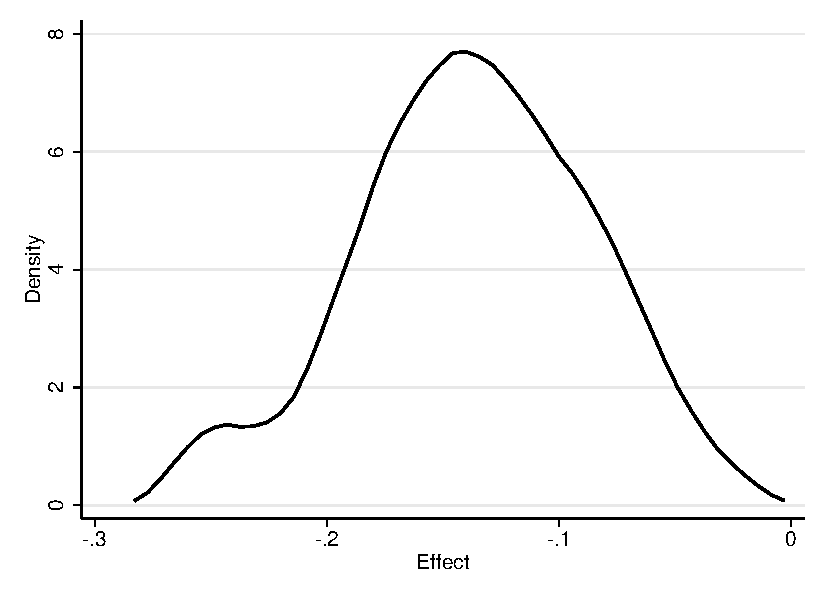
\includegraphics[width=\textwidth]{Figuras/he_dist_def_c_pro_2.pdf}
    \end{subfigure}  
     \begin{subfigure}{0.45\textwidth}
    \caption{Recovery}
       \centering
      \includegraphics[width=\textwidth]{Figuras/he_dist_des_c_pro_2.pdf}
    \end{subfigure}      
    \end{center}
         \scriptsize
     plots the distribution of the heterogeneous treatment effects on financial cost, estimated using \cite{atheygrf}.
  %\footnotesize{ } \textit{Do file: }  \texttt{analyze\_grf\_single\_arm.do}
\end{figure}

\begin{figure}[H]
        \caption{Honest causal tree for the Forced-commitment contract heterogeneous treatment effects}
    \label{casual_tree}
    \begin{center}
        \centering
        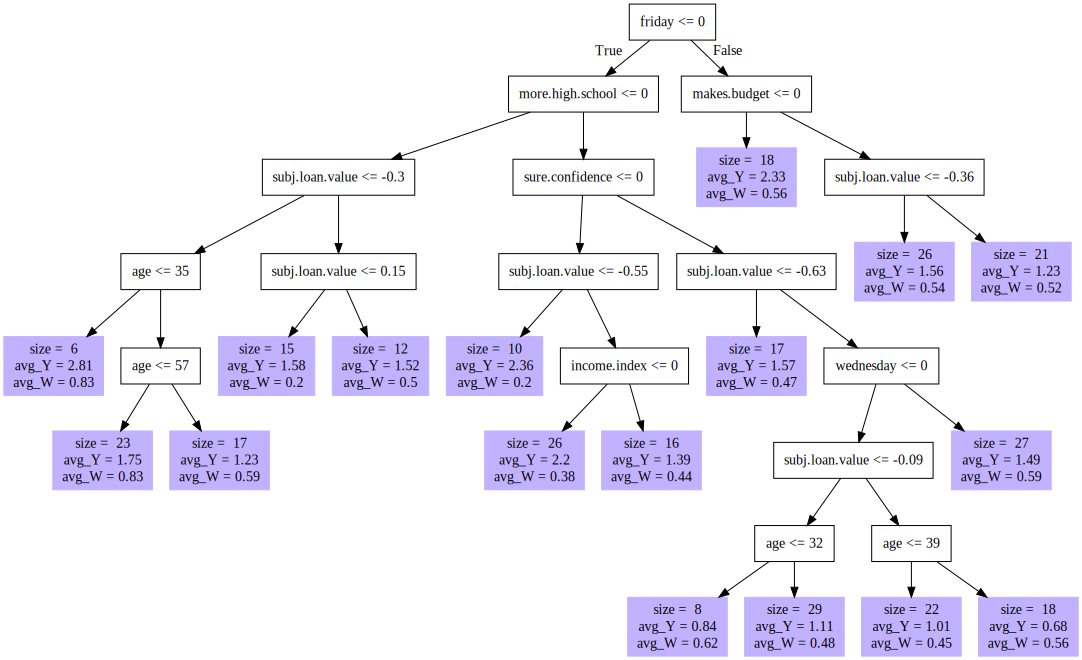
\includegraphics[width=\textwidth]{Figuras/crf_pro_2_apr.pdf}
    \end{center}
    \footnotesize 
    This is one(it is chosen such that it minimizes the pruned cost, that is it is the tree with the smallest root-node impurity) of the honest causal trees in the random forest we use for the estimation of the heterogeneous treatment effect of the fee-forcing contract. It is meant only as an example of how these trees look like. The forest was such that there are as many estimated treatment effects as there are clients.
     %\footnotesize{ \textit{RScript: }  \texttt{grf.R}
\end{figure}

We use \cite{atheygrf} \texttt{causal\_forest} of the \texttt{grf} library in $R$. The parameters used were:
\scriptsize{\textit{causal\_forest(
  X, 
  Y, 
  W, 
  Y.hat = NULL, 
  W.hat = NULL, 
  num.trees = 2000, 
  sample.weights = NULL, 
  clusters = NULL, 
  equalize.cluster.weights = FALSE, 
  sample.fraction = 0.5, 
  mtry = min(ceiling(sqrt(ncol(X)) + 20),ncol(X)), 
  min.node.size = 5, 
  honesty = TRUE, 
  honesty.fraction = 0.5, 
  honesty.prune.leaves = TRUE, 
  alpha = 0.05, 
  imbalance.penalty = 0, 
  stabilize.splits = TRUE, 
  ci.group.size = 2, 
  tune.parameters = "none", 
  tune.num.trees = 200, 
  tune.num.reps = 50, 
  tune.num.draws = 1000, 
  compute.oob.predictions = TRUE, 
  orthog.boosting = FALSE, 
  num.threads = NULL)}}


\begin{figure}[H]
        \caption{Single causal tree for the Forced-commitment contract heterogeneous treatment effects}
    \label{casual_tree}
    \begin{center}
        \centering
        \includegraphics[width=\textwidth]{Figuras/ct_pro_2_apr.pdf}
    \end{center}
    \footnotesize 
   
     %\footnotesize{ \textit{RScript: }  \texttt{grf.R}
\end{figure}





\begin{figure}[H]
    \caption{Choice of contracts and treatment effects}
    \label{choose_wrong}
    \begin{center}
        \begin{subfigure}{0.45\textwidth}
        \caption{Mistakes in choice arm}
        \centering
        \includegraphics[width=\textwidth]{Figuras/line_cw_apr_te_cf.pdf}
        
    \end{subfigure}
        \begin{subfigure}{0.45\textwidth}
        \caption{Financial value of mistake}
        \centering
        \includegraphics[width=\textwidth]{Figuras/money_cw_apr_te_cf.pdf}

    \bigskip
        
    \end{subfigure}
        \begin{subfigure}{0.45\textwidth}
        \caption{\% better when forced to forced commitment}
        \centering
        \includegraphics[width=\textwidth]{Figuras/line_better_forceall_apr_te_cf.pdf}
        
    \end{subfigure}
    %     \begin{subfigure}{0.45\textwidth}
    %     \caption{\footnotesize{Effect of CATE benefit vs predicted take-up}}
    %     \centering
    %     \includegraphics[width=\textwidth]{Figuras/benefit_choice.pdf}% takeuppr_def.pdf 
    % \end{subfigure}
    
    \end{center}
        \scriptsize
        In Panel (a) we estimate what the treatment effect of the commitment contract \textit{would have been} for all subjects in the choice arm if they had been forced into the fee-commitment contract. To do this we proceed in two steps. First, we estimate treatment effects in the forcing arm by comparing the Forced Commitment arm against the status quo arm. We let these effects be heterogeneous as a function of our $x$'s using \cite{atheygrf}'s methodology of causal forests. Second, we extrapolate these treatment effects based on the choice arm using the same $x$'s. Once we have personalized counterfactual treatment effects in the choice arm we calculate what fraction of subjects in the choice arm incurred in financial costs that are  $> z$\% than if they had chosen the opposite contract of what they actually chose, were $z$\% is defined as a fraction of the loan. $z$\% is a level of tolerance we can vary and we plot it in the X-axis. The left Y-axis measures the fraction of subjects that would have been better by a margin of $z$\% if they changed their choice, and the right Y-axis measures the amount of money ``left on the table''. We use bootstrap to tighten the confidence intervals (CIs). \cite{atheygrf}'s heterogeneous treatment effect using GRF is asymptotically normal. We compute the HTE ($\mu$) together with standard errors ($\sigma$) . For every pledge, we draw a random effect from a normal distribution with parameters ($\mu$,$\sigma^2$), and compute via bootstrap the percentage that choose wrong, along normal-approximation CIs (results are robust if we use instead percentile CIs or bias-corrected CIs) . This allows us to estimate a distribution for the upper and lower bound CIs, which we then use to obtain a 95\% CI. Panel (b) is analogous to Panel (a) except that it does the exercise separately for clients we classified as overconfident ($OC_i:=\mathbbm{1}(P^s_i-\widehat{P_i(X_i)}>0))$ and those we classified as not overconfident. Panel (c) simulates what percentage would be better by at least $z$ if we forced everybody of those in the Commitment Choice arm into the fee-commitment contract.
        % Panel (d) asks whether it is the case that people with larger causal benefits from the Forced Commitment contract would be more likely to select that contract. To do this we proceed in two steps as well. First we estimate a flexible model of take-up of the fee commitment contract \textit{in the choice arm} using random forests, and from this model obtain a probability $P(x_i)$ of choosing the Forced Commitment contract for a client with characteristics $x_i$. We extrapolate this model to clients in the Forced Commitment arm to estimate what would they have chosen if we had given them choice. 
        % Figure (d) plots $\widehat{P(x_i)}$ in the X-axis using a binscatter that splits the X-axis in 100 percentile bins. The Y-axis plots the heterogeneous treatment effects of the fee forcing contract on the probability of losing the pawns (more negative means then more likely to recover it), averaged for the respective x-axis bin. Positive assortative selection would mean a negative relationship: those who benefit more by treatment and lose the pawn less are \emph{less} likely to choose it.  Using all bins we estimate a slope of zero in the relationship. Using the 80 right most points, we estimate a \textit{positive} relationship.
        %\textit{Do file: }  \texttt{choose\_wrong\_quant\_wrong.do, choose\_wrong\_quant\_wrong\_decomposition.do}
\end{figure}






\subsection{Take up}


\begin{table}[H]
    \caption{Predicting Take-up: Goodness-of-Fit}
    \label{Table_compliance}
    %\begin{subtable}{1\textwidth}
    % \centering
    %    \caption{Take up}
    %    \scriptsize{% Table generated by Excel2LaTeX from sheet 'oos_pago_frec_vol'
\begin{tabular}{lcccc}
\toprule
      & \multicolumn{4}{c}{Choice} \\
\midrule
\midrule
GOF measures & Logit & SW-Logit & RF    & Boosting \\
\midrule
\midrule
AUC (out of sample) & 0.77  & 0.76  & 0.8   & 0.77 \\
      & (0.04) & (0.04) & (0.04) & (0.04) \\
AUC (in sample) & 0.76  & 0.75  & 0.87  & 0.84 \\
      & (0.02) & (0.02) & (0.01) & (0.01) \\
Accuracy & 0.77  & 0.78  & 0.75  & 0.78 \\
\bottomrule
\bottomrule
\end{tabular}%
}
    %\end{subtable}%
    
    %\bigskip
     \begin{subtable}{1\textwidth}
      \centering
        \caption{Take up: Choice-fee Arm}
        \scriptsize{% Table generated by Excel2LaTeX from sheet 'oos_pago_frec_vol_fee'
\begin{tabular}{lcccc}
\toprule
      & \multicolumn{4}{c}{Frequent voluntary payment - FEE} \\
\midrule
\midrule
OOS measures & Logit & SW-Logit & RF    & Boosting \\
\midrule
\midrule
MAE   & 0.21  & 0.21  & 0.23  & 0.17 \\
MSE   & 0.1   & 0.1   & 0.1   & 0.09 \\
AUC (out of sample) & 0.76  & 0.78  & 0.84  & 0.85 \\
      & (0.06) & (0.06) & (0.06) & (0.05) \\
AUC (in sample) & 0.84  & 0.82  & 0.92  & 0.99 \\
      & (0.02) & (0.02) & (0.01) & (0.01) \\
Accuracy & 0.82  & 0.84  & 0.86  & 0.88 \\
Correlation (0-1) & 0.13  & 0.26  & 0.37  & 0.31 \\
Correlation (predicted val) & 0.33  & 0.38  & 0.37  & 0.43 \\
R-squared  & 0.08  & 0.13  & 0.11  & 0.19 \\
Expected value of predictions & 0.17  & 0.17  & 0.16  & 0.12 \\
\bottomrule
\bottomrule
\end{tabular}%
}
    \end{subtable}
    
      \bigskip
    \begin{subtable}{1\textwidth}
      \centering
        \caption{Take up: Choice-promise Arm}
        \scriptsize{% Table generated by Excel2LaTeX from sheet 'oos_pago_frec_vol_promise'
\begin{tabular}{lcccc}
\toprule
      & \multicolumn{4}{c}{Choice-Promise Arm} \\
\midrule
\midrule
GOF measures & Logit & SW-Logit & RF    & Boosting \\
\midrule
\midrule
AUC (out of sample) & 0.63  & 0.63  & 0.7   & 0.72 \\
      & (0.06) & (0.06) & (0.06) & (0.06) \\
AUC (in sample) & 0.83  & 0.82  & 0.9   & 0.97 \\
      & (0.02) & (0.02) & (0.01) & (0.01) \\
Accuracy & 0.62  & 0.67  & 0.65  & 0.7 \\
\bottomrule
\bottomrule
\end{tabular}%
}
    \end{subtable}
            \scriptsize
           \\
           \\
           \\
    
     %\textit{Scripts: } \texttt{pred\_take\_up.do, pfv\_pred.R}
\end{table}




\vspace{.1in}
\begin{figure}[H]
    \caption{Out of sample ROC curve}
    \label{roc_curve}
    \begin{center}
    \begin{subfigure}{0.45\textwidth}
        \caption{Take-up in Fee Arm}
        \centering
        \includegraphics[width=\textwidth]{Figuras/Boost/ROC_curve_outsample_pago_frec_vol_fee.pdf}
    \end{subfigure}
    \begin{subfigure}{0.45\textwidth}
        \caption{Take-up in Promise Arm}
        \centering
        \includegraphics[width=\textwidth]{Figuras/Boost/ROC_curve_outsample_pago_frec_vol_promise.pdf}
    \end{subfigure}
    \end{center}
     \scriptsize 
  %\footnotesize{ \textit{Do file: }  \texttt{pred\_take\_up.do}}
\end{figure}



\begin{figure}[H]
    \caption{Predictors of commitment contract take-up}
    \label{interactions_takeup}
    \begin{center}
    \begin{subfigure}{0.45\textwidth}
        \caption{PLM}
        \centering
        \includegraphics[width=\textwidth]{Figuras/determinants_takeup_reg.pdf}
    \end{subfigure}
    \begin{subfigure}{0.45\textwidth}
        \caption{Logit}
        \centering
        \includegraphics[width=\textwidth]{Figuras/determinants_takeup_logit.pdf}
    \end{subfigure}
    \end{center}
     \scriptsize
      %\footnotesize{ \textit{Do file: }  \texttt{determinants_takeup.do}}
\end{figure}


\scriptsize 
\noindent This figure reports bivariate (and multivariate) regressions of the form $TakeUp = \alpha + \beta \: X_i + \epsilon_i$. The figure reports the $\beta$ coefficients for different $X_i$'s along with 95\% confidence intervals. Panel (a) uses a linear model. Panel (b) specifies a logit model.

\subsection{Selection on gains}


\begin{figure}[H]
    \caption{Determinants of treatment effects and probability of choosing commitment}
    \label{determinants_ps_hte}
    \begin{center}
    \begin{subfigure}{0.475\textwidth}
        \caption{Determinants of HTE}
        \centering
        \includegraphics[width=\textwidth]{Figuras/HE/he_int_vertical_apr_pro_2.pdf}
    \end{subfigure}
    \begin{subfigure}{0.475\textwidth}
        \caption{Determinants of propensity score}
        \centering
        \includegraphics[width=\textwidth]{Figuras/HE/ps_int_vertical_pr_gbc_1.pdf}
    \end{subfigure}
  
    \end{center}
     \scriptsize   This figure estimates bivariate regressions of the estimated client-level (a) heterogeneous treatment effects, (b) propensity score, against the respective covariate from the baseline survey  $\widehat{HTE_i}, \widehat{P_i} = \alpha + \beta \: X_i + \epsilon_i$. The regressors $X_i$ include (e.g if the family asks for money, if they have savings, if they are overconfident using the definition the text, etc. See this Appendix for a transcription of the survey). \\
      %\footnotesize{ \textit{Do file: }  \texttt{analyze\_grf\_single\_arm.do}} \texttt{benefit\_choice.do}}
\end{figure}



%%%%%%%%%%%%%%%%%%%%%%%%%%%%%%%%%%%%%%%%%%%%%%%
%%%%%%%%%%%%%%%%%%%%%%%%%%%%%%%%%%%%%%%%%%%%%%

% APPENDIX B


\section{ Mechanisms }


\subsection{Optimism, Over-Optimism, and the Failure of Self-Commitment}
\label{overconfidence}

\textcolor{red}{Need to decide whether we want to try to plant our feet on Confidence/Overconfidence as the core `why' of the previous result
.}
%\subsubsection{Behavioral: overconfident borrowers demand less (but benefit more)} \label{behavioral}

The leading behavioral explanation in the literature for low demand for commitment is present biased preferences with naivete (e.g. \cite{Rabin2018}, \cite{John}, \cite{Laibson2018})  \cite{Laibson2015} shows that the lost flexibility resulting from a commitment contract can limit take-up especially severely when agents are (partially) naive about their self control problem. In our context if consumers are (partially) naive about their present bias, they would plan to save more (or spend less) than what they actually end up saving, thus making it be harder to recover their pawn. This under-saving will be mitigated in the fee forcing contract since the fee makes them save money to pay part of the loan periodically. \ref{appendix_c} formalizes this in a model. Another behavioral explanation is that clients may underestimate the likelihood and severity of negative income shocks. Both of these explanations predict that clients will be overconfident about their likelihood of pawn recovery. Recall that in the control group the client's subjective probability of recovery is on average 93\%, while actual recovery is just 44\%. A further piece of evidence consistent with underestimating negative income shocks and with present bias with partial naivete is that a large number of people (25\%) in the control group pay a positive amount toward pawn recovery but end up losing their pawn anyway.


So, overconfidence of recovering the pawn is implied by both present bias preferences with naivete and upward bias in their income expectations. But does overconfidence actually predict low demand for commitment empirically? It does. We define as overconfidence as the reported subjective probability of recovery minus the predicted probability based on the client's characteristics, $P^s_i-\widehat{P_i(X_i)}$.\footnote{We predict $\widehat{P_i(X_i)}$ in two steps. In step one we use Lasso with cross validation to tune the regularization parameter to select the most predictive variables $X$. The typical present bias question as in \cite{Ashraf} was eliminated in this step. In the second step we estimate $\widehat{P_i(X_i)}$ using those variables in a logit model. The Lasso selected variables were type of pawn, female, age, has pawned before, has savings, participates in rotating savings, often feels tempted to change plans, would like to have a reminder to pay, and an economic vulnerability index. We are careful not to include these variables as controls in Table  \ref{oc_reg}.} There is a large amount of overconfidence in our context. Figure \ref{oc_hist} plots a histogram of $OC_i$ and shows that the overwhelming majority display overconfidence, and a large fraction overestimate recovery by more than 50 percentage points. Our measure of overconfidence is useful especially when there is limited time for a detailed survey.\footnote{It may be more useful than a simple elicitation of present bias as in \cite{Ashraf}. We find that 15\% of clients are classified as present biased using this measure of preference reversal. This level is similar to the number \cite{Ashraf} find but small to explain no take-up of commitment for 90\% of clients. This measure was not correlated with take up of commitment in our sample.} First it is very prevalent, which makes it promising to explain the overwhelming prevalence of low take up. Second, it is easy to measure. Third, it is predictive of take-up in an intuitive way. Finally, overconfidence in recovery is implied by present bias with (partial) naivete but also by biased expectations of negative income shocks, thus capturing both kinds of bias.\footnote{\textcolor{red}{Another indication of overconfidence is that in our data, of those who renew, 83\% lose the pawn anyway. Our measure of overconfidence has a correlation of \hl{xxx}\% with a dummy for renewing and losing the pawn. }} 

\cite{Sprenger} have argued that it is critical to understand the link between beliefs and demand for commitment, yet the evidence is scarce. Table \ref{oc_reg} does this: it regresses an indicator of take up of the monthly payment contract against an indicator for overconfidence $OC_i:=\mathbbm{1}(P^s_i-\widehat{P_i(X_i)}>0)$ and controls. Controls $Z$ include branch and day of the week dummies, schooling, whether the client does a monthly budget plan, among others. We are careful not to include controls that were used in $\widehat{P_i(X_i)}$. % and a measure of intertemporal preference reversal analogous to that of \cite{Ashraf} as controls.\
In the choice-fee arm, being overconfident decreases the likelihood of demanding commitment by 12 percentage points a result that this is robust to including controls  (columns 1 and 2). While overconfidence predicts lower take up in the Commitment Choice arm, this is not the case in the promise-choice arm (columns 3 and 4).  One interpretation of the results is that the overconfident borrowers think they do not need commitment, and their demand decreases sharply as soon as there is even a small fee, and at the same time they perceive the promise as a low cost option. This provides evidence for \cite{Sprenger}'s conjecture that ``tepid demand for commitment outside controlled experimental settings is consistent with broad unawareness [of biases]''. 

How does overconfidence map to cost outcomes? Theory predicts that the more overconfident (naive) may be at the same time those that benefit more from commitment. Extrapolating individual treatment effects of the Forced Commitment contract vs the status quo one to the choice arm (see below for more detail), and using them as a dependent variable we find that overconfident borrowers benefit \textit{more} from the commitment contract, with {24.8}\% (=\${30}/\${121}) more savings (columns 5 and 6). Thus while we predict the overconfident benefit more from commitment, they demand less of it. 




\subsubsection{Neoclassical Alternatives} \label{neoclasical}

\vspace{.1in}
\noindent \textbf{Risk aversion.} We do not have measures of risk aversion in our short survey, which makes it hard to assess the hypothesis that risk aversion limits take-up of the fee frequent payment contract. One way to proceed is to take the empirical distribution of financing cost ---$F_{fee}(FC)$--- as one the client would have faced had she chosen the the fee-commitment contract. We could then ask what would risk aversion have to be in order to justify the client choosing the fee-commitment contract distribution of costs over the distribution associated with the status quo contract, $F_{sq}(FC)$. Framed as a choice among cost distributions, we can calculate what risk aversion is needed to rationalize the overwhelming choice of the status quo contract over the fee-commitment contract. This exercise of course assumes --as is common in economics-- that clients know the distribution of financial cost, that the distribution is common across consumers (although this can be relaxed), and that this cost distribution is the only difference among contracts. 

Fortunately for us, it turns out that one distribution first-order-stochastically dominates the other, obviating the need to calibrate a specific utility function or use a parametric distribution function in order to rank them in terms of expected utility. We use the fact that if the utility $u(FC)$ is decreasing in $FC$ (i.e. clients dislike paying higher financing cost) and $F_{fee}(FC) \geq F_{sq}(FC)$ for all $FC$, which we actually verify in our data, then $E_{fee}[u(FC)] \geq E_{sq}[u(FC)]$, that is any expected utility maximizing client risk averse consumer should choose the Forced Commitment contract as a result of the distribution of cost payoffs.\footnote{See the Appendix for the proof. Figure \ref{ecdf_fc} in the Appendix shows that indeed $F_{fee}(FC) \geq F_{sq}(FC)$. Table \ref{stochastic_dominance} shows that this holds also for sub-populations of different characteristics.}. Thus, risk aversion cannot explain the low demand for commitment under the assumptions of this exercise.   


\vspace{.1in}
\noindent \textbf{Lost flexibility.} A second explanation for low take up is lost flexibility. That is, the fee-commitment contract may provide too much commitment which is costly because the client may be forced to incur in late payment fees if he experiences a negative income shock.\footnote{Note that income shocks that affect the ability to pay the entire loan are a worry for both the Forced Commitment contract and the status quo one, and should not make one contract more favorable than the other.} While we cannot rule out that income shocks combined with lost flexibility of the contract explain the low demand, we think it is unlikely. First, we showed above that clients report a subjective probability of recovery of 93\% on average, which suggests they are not too worried about income shocks. Second, the fear of incurring fees is quantitatively not enough of a concern when compared to the savings they are experiencing. %Note that fees for late payment are not that high. In an average loan of 2,000 pesos the monthly payment is close to 700 pesos, and a fee of 2\% of that is 14 pesos (less than \$1 dollar). This is about gr{1\%} of monthly per capita income of the first 3 deciles of Mexican {household's} income distribution. %This compares favorably to the gr{\$11.6 + \$62.3)} pesos transportation / transaction cost of one. 

To make this concrete, we calculated what the financing cost of the fee-commitment contract would be if \textit{all} its clients incurred in \textit{all} potential fees (while keeping payment profiles and pawn recovery constant) and added these fictitious fees to financing cost for those in the Forced Commitment arm, thus artificially inflating their cost. We then re-estimated the quantile treatment effects analogous to Figure \ref{fc_pro2}(b) with this inflated financial cost. %\footnote{Of course behavior may not be constant, but we believe this is a reasonable fist approximation. %It could be that having this small fee added to the balance discourages them to pay or makes it harder to pay back the loan. But the contrary may also happen, with the fee making them more determined to pay early. We would need a structural model of client behavior to estimate a full counterfactual. We suspect that such small fees would not generate large changes in behavior in a simple neoclassical model.}). 
Figure \ref{fc_allfee} presents the results. We find that even in this extreme scenario, tilted against the Forced Commitment contract, the estimated effect still implies cost savings from the Forced Commitment contract at the mean, 25$^{th}$, 50$^{th}$, and 75$^{th}$ percentiles.\footnote{Recall that the differences in financing cost already takes into account the fact that clients in the fee forcing contract sink more pre-payments than those in the status quo contract, and that those prepayments are lost if the loan is not fully paid back.}  Although these arguments are not definitive, they suggest that low demand for commitment may be driven by more than the anticipation of lost flexibility implied by a small fee.

\vspace{.1in}
\noindent \textbf{High time discounting.} We mentioned above that clients in the status quo contract tend to wait until the last moment to pay to recover their pawns. Even among those that recover their pawn, only 40\% pay before the 90$^{th}$ day. Table \ref{mechanisms} shows that clients assigned to the fee-commitment contract front load their payments, starting their first payment earlier and finishing paying earlier too. However, clients may dislike front loading payments if their time preference discount rate is high. They may be willing to trade off a higher probability of losing their pawn for more \textit{back} loaded payments.  

What would discount rates have to be in order for back loaded payments to offset the reductions in financial cost effects we observe? %We can calculate this number by looping across a grid of discount rates, incorporating this higher discount rate in the definition of financial cost, and reestimating equation \ref{basic_reg} with this modified financial cost measure as the dependent variable in equation 1, searching for the discount rate that makes $\beta$ equal zero. We did this and obtained 
We calculate that the discount rate that is necessary to compensate for the savings in financial cost (i.e. that makes the estimated $\beta$ in equation \ref{basic_reg} equal to zero when financing cost --using different $r$'s-- is the dependent variable) is a staggering 8,190 percent per year. We find this discount rate implausibly high even for this credit constrained population\footnote{For comparison, \cite{Levin} find that a discount rate of 1,415 per year for subprime borrowers in the US is too high to be believable.}, casting doubt on high discount rates as explanation for low demand for commitment. %\footnote{In the baseline survey we give respondents a hypothetical choice between $100$ pesos tomorrow or $150$ pesos in one month (an implicit yearly interest rate of {12,800\%}) and only 30\% chose the later one.} 


%%%%%%%%%%%%%%%%%%%%%%%%%%%%%%%%%%%%%%%%%%%%%%%%%%%%%%%%%%%%%%%%%%%%%%%%%%%%%%
%%%%%%%%%%%%%%%%%%%%%%%%%%%%%%%%%%%%%%%%%%%%%%%%%%%%%%%%%%%%%%%%

% APPENDIX C

\newpage
\section{ A simple model}
\label{appendix_c}
\vspace{.2in}
\normalsize
\linespread{1.25}

Although the empirical results are striking and stand alone, this section refers to the model of \cite{John} to interpret our empirical results. The model is stylized but incorporates important features of our context. It allows for negative income shocks which we think are prevalent in this population. %The shock generates a cost of committing to monthly payments and could potentially be a reason for low take up. 
It also features clients with present biased time preferences --allowing for partial naivete-- choosing to save to pay for an expense, and with the opportunity to make a commitment to save and pay. These two features parsimoniously explain several facts about the context --like overconfidence in recovering the pawn--, and about the results --e.g. that forcing commitment seems to help. We intend the model only as a very stylized approximation to our context, and we use it only to help us organize the interpretation of the empirical results, not as a literal description of reality. %Third, it allows for a simple way to model commitment afforded by late payment fees. %Nonetheless, the model abstracts from several details of the context. Even with these abstraction it allows us to explain our six main results listed in Section \ref{explanations_recap} below.

We use the model of \cite{John} and refer the reader to that paper for more detail, justification of assumptions and some of the proofs. The model has three periods and linear utility.\footnote{This does not map perfectly to our 3 period contract, but it is enough to generate the results we need. We also assume that the amount of the loan is used up to pay for the emergency. \cite{John_theory} provides a more general treatment.} Period $t=0$ is a planning period where the client is either allocated to the status quo, the fee-forcing contract, or a choice between the two. Period $t=1$ is the saving-for-the-monthly-payment  period, and $t=2$ in the pawn recovery (loan payment) period. In period 1 the client receives her income $y_1=1$, or gets zero with probability $\lambda$. She can consume ($c_1$) or save ($s_1$) part that income. In period 2 the client gets her savings from period 1, and again receives income of either $y_2=1$, or zero with independent probability $\lambda$. In this last period, she decides whether to use income and savings for consumption $c_2$ and/or for paying back the loan of size $p \in(1,2)$ to recover the pawned piece valued at $b>p$. In this simple set up we model the fee-commitment contract as a contract that imposes a fee of size $F$ if the client fails at $t=1$ to save $s_1=p-1$ pesos, which is what is needed to pay the loan back when there are no shocks. In period $t=0$ she evaluates her welfare as $E[c_1+c_2]$, were for simplicity we have set the time discount to one. We also assume the interest rate is one. We introduce present biased preferences by assuming the following utility function $U_t=c_t+\beta \: \sum_{k=t+1}^{2} E[c_k]$, with $\beta<1$ indicating present bias. A naive client perceives she is not so present biased and instead of $\beta$ uses $\hat{\beta} \in (\beta,1]$. 

Note that under these assumptions it is efficient at $t=0$ to recover the loan since $b>p$ and since there is no discounting at $t=0$. Because $b>1$, paying back the loan requires that there is no negative shock in any period and that $s_1>0$. Because $\beta<1$ at $t=1$ the client will not send savings in excess of what is needed to recover the loan: $s_1=p-1$. This parsimonious model implies the following results:

\vspace{.2in}
\noindent \textbf{Result 1: Present biased clients default more.} Under the status-quo contract, absent shock realizations, present biased clients (sophisticated or naive) with $\beta<\beta_{SQ}<1$ will lose their pawn, while clients with no present bias will not.\footnote{$\beta_{SQ}=\frac{p-1}{\lambda(p-1)+(1-\lambda)(b-1)}$. See Proposition 1 in \cite{John}.} 

\vspace{.1in}
\noindent \textbf{Result 2: Forcing present-biased clients into the fee-commitment contract reduces default.} Imposing a fee $F>0$ for late payments weakly decreases default (for present biased clients only). It strictly decreases default if $F>F_{min}(\beta):=(p-1)-\beta[\lambda(p-1)+(1-\lambda)(b-1)]$. The larger the present bias the larger the $F$ required to induce pawn recovery.\footnote{$F_{min}(\beta)$ is derived from the incentive compatibility constraint needed to generate savings at $t=1$ to recover the pawn can be written as $1-(p-1)+\beta[\lambda(p-1)+(1-\lambda)(b-1)] \geq 1-F+\beta(1-\lambda)$.}

\vspace{.1in}
\noindent \textbf{Result 3: Demand for commitment.} Given $F>0$, (a) Neoclassical clients will never demand commitment. (b) Present-biased sophisticated clients will prefer the fee-forcing contract over the status quo contract $\iff$  $\lambda \: F<(1-\lambda)^2(b-p)$ and $F>F_{min}(\beta)$, that is $\iff$  $\beta \in [\beta_{min},\beta_{SQ}]$.\footnote{$\beta_{SQ}$ was determined in Result 1. $\beta_{min}$ is such that $F=F_{min}(\beta_{min})$.} (c) Analogously, naive clients will demand commitment $\iff$ $\hat{\beta} \in [\widehat{\beta_{min}},\beta_{SQ}]$, where $\widehat{\beta_{min}}<\beta_{min}$. So strongly naive clients will on the one hand demand more commitment than sophisticated clients since they believe (incorrectly) that a smaller fee will motivate them to pay. On the other hand they may demand less commitment since they think they can save and pay on their own. Whether they demand more or less than sophisticated clients depends on the empirical distribution of $\beta$ and $\hat{\beta}$. 

\vspace{.1in}
\noindent \textbf{Result 4: Overconfidence.} Only naive clients will be overconfident about the probability of recovery. This will be true whether they have the status quo or the fee-forcing contract. Overconfidence is increasing in $\hat{\beta}$.

\vspace{.1in}
\noindent \textbf{Result 5: Welfare.} (a) Neoclassical consumers' welfare strictly decreases when we force clients into the fee-commitment contract instead of the status quo contract because of the risk of them not being able to pay for the installment, and does not change when we offer a choice between them. (b) The welfare of sophisticated present biased consumers weakly increases when we give them choice, and it strictly increases  $\iff$  $\beta \in [\beta_{min},\beta_{SQ}]$, that is when they would choose the fee-commitment contract themselves. Forcing them into the fee-commitment contract increases welfare $\iff$  $\beta \in [\beta_{min},\beta_{SQ}]$, otherwise it strictly decreases it. So choice is better than forcing for sophisticates. (c) Forcing can be welfare improving for the naive. Indeed if $\hat{\beta}>\beta_{SQ}>\beta$ then forcing the fee-commitment contract increases welfare, and if $\hat{\beta} \in (\widehat{\beta_{min}},\beta_{min})$ then forcing the status quo contract increases welfare.\footnote{This result is different from that in \cite{John}. Her context has individuals choosing the size of the fee. In that context naive clients will \textit{always} chose the wrong fee size and default later, therefore choice is always decreasing for the naive. In our context $F$ is fixed at 2\% of the balance due, and this implies that choice could be welfare improving for some naifs.} We want to highlight that only under certain parameters will forcing installment payments improve welfare, and that welfare will likely decrease for those with no present bias and the sophisticated present biased consumers. 

\vspace{.1in}
\noindent \textbf{Result 6: Welfare and ex-post observed behavior.} If for a naive client $i$ the fee-forcing contract causes higher pawn recovery, then we know the fee $F$ made her IC constraint binding, and therefore that $\hat{\beta}_i>\widehat{\beta}_{min}$. If in addition if it was the case that $\beta_i<\beta_{SQ}$. %\footnote{\hl{Isaac, aqui tengo dos pregutas: (1) si es $\beta$ y no $\hat{\beta}$ verdad?  (2) Para que una persona naive empenie en el status quo tiene que ser que cree que va a recuperar no? Es decir tiene que ser $\hat{\beta}>\beta_{SQ}$ correcto?}} 
then the fee-forcing contract would have increased welfare for the naive. That is, our finding that the fee-forcing contract increases pawn recovery is a sign of higher welfare (although not a sufficient condition).\footnote{It is not sufficient since ex-ante the commitment $F$ may have been too expensive given the income shocks, i.e. if $\lambda \: F>(1-\lambda)^2(b-p)$.}




\subsection{Interpretation}

The model is very parsimonious but powerful and it can potentially explain all our empirical findings qualitatively.\footnote{The model is sufficiently stylized that we think we would not gain much from estimating it. Furthermore we have no data on income shocks which figure prominently in the model. \cite{Ted} and \cite{Aprajit} are two very recent models that combine a field experiment with commitment contracts and estimation of present bias parameters.} First, it can explain why default is high in the status-quo contract, namely that clients are present biased and have no commitment devices. Second, it can explain why clients are overconfident in our data, namely by virtue of naivete about present bias. Under the model naivete is necessary to explain this. Third, it can also explain why the fee forcing contract induces lower default, but not for everyone: namely that it makes the incentive compatibility constraint for payment binding for the present biased, while it was not binding in the status quo contract. Fourth, it can also explain why there is low demand for commitment even if it seems to improve welfare: namely that there is a small share of neoclassical and sophisticated clients, and at the same time naifs have a present biased parameters values in the region in which they think they can save on their own. Fifth, it explains non-zero demand for commitment for a set of clients. Sixth, it can explain why clients exposed to the Forced Commitment contract are more likely to come back namely those naifs whose welfare increased as a result of being forced into the fee-commitment contract.\footnote{Those with $\hat{\beta_i}>\beta_{SQ}>\beta$.}


\subsection{Other potential explanations: recap} \label{explanations_recap}

There may be other interpretations of the empirical findings, but the bar is high. An alternative explanation will need to explain the 6 facts below:

\begin{enumerate}
\itemsep0em 
\item High (although ex-post inefficient) default in status quo contract.
\item Overconfidence about pawn recovery.
\item Forcing commitment increases pawn recovery.
\item Small demand for commitment...
\item ...but positive demand for commitment.
\item Forcing commitment makes clients more likely to come back.
\end{enumerate}


Let us consider alternative explanations in isolation (i.e. just considering one change or feature at a time with respect to a neoclassical model):

\vspace{.1in}
\noindent \textbf{Alternative 1: Strong prevalence of income shocks.} This could explain (4) and (1), but not why forcing helps, (3) and (6), nor why there is overconfidence, (1). It would also not explain why clients come to pawn in the first place and then default, (2), as they would weight in on the high chance of losing the pawn. 

\vspace{.1in}
\noindent \textbf{Alternative 2: High time discounting}. This could not explain (1) nor (5) nor (6). It could qualitatively explain (4), but as we say in section \ref{sec:demand} quantitatively it would require unbelievably high discount rates.


\vspace{.1in}
\noindent \textbf{Alternative 3: Risk aversion.} We already discussed and rejected risk aversion in section \ref{sec:demand}, although using strong assumptions in the process. Risk or ambiguity aversion could still play a role in explaining 4 and should be investigated in future research. However it would hardly explain (1), (2), (5), or (6).

\vspace{.1in}
\noindent \textbf{Alternative 4: Misunderstanding the contracts.}\footnote{This is a potential criticism of \textit{any} paper offering choice, and one that is non-falsifiable if the critic has free reign to propose how the contracts are perceived in the subject's mind.} We were very aware of the importance of clients understanding the contract in order to infer preferences from choice. That is why we made a strong effort for clients to understand the contracts (see subsection \ref{implementation}). Note however that while clients making purely random mistakes could explain why 10\% demand commitment ---i.e. (4) and (5)--- it would not explain the rest of the findings, nor why the Soft Commitment (see below) had more take up that the fee-commitment, or why we can statistically predict take-up with significant accuracy (see Figure \ref{interactions_takeup} and Table \ref{Table_compliance}).


\vspace{.1in}
\noindent \textbf{Alternative 5 (behavioral): Forgetting to pay/salience.} Frequent payments may act as a reminder to save and recover the pawn. This would try to explain (1) by appealing to people forgetting to pay, and (3), (5), and (6) by appealing to frequent payment acting as reminders (i.e. there being demand for reminders). It would not explain (2) or (4) which are critical in the paper. However even for (1) it seems to us a stretch to explain people losing a valuable pawn by forgetting to pay it. Since the Soft Commitment installment contract did not change behavior (as shown below) this explanation would also require us to posit that only fees acts as reminders, not promises.

\vspace{.1in}
\noindent \textbf{Alternative 6 (behavioral): Income shocks overconfidence}. One could also easily introduce in the overconfidence about income shocks in the model of \ref{appendix_c}\footnote{Say with $\widehat{\lambda} <\lambda$. The effect on demand for commitment is uncertain since on the one hand it decreases $\beta_{SQ}$ decreasing demand, but on the other a smaller $F$ is needed to make the IC binding, making commitment less costly.}. This would leave default unchanged in both the status quo and the fee forcing contract thus would not explain (3), %since $F_{min}(\beta,\widehat{\lambda})<F_{min}(\beta,\lambda)$. 
% $\widehat{\lambda} <\lambda$ alone 
It would not explain (5) or (6) either as demand for commitment would be zero without present bias. 


\vspace{.1in}
We do not claim that the model in the Appendix is the only possible explanation of our empirical findings, but it is a parsimonious explanation of all of them.



%%%%%%%%%%%%%%%%%%%%%%%%%%%%%%%%%%%%%%%%%%%%%%%%%%%%%%%%%%%%%%
%%%%%%%%%%%%%%%%%%%%%%%%%%%%%%%%%%%%%%%%%%%%%%%%%%%%%%%%%%

\clearpage
\bibliographystyle{authordate1}
%\bibliographystyle{amsalpha}
%\bibliographystyle{AER}

\bibliography{References}




% \end{document}

\end{document}
